%% Copernicus Publications Manuscript Preparation Template for LaTeX Submissions
%% ---------------------------------
%% This template should be used for copernicus.cls
%% The class file and some style files are bundled in the Copernicus Latex Package, which can be downloaded from the different journal webpages.
%% For further assistance please contact Copernicus Publications at: production@copernicus.org
%% https://publications.copernicus.org/for_authors/manuscript_preparation.html


%% Please use the following documentclass and journal abbreviations for preprints and final revised papers.

%% 2-column papers and preprints
\documentclass[amt, manuscript]{copernicus}



%% Journal abbreviations (please use the same for preprints and final revised papers)


% Advances in Geosciences (adgeo)
% Advances in Radio Science (ars)
% Advances in Science and Research (asr)
% Advances in Statistical Climatology, Meteorology and Oceanography (ascmo)
% Aerosol Research (ar)
% Annales Geophysicae (angeo)
% Archives Animal Breeding (aab)
% Atmospheric Chemistry and Physics (acp)
% Atmospheric Measurement Techniques (amt)
% Biogeosciences (bg)
% Climate of the Past (cp)
% DEUQUA Special Publications (deuquasp)
% Earth Surface Dynamics (esurf)
% Earth System Dynamics (esd)
% Earth System Science Data (essd)
% E&G Quaternary Science Journal (egqsj)
% EGUsphere (egusphere) | This is only for EGUsphere preprints submitted without relation to an EGU journal.
% Earth Observation (eo)
% European Journal of Mineralogy (ejm)
% Geochronology (gchron)
% Geographica Helvetica (gh)
% Geoscience Communication (gc)
% Geoscientific Instrumentation, Methods and Data Systems (gi)
% Geoscientific Model Development (gmd)
% History of Geo- and Space Sciences (hgss)
% Hydrology and Earth System Sciences (hess)
% Journal of Bone and Joint Infection (jbji)
% Journal of Environmentally Compatible Air Transport System (jecats)
% Journal of Micropalaeontology (jm)
% Journal of Sensors and Sensor Systems (jsss)
% Magnetic Resonance (mr)
% Mechanical Sciences (ms)
% Natural Hazards and Earth System Sciences (nhess)
% Nonlinear Processes in Geophysics (npg)
% Ocean Science (os)
% Polarforschung - Journal of the German Society for Polar Research (polf)
% Proceedings of the International Association of Hydrological Sciences (piahs)
% Proceedings of the International Ocean Drilling Programme (piodp)
% Safety of Nuclear Waste Disposal (sand)
% Scientific Drilling (sd)
% SOIL (soil)
% Solid Earth (se)
% State of the Planet (sp)
% The Cryosphere (tc)
% Weather and Climate Dynamics (wcd)
% Web Ecology (we)
% Wind Energy Science (wes)


%% \usepackage commands included in the copernicus.cls:
%\usepackage[german, english]{babel}
%\usepackage{tabularx}
%\usepackage{cancel}
%\usepackage{multirow}
%\usepackage{supertabular}
%\usepackage{algorithmic}
%\usepackage{algorithm}
%\usepackage{amsthm}
%\usepackage{float}
%\usepackage{subfig}
%\usepackage{rotating}
\usepackage{booktabs}
% \usepackage{tabularx}
\usepackage[version=4]{mhchem}         % module for chemical expression
\usepackage{amsmath,amssymb,bm}
\usepackage{longtable}
\usepackage{placeins}

\newcommand{\xco}{$\mathrm{X_{CO2}}$}
\newcommand{\xcooco}{$\mathrm{X_{CO2}^{OCO-2}}$}
\newcommand{\xcotccon}{$\mathrm{X_{CO2}^{TCCON}}$}
\newcommand{\xcobc}{$\mathrm{X_{CO2}^{B11}}$}
\newcommand{\xcoraw}{$\mathrm{X_{CO2}^{raw}}$}
\newcommand{\xcoprior}{$\mathrm{X_{CO2}^{prior}}$}
\newcommand{\xcoatom}{$\mathrm{X_{CO2}^{ATom}}$}
\newcommand{\xcoship}{$\mathrm{X_{CO2}^{Ship}}$}
\newcommand{\xcode}{$\mathrm{X_{CO2}^{DE}}$}


\begin{document}

\title{An Imager-free, Footprint-level Correction of Cloud-induced Biases in OCO-2 $\mathrm{X_{CO2}}$ using Photon Path-length Statistics and Deep Ensembles}


% \Author[affil]{given_name}{surname}

\Author[1,2][Yu-Wen.Chen@colorado.edu]{Yu-Wen}{Chen} %% correspondence author
\Author[1,2]{Ken}{Hirata}
\Author[1,2]{Sebastian}{Schmidt}

\affil[1]{Department of Atmospheric and Oceanic Science, University of Colorado, Boulder, Boulder, CO, USA}
\affil[2]{Laboratory for Atmospheric and Space Physics, University of Colorado, Boulder, Boulder, CO, USA}

%% The [] brackets identify the author with the corresponding affiliation. 1, 2, 3, etc. should be inserted.

%% If an author is deceased, please add \deceased[$Deceased date if applicable$]{$Author number$} (e.g. \deceased[13 November 2015]{2}) at the end of the affiliations. The author number depends on the placement of the author in the author list, e.g. the third author has number 3.


%% If authors contributed equally, please add \equalcontrib{$Author numbers$} (e.g. \equalcontrib{1,3}) at the end of the affiliations. The author number depends on the placement of the author in the author list, e.g. the third author has number 3.




\runningtitle{TEXT}

\runningauthor{TEXT}





\received{}
\pubdiscuss{} %% only important for two-stage journals
\revised{}
\accepted{}
\published{}

%% These dates will be inserted by Copernicus Publications during the typesetting process.


\firstpage{1}

\maketitle



\begin{abstract}
TEXT
\end{abstract}


\copyrightstatement{TEXT} %% This section is optional and can be used for copyright transfers.


\introduction  %% \introduction[modified heading if necessary]
\label{sec:intro}


1.1 Scientific and measurement problem

- Establish the role of OCO-2 XCO2 in flux inversions, regional carbon
  budgets, trend monitoring, and emission studies.
- Explain why sub-ppm systematic errors matter.
- Introduce cloud-side illumination, shadowing, and altered photon paths as
  mechanisms affecting nominally clear soundings near clouds.
- Reframe screening as spatially correlated sampling, not merely reduced
  sample size: persistently cloudy regions lose observations preferentially.

Suggested agency-level sentence:

> Cloud screening is therefore not only a loss of sample size: it
> preferentially removes observations from persistently cloudy regions,
> potentially reinforcing spatial sampling biases in atmospheric CO2
> inversions.

1.2 Previous approaches and unresolved gap

Organize the literature by approach:

1. 3-D radiative-transfer characterization of cloud adjacency;
2. MODIS- or imager-dependent empirical corrections;
3. general retrieval bias correction and machine learning;
4. the operational OCO-2 bias-correction chain.

Define the gap narrowly: no existing approach is shown here to combine
physical interpretation, single-footprint inference without an imager,
probabilistic uncertainty, independent validation, and explicit
plume-preservation tests.

Avoid claiming that the operational B11 correction is not cloud-aware in any
sense. The supported statement is that it does not fully resolve the observed
surface-dependent near-cloud residuals and can over-correct near-cloud land
soundings in this evaluation.

1.3 Questions and contributions

Frame the study around four questions:

1. Do nominally clear OCO-2 spectra contain a measurable signature of nearby
   clouds?
2. Can photon path-length statistics explain the land–ocean difference in
   XCO2 response?
3. Can a per-footprint model reduce independent-reference error without cloud
   distance at inference?
4. Does the correction preserve real CO2 enhancements, and where does it
   fail?

End with five contributions:

- spectrum-derived photon path-length diagnostics;
- a surface-specific probabilistic correction;
- date-blocked, leakage-guarded evaluation;
- independent TCCON, ATom, and shipborne validation;
- smoother, feature-ablation, plume-preservation, and failure-mode tests.

State deployment independence here. Reserve the full three-tier
imager-independence argument for the Discussion.




%\section{HEADING}
%TEXT


%\subsection{HEADING}
%TEXT


%\subsubsection{HEADING}
%TEXT

\section{Data}
\label{sec:data}

\subsubsection*{OCO-2 data}
This research uses OCO-2 version 11 data to analyze and compare the data. We use the v11r and v11.2r level 2 meteorological data (OCO2\_L2\_Met) and \ce{CO2} prior data (OCO2\_L2\_CO2Prior) for the atmospheric pressure, temperature, water vapor, \ce{O2}, and \ce{CO2} profiles \citep{oco2_l2_co2prior_11r, oco2_l2_co2prior_112r, oco2_l2_met_11r, oco2_l2_met_112r}. The version 5.2 ACOS/OCO-2/OCO-3 absorption coefficient (ABSCO) lookup  tables are used to calculate the gas absorption optical depths \citep{oco2_absco_tables_v52}. The level 1B version v11r and version v11.2r data provide detailed geometry information and calibrated spectra \citep{oco2_l1b_science_11r, oco2_l1b_science_112r}. The calibrated \ce{O2}A, \ce{WCO2}, and \ce{SCO2} spectra are used to fit the photon path parameters. The version 11r and 11.2r are used depend on dates before or after April 1st, 2024. Variables from full-physics retrieval results and the operational bias-corrected $\mathrm{X_{CO2}}$, $\mathrm{X_{CO2}^{B11}}$ of the v11.2r and v11.3r (before and after April 1st, 2024) Lite product are used for data anlysis, bias-correction training, and correction comparison \citep{oco2_l2_lite_fp_112r, oco2_l2_lite_fp_113r}. All nadir, glint, and target modes for ocean and land with quality flags of 0 and 1 are used in the analysis. 



\subsubsection*{MODIS products}
Because OCO-2 and MODIS Aqua satellites were both flying along A-train orbit, with only 6 minutes away, MODIS Aqua data are good information about the nearby conditions for OCO-2 footprints. We used MODIS Aqua 1km Geolocation data (MYD03, collection 6.1) and Cloud Mask and Spectral Test Results (MYD35, collection 6.1) as the truth for cloud locations near OCO-2 footprints \citep{myd03_061, myd35_l2_061}. Cloudy and uncertain classes are utilized to calculate the nearest cloud distance for OCO-2 footprints. See details in \ref{sec:method-cld_dist_xco2_anom}. Note that the cloud distance derived from MODIS products contributes to target construction and analysis only, it is not supplied to the correction model. In addition to MODIS cloud products, we also use MODIS yearly land cover type (MCD12C1, collection 6.1) for data anlysis and Aqua RGB imagery for data visualization \citep{friedl2022mcd12c1_v061}.


\subsubsection*{Independent reference observations}
We compared the $\mathrm{X_{CO2}^{B11}}$ and cloud-proximity-corrected $\mathrm{X_{CO2}}$ ($\mathrm{X_{CO2}^{corr}}$) against TCCON GGG2020 data \citep{laughner2024ggg2020} from the stations listed in Table \ref{tab:tccon-stations-used}. In addition to TCCON data, we also used airborne in-situ measurements from the Atmospheric Tomography Mission (ATom) to create pseudo-column $\mathrm{X_{CO2}}$ ($\mathrm{X_{CO2}^{ATom}}$) and shipborne EM27/SUN measurements during the Measuring Ocean REferences 2 (MORE-2) campaign in June 2019 and the research vessel Mirai campaign MR21-01 in 2021 as additional OCO-2 ocean footprints comparison \citep{wofsy2018atom_nav, mckain2021atom_picarro, knapp2020more2_pangaea, hanft2021mr2101_pangaea}. We apply the averaging-kernel and prior harmonization for comparison between $\mathrm{X_{CO2}^{corr}}$ and $\mathrm{X_{CO2}^{TCCON}}$, with details described in Section \ref{sec:method-eval-obs-xco2} and Appendix \ref{app:ak_operation}. The conversion of pseudo-column $\mathrm{X_{CO2}^{ATom}}$ from in-situ \ce{CO2} mixing ratios is discuessed in \ref{sec:method-eval-obs-xco2}.

%%%
%Throughout, $X_{CO2}^{B11}$ denotes the operationally bias-corrected XCO2 of the OCO-2 v11 Lite product (the xco2 variable; O'Dell et al., 2018), and $X_{CO2}^{corr} = X_{CO2}^{B11} - \mu$ denotes our cloud-proximity-corrected product, where $\mu$ is the per-sounding bias predicted by the deep ensemble.







% plume-overpass catalogues

\section{Methods}

\subsection{Cloud-distance calculation and within-orbit anomaly}
\label{sec:method-cld_dist_xco2_anom}

The nearest cloud distance is defined geometrically, independent of any spectral or OCO-2 retrieval quantity. The cloud set $\mathcal{C}$ pools the MYD35 \emph{Cloudy} and \emph{Uncertain} classes (Sect.~\ref{sec:data}). We excludes \emph{Probably clear} and \emph{Confident clear} pixels in the calculation, so distance is measured to the nearest \emph{non-clear} MODIS pixel. To avoid the meridian-convergence and polar distortions of a latitude--longitude metric, each OCO-2 footprint center $(\varphi_i,\lambda_i)$ and each cloud pixel $(\varphi^{c}_m,\lambda^{c}_m)$ is mapped to Earth-Centred, Earth-Fixed (ECEF) Cartesian coordinates $\mathbf{r}$ on the WGS84 ellipsoid, both placed on the reference surface ($h=0$) so that proximity is horizontal and does not use cloud-top height. The nearest-cloud distance is the minimum Euclidean distance in ECEF space,
%
\begin{equation}
  d_i \;=\; \min_{m\in\mathcal{C}}
  \bigl\lVert\, \mathbf{r}_i - \mathbf{r}^{c}_m \,\bigr\rVert_{2},
  \label{eq:cloud-distance}
\end{equation}
%
evaluated with a $k$--$d$ tree over $\mathcal{C}$; the chord metric is monotone
in the great-circle arc, so it returns the same nearest pixel and, over the
sub-$50$~km range of interest, differs from the geodesic distance by less than
the $1$~km MODIS pixel scale. The reported distance is capped at
$d_{\max} = 50\;\mathrm{km}$. Soundings whose local search contains no cloud
pixel are assigned $d_i = d_{\max}$ (\emph{No\;Cloud}), and post-2022 granules
during the Aqua free-drift period are flagged \emph{No\;MODIS} and excluded from the distance statistics rather than given a numerical distance. The example of the derived nearest cloud distance for OCO-2 footprints is shown in Fig.~\ref{fig:OCO-fp-cld_dist}.

\begin{figure}[t]
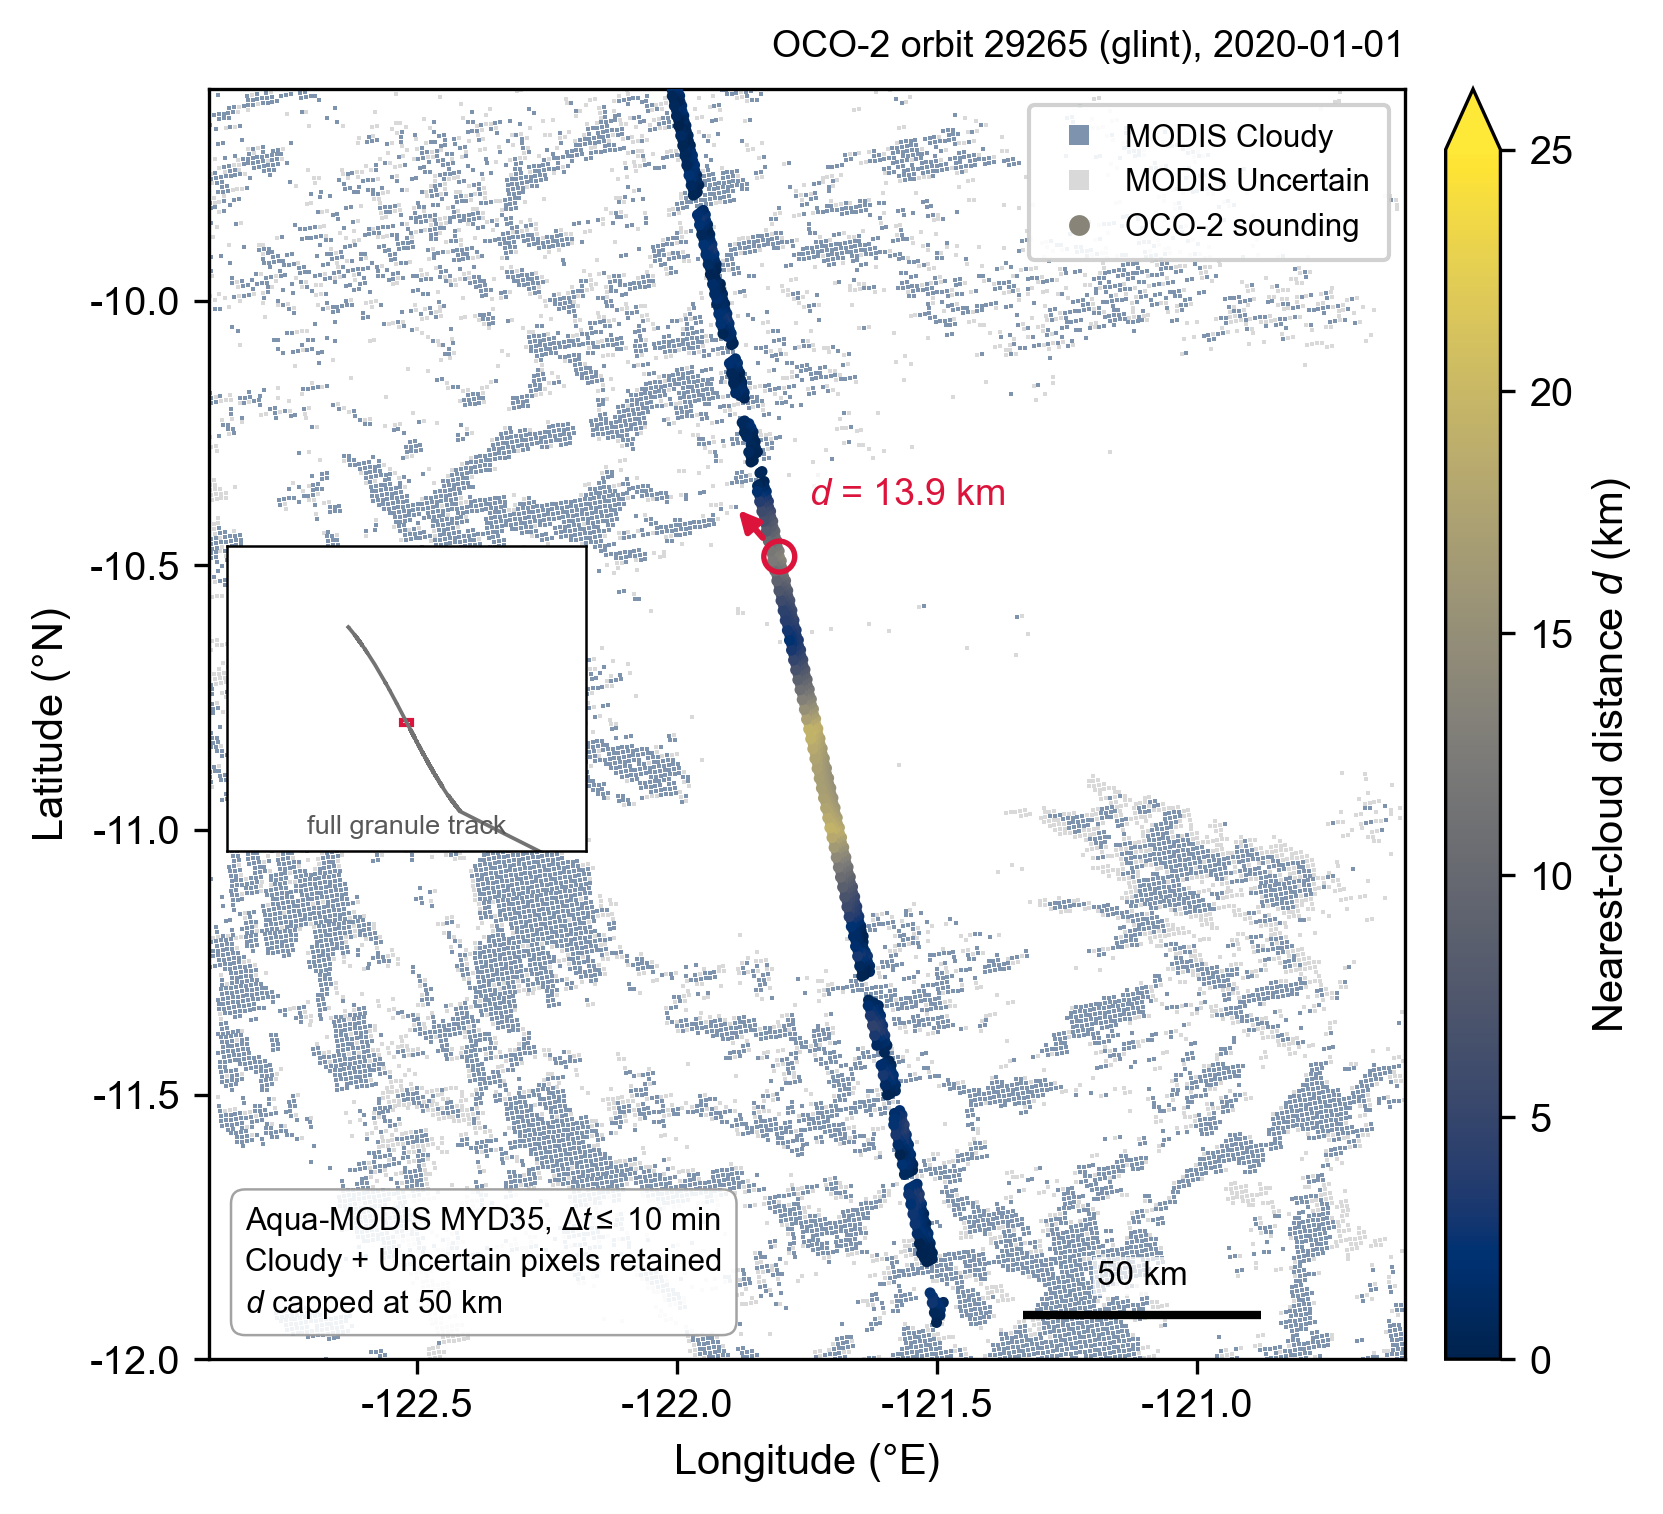
\includegraphics[width=12cm]{figures/fig01_collocation_schematic.png}
\caption{The example of nearest cloud distance result from OCO-2 orbit 29265 on Jan. 1st, 2020.}
\label{fig:OCO-fp-cld_dist}
\end{figure}

\subsubsection{Within-orbit clear-sky anomaly target}

The correction target is an OCO-2-relative $\mathrm{X_{CO2}}$ anomaly that isolates the cloud-proximity signal from the large-scale meridional \ce{CO2} gradient. For sounding $i$, define a local clear-sky reference set from soundings in the same orbit that lie within a latitude half-window $\Delta\varphi$ of $i$ and are far from cloud,
%
\begin{equation}
  \mathcal{R}_i(d_0)
  = \bigl\{\, j :\ |\varphi_j - \varphi_i| \le \Delta\varphi,\
  d_j > d_0,\ \mathrm{X_{CO2,j}}^{\mathrm{B11}}\ \text{valid} \,\bigr\},
  \label{eq:reference-set}
\end{equation}
%
with clear-sky threshold $d_0$ and window $\Delta\varphi = 0.25^{\circ}$. Let
$\mu_i$ and $\sigma_i$ be the mean and standard deviation of the
bias-corrected $\mathrm{X_{CO2,j}}^{\mathrm{B11}}$ over $\mathcal{R}_i(d_0)$. The target is the departure of each sounding from its local clear-sky background,
%
\begin{equation}
  \Delta \mathrm{X_{CO2,i}}^{\mathrm{B11}}
  = \mathrm{X_{CO2,i}}^{\mathrm{B11}} - \mu_i,
  \qquad
  \mu_i = \frac{1}{|\mathcal{R}_i|}
  \sum_{j\in\mathcal{R}_i} \mathrm{X_{CO2,i}}^{\mathrm{B11}},
  \label{eq:anomaly-target}
\end{equation}
%
and is defined only where the reference background is both well populated and
stable,
%
\begin{equation}
  |\mathcal{R}_i| \ge n_{\min} = 5,
  \qquad
  \sigma_i \le \sigma_{\max} = 1.0\ \mathrm{ppm}.
  \label{eq:anomaly-guards}
\end{equation}
%
The population guard $n_{\min}$ suppresses noisy small-sample means, and the
spread guard $\sigma_{\max}$ discards windows where an unresolved
synoptic-scale gradient or residual contamination inflates the reference scatter, or emission sources affect part of footprints in the reference. Soundings failing either test carry no target and are dropped from
training and target-space evaluation.

The clear-sky threshold $d_0$ is the one target parameter. We first use $d_0 = 10$~km to identify the effective cloud-influence distance, and then vary the thresholds by surface: $d_0 = 15$~km over land
(\emph{r15}) and $d_0 = 5$~km over ocean (\emph{r05}), reflecting the different
distance scales at which the land and ocean anomaly--distance curves flatten
(Sect.~\ref{sec:result-cld_dist}). 

We state the principal limitation of this construction at the outset:
Eq.~\eqref{eq:anomaly-target} defines an \emph{OCO-2-relative} anomaly, not an
absolute $\mathrm{X_{CO2}}$ error. The reference mean $\mu_i$ is itself an OCO-2 product and can absorb a genuine within-window atmospheric gradient, so
$\Delta \mathrm{X_{CO2}^{B11}}$ may contain real \ce{CO2} structure in addition to the cloud-induced bias. The stability guard $\sigma_{\max}$ bounds, but does not eliminate, this contamination. Independent validation against TCCON, aircraft, and shipborne references (Sect.~4.5, 4.7) is therefore essential, because it does not rely on the OCO-2-relative target.



\subsection{Spectrum-internal Features from Photon-Path Distribution Function}
\label{sec:methods_photon_path}

%\subsubsection{HEADING}

We derived spectral features based on the photon path distribution function (PPDF) assumptions that summarize the distribution of atmospheric
photon paths represented in each OCO-2 absorption band. The derivation follows
the radiative-transfer equivalence theorem
\citep{irvine1964,partain2000,stephens2000}. 


For a fixed illumination and viewing geometry with solar zenith angle (SZA) and viewing zenith angle (VZA), let $P_0(l)$ denote the ensemble of photon trajectories $l$ from the top of the atmosphere (TOA) reaching the detector in a conservative reference atmosphere with the same surface boundary and continuum scattering properties. The photon trajectories $l$ are mainly determined by multiple-scattering within the atmosphere by air molecules, clouds, and aerosols. Across each narrow OCO-2 band, we assume that these scattering properties vary slowly relative to molecular line absorption, so $P_0(l)$ is the same within each narrow band.  Wavelengths then changes the contribution $w_\lambda$ of a trajectory primarily through its Beer--Lambert survival probability,
%
\begin{equation}
  w_\lambda(l)
  = \exp[-\tau_\lambda(l)],
  \qquad
  \tau_\lambda(l)
  = \int_{l} \alpha_\lambda(s)\,\mathrm{d}s,
  \label{eq:main_path_weight}
\end{equation}
%
where $\alpha_\lambda$ is the local molecular absorption coefficient, and $\tau_\lambda$ is the total optical depth of each photon trajectory $l$.  The
normalized radiance is therefore the conservative-ensemble mean
%
\begin{equation}
  \mathcal T_\lambda
  = \int P_0(l)
      \exp[-\tau_\lambda(l)]\,\mathrm{d}l.
  \label{eq:main_equivalence}
\end{equation}
%
This construction separates the multiple-scattering calculation from molecular
absorption and remains applicable to three-dimensional cloud fields because the
cloud geometry is encoded in $P_0(l)$ \citep{stephens2000}.
%
%
%
For the direct geometrical slant path $L$, we define the modeled molecular slant optical depth $\mathrm{\overline{SOD}}_\lambda$ along $L$,
%
\begin{equation}
  \mathrm{\overline{SOD}}_\lambda
  = \int_0^{L} \tau_\lambda(s)\,\mathrm{d}s,
  \label{eq:main_SOD}
\end{equation}
%

To obtain a tractable scalar representation, we define the relative path length $l'$ for non-absorbing wavelength or an effective absorber-path enhancement relative to the direct geometrical slant as 

\begin{equation}
  l'
  = l/L,
  \label{eq:main_relative_path_length}
\end{equation}

Thus, we can approximate the absorber amount along each trajectory as
\begin{equation}
  A_\lambda(l')
  \simeq \mathrm{\overline{SOD}}_\lambda l',
  \label{eq:main_scalar_path}
\end{equation}

The conservative ensemble induces a normalized distribution $p_0(l')$, so Eq.~\eqref{eq:main_equivalence} reduces to

\begin{equation}
  \mathcal T(\mathrm{\overline{SOD}}_\lambda)
  = \int_0^\infty p_0(l')
      \exp(-\mathrm{\overline{SOD}}_\lambda l')\,\mathrm{d}l'.
  \label{eq:main_laplace}
\end{equation}

Thus, the resolved absorption spectrum samples the Laplace transform of one
wavelength-independent conservative path distribution within each band.  This
does not imply that weak and strong channels detect identical photon
populations: absorption reweights the detected paths as
$p_{\mathrm{det}}(l'\mid\mathrm{SOD})\propto
p_0(l')\exp(-\mathrm{SOD}\cdot l')$, preferentially suppressing long paths at large
$\mathrm{SOD}$.

We normalized the measured radiance as
\begin{equation}
  T_\lambda
  = \frac{\pi I_\lambda}{F_{0,\lambda}^{ILS}\mu_0}
  = \gamma\,\mathcal T(\tau_\lambda),
  \label{eq:main_transmittance}
\end{equation}
where $F_{0,\lambda}^{ILS}$ is the Earth-Sun distance corrected, Doppler stretch corrected, and
ILS-convolved top-of-atmosphere solar irradiance, $\mu_0$ is the
cosine of the SZA, and $\gamma$ is an effective continuum
reflectance.  In practice, $\gamma$ can include surface bidirectional
reflectance, polarization, and surface--atmosphere coupling and is not
interpreted as an exact Lambertian albedo.

Let $C_n$ denote the ordinary cumulants of $p_0(l')$.  Expanding the log
Laplace transform about zero absorption gives
\begin{equation}
  \ln T(\mathrm{\overline{SOD}})
  = \ln\gamma
    + \sum_{n=1}^{\infty}
      \frac{(-1)^n C_n}{n!}\tau^n.
  \label{eq:main_cumulant}
\end{equation}
For each sounding and band, we fitted the truncated form
\begin{equation}
  \ln T(\mathrm{\overline{SOD}})
  \simeq b
    + \sum_{n=1}^{N}
      \frac{(-1)^n k_n}{n}\tau^n,
  \qquad
  k_n=\frac{C_n}{(n-1)!},
  \label{eq:main_fit}
\end{equation}
where $b$ is the fitted continuum intercept.  Under the equivalence-theorem and
scalar-path assumptions, $k_1=\mathrm{E}_{p_0}[l']$ is the mean absorber-path
enhancement and $k_2=\mathrm{var}_{p_0}(l')$ is its variance; coefficients
$k_{n\geq3}$ are scaled higher cumulants.

The model is linear in $(b,k_1,\ldots,k_N)$.  We solved it by singular-value
least squares and used bounded-variable least squares only when the
unconstrained solution violated $k_1,k_2\geq0$.  We excluded the two edge
channels and channels with $T_\lambda>1$.  The truncation orders were 7, 3, and
7 for the O$_2$A, WCO$_2$, and SCO$_2$ bands, respectively; the lower
WCO$_2$ order reflects its smaller optical-depth range and the resulting
poor identifiability of high-order terms. 

We interpret these quantities as \emph{band-effective absorber-path cumulants}.
The scalar approximation in Eq.~\eqref{eq:main_scalar_path} can fail when
pressure- and temperature-dependent line absorption weights atmospheric layers
differently, or when surface, aerosol, or polarization properties vary within a
band.  A layer-resolved formulation and the distinction from a gamma path model
are given in Appendix~\ref{app:spectral_fit_derivation}.










% For a single photon with wavelength $\lambda$ traveling from the top of the atmosphere (TOA) to the satellite sensor along the path $L$, we can express its transmittance $T_\lambda(L)$ as

% \begin{equation}
%     T_\lambda(L)
%     =
%     \exp\left\{-\int_0^L\sum_i \left[\sigma_{i,\lambda}(l)n_i(l)\right]dl\right\}
%     =
%     \exp\left\{-\int_0^L\sum_i \left[\alpha_{i,\lambda}(l)\right]dl\right\}
%     =
%     \exp\left\{-\int_0^L\alpha_{t,\lambda}(l)dl\right\},
% \label{eq:single_photon_transmittance}
% \end{equation}

% where $l$ is the partial path along the total path $L$, $\sigma_{i,\lambda}(l)$ is the extinction coefficient at wavelength $\lambda$ on the path $l$ for gas $i$, $n_i(l)$ is the number concentration of the path $l$ for gas $i$. $\alpha_{i,\lambda}$ is the extinction at $\lambda$ for gas $i$, while $\alpha_{t,\lambda}$ is the total extinction considering all gases.


% For multiple photons, we can calculate an average transmittance $\overline{T_\lambda(\alpha_{t,p}, L_p)}$ as 



% \begin{equation}
% \begin{split}
%     \overline{T_\lambda(\alpha_{t,p}, L_p)}
%     &=
%     \frac{1}{N}\sum_{p=1}^{N}
%     \exp\left\{-\int_0^{L_p}\alpha_{t,p}(l)dl\right\} \\
%     &\approx
%     \frac{1}{N}\sum_{p=1}^{N}
%     \exp\left\{-\int_0^{L_p}\overline{\alpha_t}dl\right\}
%     &=
%     \frac{1}{N}\sum_{p=1}^{N}
%     \exp\left\{\overline{\alpha_t}L_p\right\}
% \end{split}
% \label{eq:multi_photon_transmittance}
% \end{equation}


% where $\alpha_{t,p}(l)$ is the total extinction of the photon $p$ at the partial path $l$, and $L_p$ is the total path length of the photon $p$, $N$ is the total photon number. $\overline{\alpha_t}$ is the vertical mean total extinction, which is independent on photons. \\


% Equation \ref{eq:multi_photon_transmittance} can be expressed in the photon path distribution function $p(L)$


% \begin{equation}
% \begin{split}
%     \overline{T_\lambda(\alpha_{t,p}, L_p)}
%     &=
%     \int_0^{L\to \infty} p(L)
%     \exp\left\{-\overline{\alpha_t}L\right\}dL,
% \end{split}
% \label{eq:multi_photon_transmittance_2}
% \end{equation}

% Now we can define the relative photon path length $L'=L/L_{geo}$, where $L_{geo}$ is the reference geometric photon path length, or the vertical distance from TOA to the surface multiply by the geometric two-way airmass $m$,

% \begin{equation}
% m
% =
% \frac{1}{\cos\theta} + \frac{1}{\cos\phi} ,
% \label{eq:airmass_sod}
% \end{equation}

% where $\theta$ and $\phi$ are the solar and viewing zenith angles.

% \begin{equation}
% L_{geo}
% =
% m\,L_{\mathrm{TOA-surface}} ,
% \label{eq:airmass_photon_path_geo}
% \end{equation}


% \begin{equation}
% \begin{split}
%     \overline{T_\lambda(\alpha_{t,p}, L_p)}
%     &=
%     \int_0^\infty p(L)
%     \exp\left\{-\overline{\alpha_t}L\right\}dL,
% \end{split}
% \label{eq:multi_photon_transmittance_2}
% \end{equation}


% \begin{equation}
% \overline{\mathrm{SOD}}_c(\lambda)
% =
% \bar{\alpha}(\lambda)\bar{L},
% \label{eq:slant_optical_depth}
% \end{equation}


% For each footprint and spectral band, we use an
% instrument lineshape-convolved effective slant optical depth,
% $\overline{\mathrm{SOD}}_c$, as the spectral coordinate. The high-resolution
% vertical optical depth ($\tau_v(\lambda)\}$) is first multiplied by the geometric two-way airmass,






% The slant optical depth is then computed in transmission space,
% \begin{equation}
% \overline{\mathrm{SOD}}_j
% =
% -\ln
% \left[
% \frac{
% \sum_q R_j(\lambda_q)
% \exp\{-m\tau_v(\lambda_q)\}
% }{
% \sum_q R_j(\lambda_q)
% }
% \right],
% \label{eq:ils_sod}
% \end{equation}
% where $j$ indexes the discrete wavelength samples in an OCO-2 band and
% $q$ indexes the high-resolution wavelength grid used for the ILS convolution. $R_j(\lambda)$ is the instrument lineshape (ILS) for pixel or discrete wavelength $j$ and $\tau_v(\lambda_q)$ is the high-resolution vertical optical depth, including molecular absorption and Rayleigh extinction.




% The measured spectral transmittance used in the fit is
% \begin{equation}
% T(\lambda)
% =
% \frac{\pi I(\lambda)}{\mathcal{F}_{0}^{ILS}(\lambda)\cos\theta},
% \label{eq:measured_transmittance}
% \end{equation}

% where $I(\lambda)$ is the calibrated OCO-2 radiance and $\mathcal{F}_{0}^{ILS}(\lambda)$ is the Earth-Sun distance corrected, Doppler stretch corrected, and
% ILS-convolved solar normalization used in the spectral fit. See details in \ref{eq:solar_distance_doppler}, \ref{eq:solar_ils_convolution}, \ref{eq:effective_solar_normalization}.











% \begin{equation}
% T(\overline{\mathrm{SOD}}_c)
% =
% \gamma
% \int_0^\infty
% p(l')
% \exp(-\overline{\mathrm{SOD}}_c \; l')
% \,\mathrm{d}l' ,
% \label{eq:transmittance_laplace}
% \end{equation}

% \begin{equation}
% \ln T(\overline{\mathrm{SOD}}_c)
% =
% \ln\gamma
% +
% \sum_{n=1}^{N}
% (-1)^n
% \frac{k_n}{n}
% \overline{\mathrm{SOD}}_c^n .
% \label{eq:cumulant_fit}
% \end{equation}


% \begin{equation}
% k_1 = \langle l' \rangle,
% \qquad
% k_2 = \operatorname{var}(l'),
% \qquad
% \kappa = \frac{k_1^2}{k_2}.
% \label{eq:coefficient_interpretation}
% \end{equation}


\subsection{Predictors and probabilistic model}
\label{sec:methods-models}


After deriving the \emph{OCO-2-relative} anomaly ($\Delta \mathrm{X_{CO2}^{B11}}$) in Sect.\ref{sec:method-cld_dist_xco2_anom} and the photon path-length features in Sect.\ref{sec:methods_photon_path}, we build deep-ensemble multilayer perceptron (\emph{DE-MLP}) models to predict and correct $\Delta \mathrm{X_{CO2}^{B11}}$. Separate models are trained for land and ocean footprints. We also compare the model performance with ridge linear regression (\emph{Ridge}) and gradient-boosted decision trees (\emph{XGBoost}) models.

We use $\Delta \mathrm{X_{CO2}^{B11}}$ as the truth for training, and features from photon path-length fitting (Sect.\ref{sec:methods_photon_path}), full-physics retrieved variables in the lite files, EOFs of temperature, water vapor, and \ce{CO2} profiles, geometry and L1B diagnostics, contamination indicators, and a one-hot-encoded footprint identifier. Details of the variables used as predictors for ocean and land footprints are given in Table~\ref{tab:predictors}, which also shows the subgroups of variables used in the subgroup importance analysis. We compare the performance of the full predictor set against sets that (1) exclude $\mathrm{X_{CO2,}^{raw}}-\mathrm{X_{CO2}^{prior}}$, (2) exclude the photon path-length features, (3) exclude the contamination indicators, (4) exclude both $\mathrm{X_{CO2}^{raw}}-\mathrm{X_{CO2}^{prior}}$ and the photon path-length features, and (5) exclude both $\mathrm{X_{CO2,}^{raw}}-\mathrm{X_{CO2}^{prior}}$ and the contamination indicators. All features are normalized and standardized based on the training set before the training and prediction processes.

We compare the \emph{Ridge}, \emph{XGBoost}, and \emph{DE-MLP} models with the
full feature set. \emph{Ridge} is an $\ell_2$-regularized linear regression with
its penalty selected on the calibration subset. \emph{XGBoost} uses 500 boosting
rounds with a maximum tree depth of 6. The \emph{DE-MLP} is an ensemble of five
Gaussian-head MLPs; each member has two hidden layers (64 and 32 units) with
layer normalization, ReLU activation, and 10\% dropout, and a two-output head
predicting the mean anomaly $\mu_{m,i}$ and its log-variance
(Fig.~\ref{fig:DE_structure}). The members are trained by minimizing the
$\beta$-NLL loss of \citet{seitzer2022pitfalls} ($\beta = 0.5$), a
variance-weighted Gaussian negative log-likelihood that keeps the mean well
fitted in the high-variance near-cloud regime; the loss and the full training
configuration are given in Appendix~\ref{app:model}. The five members differ
only in their random seed, and their Gaussian mixture yields the ensemble mean
$\mu^{*}_i$—the point correction applied to each footprint—together with a
predictive variance that separates aleatoric and epistemic components
(Appendix~\ref{app:model}). The calibration subset is used to recalibrate the
Mondrian conformal intervals, which are binned by predicted-anomaly deciles.

The nearest cloud distance is never used as a model predictor. It is only used in the construction of the training target (Sect.~\ref{sec:method-cld_dist_xco2_anom}) and the evaluation stratification. The correction is applied one footprint at a time from per-sounding L2 Lite quantities, so the model performs no aggregation over neighboring soundings at inference.\footnote{A few contamination indicators (the \texttt{h\_continuum}
band diagnostics) are per-sounding preprocessor values that internally summarize local continuum-radiance variability across adjacent soundings; they are still supplied as single-sounding inputs and require no access to neighboring footprints at deployment.}


% We compare the performance of the \emph{Ridge}, \emph{XGBoost}, and \emph{DE-MLP} models with the full feature set. The \emph{Ridge} model represents a regularized linear multiple-variable regression, with its regularization strength selected on the calibration subset. The \emph{XGBoost} model is set to use 500 boosting rounds (trees) and a maximum tree depth of 6. The \emph{DE-MLP} model consists of five Gaussian-head MLP members. Each member contains three layers. The first layer has 64 perceptrons connecting to the input features, followed by a normalization layer, a ReLU activation, and a 10\% dropout layer. The second layer has 32 perceptrons connecting to the previous output, also followed by a normalization layer, a ReLU activation, and a 10\% dropout layer. The third layer has two perceptrons with linear activation to predict the output anomaly $\mu_{\mathrm{m}-i}$ and the uncertainty $\log{\sigma_{\mathrm{m}-i}^2}$. Each member $m$ is a Gaussian-head MLP that, for footprint $i$, outputs a
% predicted mean $\mu_{m,i}$ and a raw second output that is clamped to
% $[-10, 10]$ and interpreted as the log-variance
% $s_{m,i} = \log\sigma_{m,i}^{2}$, giving a per-footprint predictive variance
% $\sigma_{m,i}^{2} = \exp(s_{m,i})$. Writing the target as
% $y_i \equiv \Delta \mathrm{X_{CO2,\,i}^{B11}}$, the standard Gaussian negative
% log-likelihood of one footprint is, up to an additive constant,
% %
% \begin{equation}
%   \ell^{\mathrm{NLL}}_{m,i}
%   = \frac{1}{2}\left[\,s_{m,i}
%   + \frac{(y_i-\mu_{m,i})^{2}}{\sigma_{m,i}^{2}}\,\right].
%   \label{eq:gauss-nll}
% \end{equation}
% %
% Because this loss down-weights high-variance footprints, the mean is poorly
% fitted exactly in the near-cloud regime where $\sigma_{m,i}^{2}$ is large. We
% therefore train the members with the $\beta$-NLL loss of
% \citet{seitzer2022pitfalls}, which multiplies each footprint's NLL by a
% stop-gradient function of its own predicted variance,
% %
% \begin{equation}
%   \ell^{\beta\text{-}\mathrm{NLL}}_{m,i}
%   = \bigl\lfloor\sigma_{m,i}^{2}\bigr\rfloor_{\mathrm{sg}}^{\,\beta}\;
%   \ell^{\mathrm{NLL}}_{m,i},
%   \qquad \beta = 0.5,
%   \label{eq:beta-nll}
% \end{equation}
% %
% where $\lfloor\cdot\rfloor_{\mathrm{sg}}$ denotes a stop-gradient (the weight
% is treated as a constant during backpropagation). Here $\beta = 0$ recovers the
% plain NLL of Eq.~\eqref{eq:gauss-nll} and $\beta = 1$ recovers a mean-squared-error
% weighting of the mean; the production choice $\beta = 0.5$ restores the
% mean-fitting gradient in the high-variance near-cloud footprints while keeping
% a calibrated variance. The member loss is the average of
% Eq.~\eqref{eq:beta-nll} over the training footprints.

% Each member is optimized with AdamW (learning rate $10^{-3}$, weight decay
% $10^{-4}$) under a one-cycle learning-rate schedule with gradient-norm clipping
% at $1.0$, a batch size of $4096$, and up to $500$ epochs. Training is stopped
% early on the held-out calibration block (patience of $50$ epochs), and the
% checkpoint with the lowest calibration loss is kept; the calibration block is
% carved from the training dates and never overlaps the held-out fold or the
% validation references. The five members differ only in their random seed
% (member $m$ uses seed $s_0 + m$), so their predictions decorrelate and the
% ensemble spread provides the epistemic uncertainty. The per-member means and
% variances are combined as a Gaussian mixture,
% %
% \begin{equation}
%   \mu^{*}_i = \frac{1}{M}\sum_{m=1}^{M}\mu_{m,i},
%   \qquad
%   \sigma^{*2}_i
%   = \underbrace{\frac{1}{M}\sum_{m=1}^{M}\sigma_{m,i}^{2}}_{\text{aleatoric}}
%   + \underbrace{\frac{1}{M}\sum_{m=1}^{M}\mu_{m,i}^{2} - \mu^{*2}_i}_{\text{epistemic}},
%   \label{eq:mixture}
% \end{equation}
% %
% which is the law of total variance: the first term is the mean aleatoric
% variance predicted by the heads and the second is the between-member (epistemic)
% variance. The ensemble mean $\mu^{*}_i$ is the point correction applied to each
% footprint. The structure of the \emph{DE-MLP} model is illustrated in Fig.~\ref{fig:DE_structure}. The calibration subset is used to recalibrate the Mondrian conformal bins, which are defined by predicted-anomaly deciles. Note that cloud distance is never used as a model predictor; the nearest-cloud
% distance enters only the construction of the training target
% (Sect.~\ref{sec:method-cld_dist_xco2_anom}) and the evaluation stratification.
% The correction is applied one footprint at a time, and every predictor is a
% per-sounding quantity read directly from the OCO-2 L2 Lite product, so the model
% performs no aggregation over neighboring soundings at inference. A few
% contamination indicators (the \texttt{h\_continuum} band diagnostics) are
% per-sounding preprocessor values that internally summarize the local
% continuum-radiance variability across adjacent soundings; they are nonetheless
% supplied to the model as single-sounding inputs and require no access to
% neighboring footprints when the correction is deployed.




%
\begin{figure}[t]
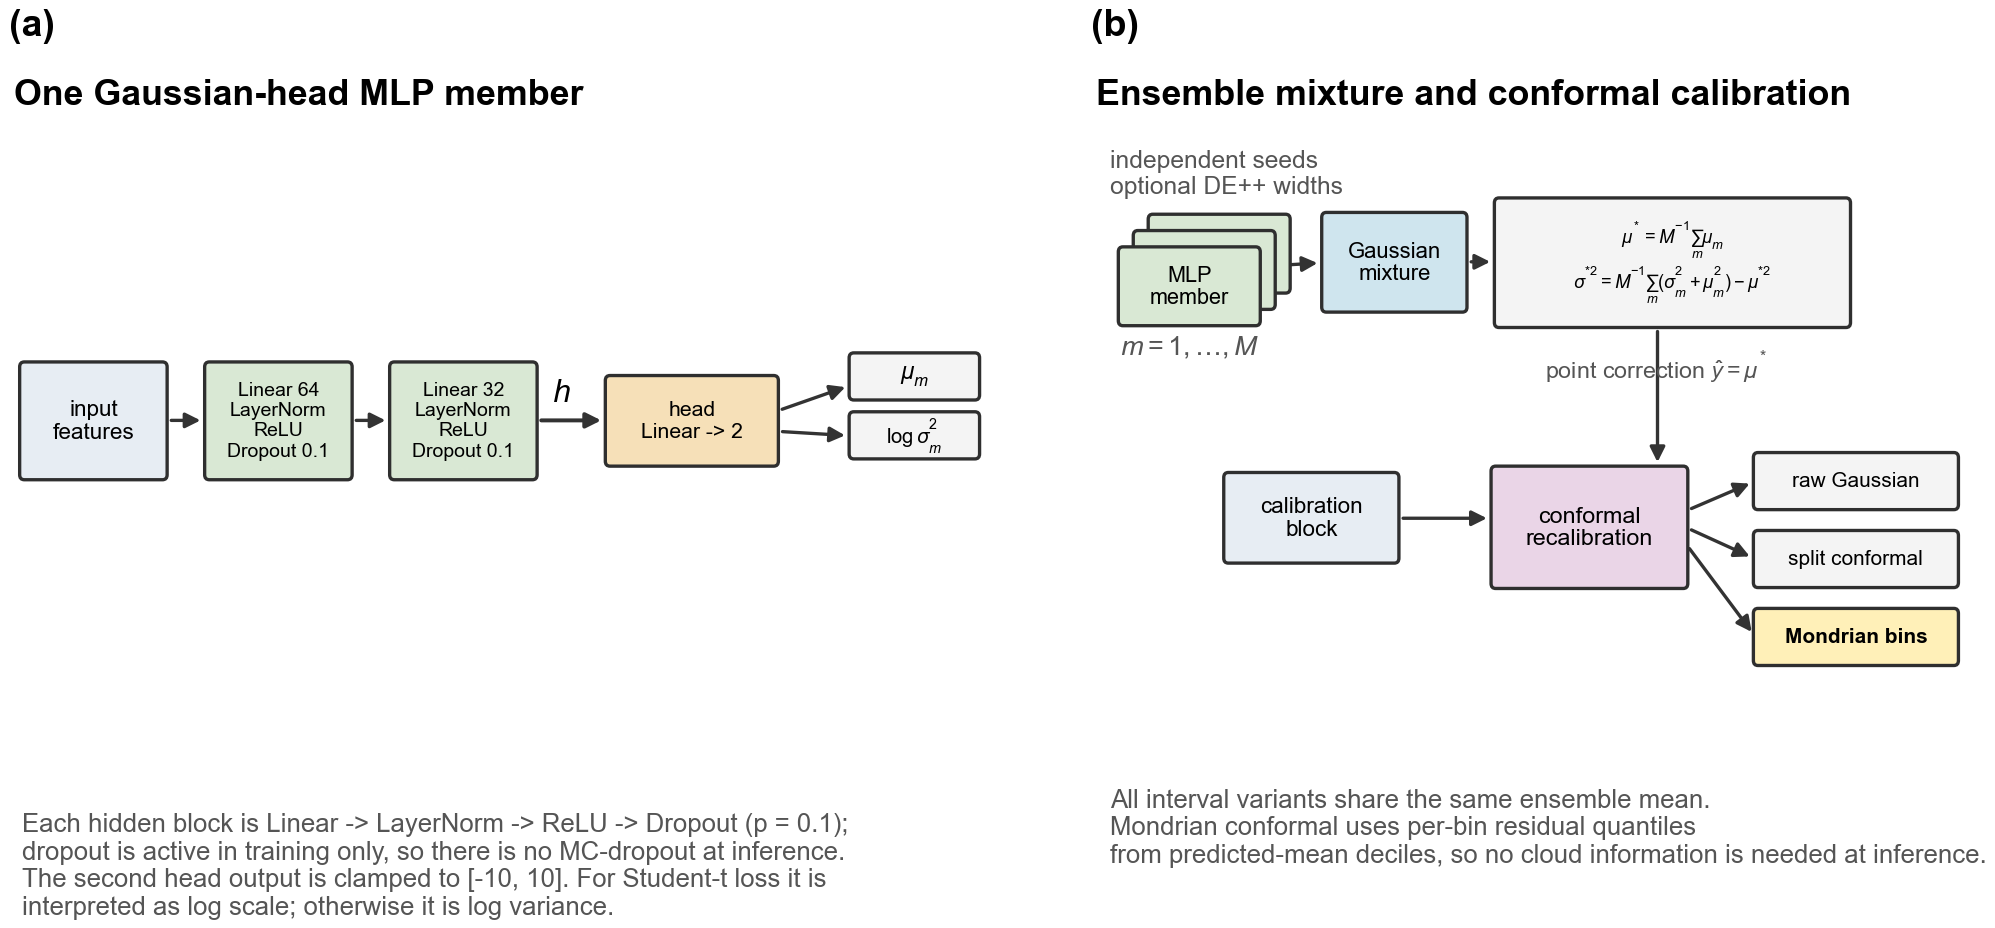
\includegraphics[width=\textwidth]{figures/fig02_deep_ensemble_architecture.png}
\caption{Per-surface probabilistic correction model. (a) One Gaussian-head MLP member (64→32 hidden units; layer normalization and dropout 0.1; $\mu$, $\log{\sigma^2}$ heads; $\beta$-NLL loss, $\beta$ = 0.5). (b) M = 5 members per fold pooled as a Gaussian mixture, followed by split and Mondrian conformal calibration of the 90 \% intervals. All inputs are per-sounding L2 Lite quantities: cloud distance enters only label construction and evaluation — never the model input — so the correction runs footprint-by-footprint with no imager and no along-track context at inference.}
\label{fig:DE_structure}
\end{figure}
%



\subsection{Analysis, training, validation splits, and leakage control}
\label{sec:method-daataset-split}


For the analysis and for training the $\mathrm{X_{CO2}^{B11}}$ bias correction, we use data from the 1st and the 15th of each month (or the closest available date) from 2016 to 2020. Other individual dates from 2014 to 2024 are reserved for validating the correction against $\mathrm{X_{CO2}}$ from TCCON stations, from the ATom airborne campaign, and from two shipborne campaigns. The training and analysis dates are listed in Table~\ref{tab:dates_training}, and the
observation-comparison dates in Table~\ref{tab:dates_comparison}.

The 2016--2020 training and analysis set contains 116 dates. Two months (August
and September 2017) have no usable data, and six nominal dates are replaced by a
neighbouring day where no OCO-2 or MODIS granule is available
(Table~\ref{tab:dates_training}). Across these dates there are $1.05\times10^{7}$
ocean and $7.22\times10^{6}$ land soundings with a valid
$\mathrm{X_{CO2}^{B11}}$, including the nadir, glint, and target modes and both
quality flags 0 and 1. Among them, only $7.85\times10^{6}$ ocean ($74.4\,\%$) and
$3.84\times10^{6}$ land ($53.2\,\%$) soundings have a valid within-orbit anomaly
$\Delta\mathrm{X_{CO2}^{B11}}$; the remaining soundings do not have enough stable,
away-from-cloud reference footprints nearby
(Sect.~\ref{sec:method-cld_dist_xco2_anom}). The lower fraction over land reflects
the smaller number of qualifying reference footprints there. All soundings with a
valid $\Delta\mathrm{X_{CO2}^{B11}}$ are used in the analysis and in the training
(Sect.~\ref{sec:result-cld_dist} and Sect.~\ref{sec:result-spec_anal}).

We split the data by date rather than by sounding, using a five-fold block
rotation. The 116 dates are sorted and partitioned into five contiguous blocks.
Each fold holds out one block ($\sim$24 dates) as the test subset, so every date
serves as a test date exactly once across the five folds. Of the remaining
$\sim$92 dates, $15\,\%$ form the calibration subset and the rest are the
proper-training subset, which gives about $67:12:21$ dates for
training\,:\,calibration\,:\,test. Figure~\ref{fig:5fold_illustration} illustrates
this design. Splitting by date keeps soundings from the same orbit out of two
different subsets, and the contiguous blocks avoid placing adjacent dates in both
the training and the test subsets.

Within each fold, every fitted transform is derived from the proper-training
subset alone. The EOF decomposition of the temperature, water vapour, and
\ce{CO2} profiles is therefore fitted five times, once per fold, and the feature
scaling is fitted the same way. The calibration subset is used only for early
stopping and for the conformal recalibration, and the test subset is used only for
reporting. In this way no information from the calibration dates, the test dates,
or the external validation references enters any fitted transform.



The trained models are then applied to the comparison sets, which comprise 96
TCCON station-days, 8 ATom flight days, and 4 shipborne days
(Table~\ref{tab:dates_comparison}). None of the 82 distinct comparison dates
appears in the training and analysis set.

\subsection{Evaluation framework}
\label{sec:method-eval}

\subsubsection{Predicted $\Delta\mathrm{X_{CO2}^{model}}$ evaluation}
\label{sec:method-eval-del-xco2}

On the test subsets of the training/analysis data, we evaluate each model by how
well its predicted anomaly $\Delta\mathrm{X_{CO2}^{model}}$ reproduces the target
$\Delta\mathrm{X_{CO2}^{B11}}$. We report the date-blocked coefficient of
determination ($R^2$) and root-mean-square error (RMSE) of the predicted versus
target anomaly, together with the per-footprint RMSE and residual scatter. Because
the deep ensemble is probabilistic, we also assess the calibration and the
prediction-interval coverage of its intervals. Statistical significance is
established with paired Wilcoxon signed-rank tests and a site-clustered bootstrap,
and we additionally report a random-effects residual comparison and the
associated representation error.

We evaluate all models under a common protocol: the Ridge and XGBoost baselines,
the TabM and deep-ensemble models, the feature-free within-orbit smoother (a
predictor-free null model), and the feature-set ablations
(Sect.~\ref{sec:...}).


\subsubsection{$\mathrm{X_{CO2}}$ comparison across different products}
\label{sec:method-eval-obs-xco2}

To compare OCO-2 $\mathrm{X_{CO2}}$ ($\mathrm{X_{CO2}^{OCO}}$) with $\mathrm{X_{CO2}}$
from TCCON stations ($\mathrm{X_{CO2}^{TCCON}}$), the ATom airborne campaign
($\mathrm{X_{CO2}^{ATom}}$), and two shipborne campaigns
($\mathrm{X_{CO2}^{ship}}$), we apply product-specific harmonization to reduce the
differences that arise from the different retrieval methods. For the TCCON
comparison, we apply the averaging-kernel (AK) and prior harmonization together
with a wet-to-dry prior conversion, following
\citet{wunch2011tccon_network,das2025oco2_v111_tccon_ggg2020,rodgers2003intercomparison}.
The details of the AK and prior harmonization and of the wet-to-dry conversion are
given in Appendix~\ref{app:ak_operation}.

For the ATom comparison, we build a pseudo-column dry-air $\mathrm{X_{CO2}^{ATom}}$
from the in-situ \ce{CO2} profiles measured by the aircraft.

For the shipborne measurements, the averaging kernel and prior they used are not
available, so we compare $\mathrm{X_{CO2}^{OCO}}$ with $\mathrm{X_{CO2}^{ship}}$
directly. The residual product-level difference may therefore be larger for the
shipborne comparison.

We set the collocation search radius between the TCCON station, the ATom
pseudo-column center, or the ship-track center and the OCO-2 soundings to
$100$~km, and the temporal search window to $\pm1$~h around the OCO-2 overpass.
The $\pm1$~h window is the same as \citet{das2025oco2_v111_tccon_ggg2020}, while
our spatial window is stricter than their default coincidence box of
$2.5^\circ \times 5^\circ$ in latitude--longitude centred on the station
($\pm1.25^\circ$ latitude, corresponding to about $139$~km, and $\pm2.5^\circ$
longitude); they tighten the box only at a few sites affected by local pollution
or terrain. Unlike their analysis, which uses only good-quality soundings
(\texttt{xco2\_quality\_flag}~$=0$) and compares the median of each overpass, we
include both quality flags (0 and 1) and evaluate the comparison at the
individual footprint level, which is necessary to resolve the near-cloud
behavior that is the subject of this study.

For each station-day $s$ (one TCCON site on one overpass date) with $n_s$
collocated soundings, let
$e_{s,i} = X_{\mathrm{CO2},i} - X^{\mathrm{TCCON}}_{\mathrm{CO2},i}$
denote the footprint residual against the AK-harmonised TCCON reference,
evaluated once for the uncorrected product and once after correction. The
station-day mean bias and per-footprint root-mean-square error are
\begin{equation}
  b_s \;=\; \frac{1}{n_s}\sum_{i=1}^{n_s} e_{s,i},
  \qquad
  R_s \;=\; \Bigl(\frac{1}{n_s}\sum_{i=1}^{n_s} e_{s,i}^{2}\Bigr)^{1/2}.
\end{equation}
Figure~8a (Results 4.4) summarises the $S = 75$ station-days by three aggregates:
the station-day-equal mean absolute bias
$\overline{|b|} = S^{-1}\sum_s |b_s|$, which weights every station-day
equally regardless of its footprint count; the root-mean-square bias
$\mathrm{RMS}_b = (S^{-1}\sum_s b_s^{2})^{1/2}$, a quadratic aggregate of
the same station-day mean biases that emphasizes the largest-bias
station-days (it is not a footprint-level error metric); and the mean
per-footprint RMSE $\overline{R} = S^{-1}\sum_s R_s$, which measures
footprint-level scatter about the reference. Each row of Fig.~8a shows
the change $\Delta$ (corrected $-$ uncorrected) of one aggregate, so
negative values are improvements: $\overline{|b|}$ and $\mathrm{RMS}_b$
respond only to systematic station-day offsets, whereas $\overline{R}$
also responds to within-overpass scatter. Confidence intervals and
$p$-values come from a site-clustered bootstrap: the 18 sites are
resampled with replacement, each drawn site contributing all of its
station-days ($B = 10\,000$ resamples), which respects the strong
within-site clustering of the sample (e.g.\ R\'eunion contributes 14
station-days); the interval is the 2.5--97.5 percentile range of the
resampled $\Delta$, and the two-sided
$p = 2\min[P(\Delta \ge 0),\, P(\Delta \le 0)]$, floored at
$2/(B+1)$. The paired Wilcoxon test quoted beneath the panel treats
station-days as exchangeable pairs and is reported as a
clustering-agnostic cross-check.

% \subsection{Safety and robustness experiments}
\label{sec:method-safety-exp}


After the \emph{DE-MLP} model is trained, we test the impact of \emph{DE-MLP} model correction on various scenarios. The far-cloud and clear-day footprints negative controls versus the TCCON observations are analyzed. We also test the potential plume-removal issue of emission sources. Other tests includes target-radius and TCCON-coincidence sensitivity, 

Describe without reporting outcomes:

- far-cloud and clear-day negative controls;
- Nassar power-plant transects and matched control windows;
- spectral-channel plume-removal bounds;
- target-radius and TCCON-coincidence sensitivity;
- raw versus operational-BC versus ML comparison;
- surface and environmental failure-mode stratification.

\section{Results}

\subsection{Cloud-proximity phenomenology}
\label{sec:result-cld_dist}

% Lead with the observation:

% - XCO2 anomaly versus cloud distance;
% - positive near-cloud response over land and negative response over ocean;
% - characteristic land-r15 and ocean-r05 distance scales;
% - quality-flag composition and observation loss with cloud distance.

% This result establishes the problem before introducing correction skill.

We analyze the $17.75$M footprints from the 2016-2020 analysis set (Sect.~\ref{sec:method-daataset-split}) with a valid nearest cloud distance. $41.7\%$ of all footprints lie within 4 km of the nearest detected cloud ($60.7\%$ within 10 km). We use $d_0 = 10$~km as the reference to calculate the \xcobc anomaly ($\Delta \mathrm{X_{CO2}^{B11}}$), as shown in Fig.~\ref{fig:OCO-ocean-land-cld_dist}a. The results demonstrate that $\Delta \mathrm{X_{CO2}^{B11}}$ is opposite in sign, with negative over ocean and positive over land before any correction is applied. Furthermore, the ocean response has decayed by $\thicksim5$ km, well inside the threshold, whereas the land response is still $\thicksim0.5$ ppm when the 10-km reference cut truncates it by construction. In other words, the cloud-influence distance could be different over ocean and land. As a result, we set the new reference distances separately with $d_0 = 5$~km for ocean and $d_0 = 15$~km for land.



\begin{figure}[t]
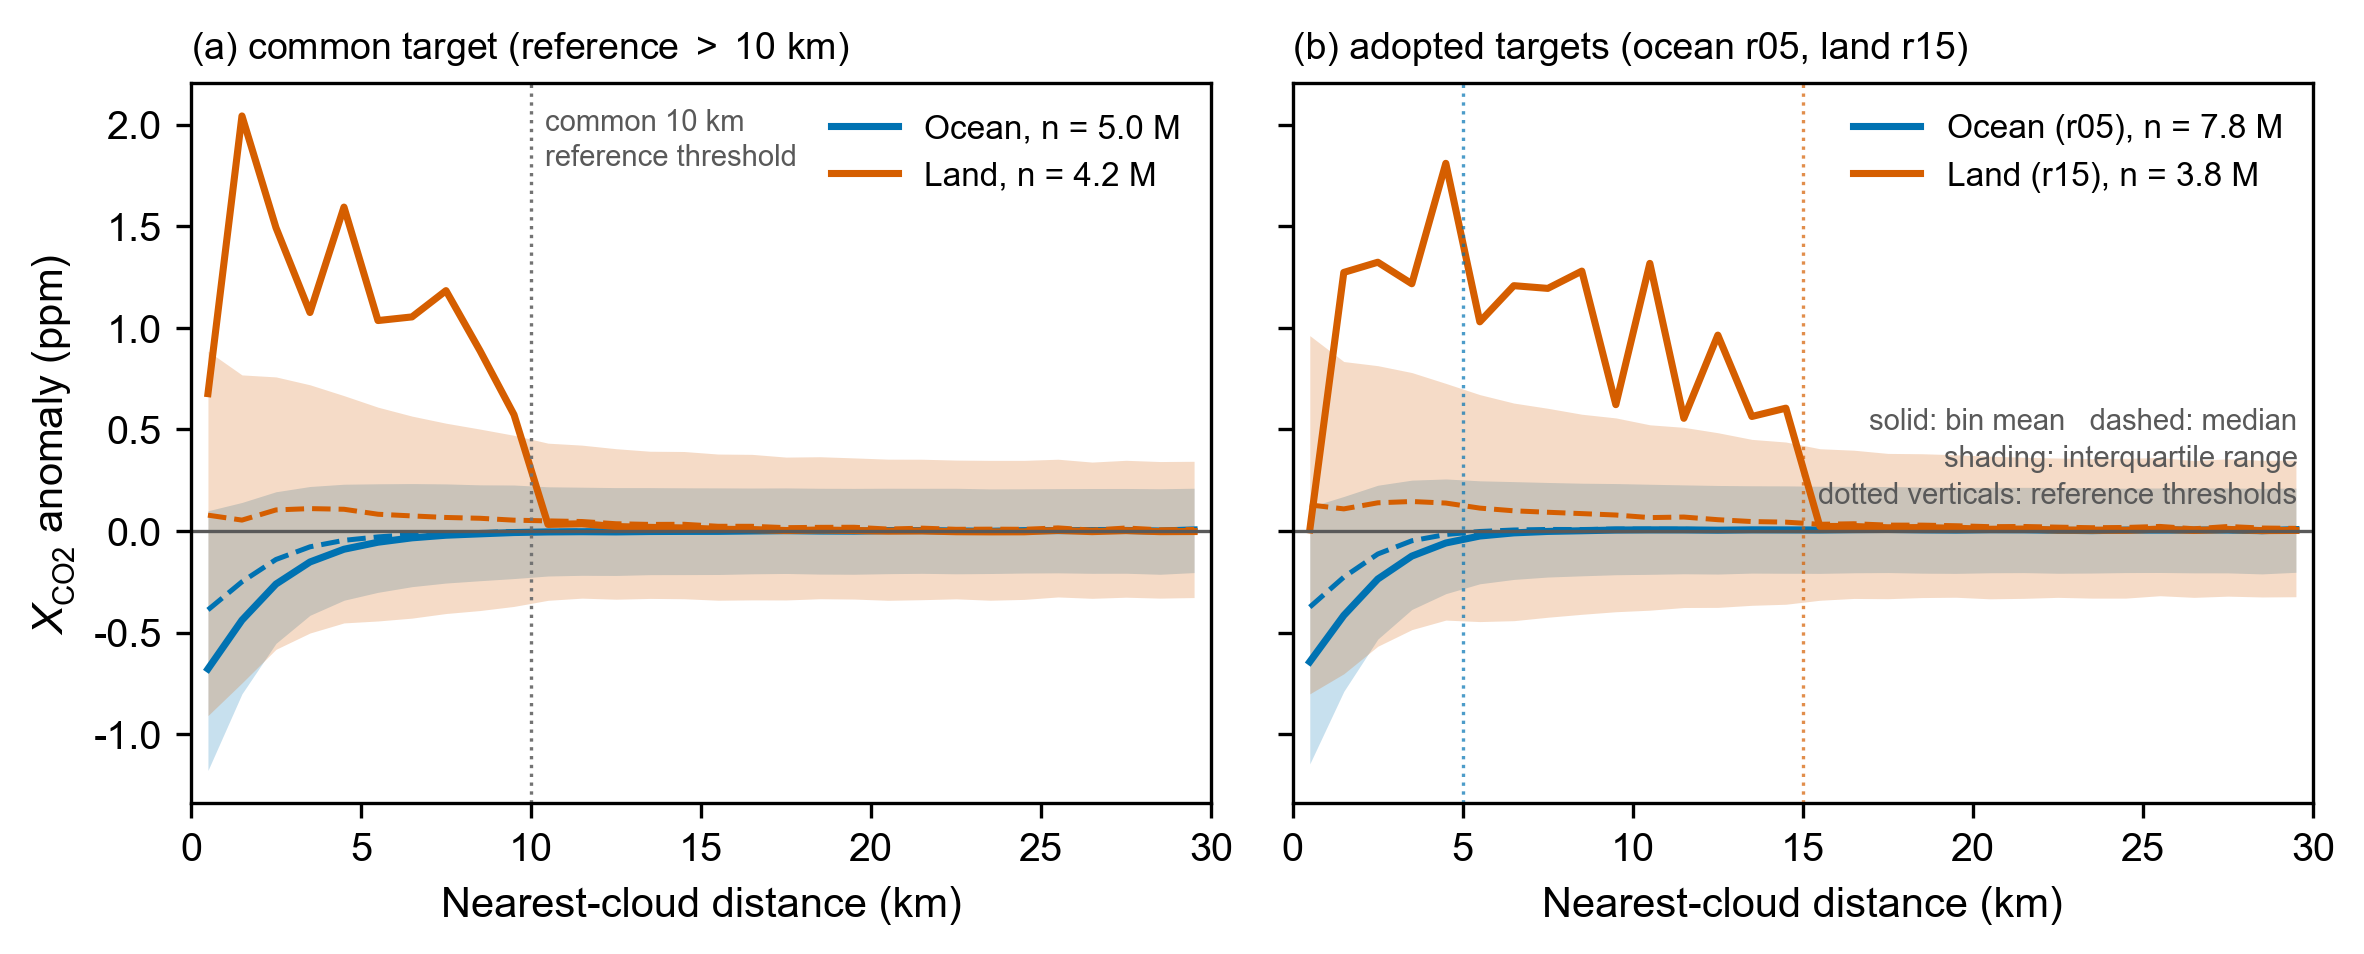
\includegraphics[width=\textwidth]{figures/fig03_anomaly_decay.png}
\caption{Within-orbit clear-sky \xco anomaly versus nearest-cloud distance for the 2016–2020 analysis set (116 dates; 1-km bins). (a) Both surfaces under a common anomaly target whose clear-sky reference lies beyond 10 km. The common threshold is too tight for land and unnecessarily wide for ocean, motivating the surface-specific radii. (b) The adopted production targets with ocean referenced beyond 5 km (r05, n = 7.8 M) and land beyond 15 km (r15, n = 3.8 M). Solid lines show the bin mean, dashed lines the median, and shading the interquartile range: over ocean the whole distribution shifts negative near cloud, whereas over land the mean far exceeds the nearly unmoved median. The land bias is carried by a skewed tail of strongly affected soundings rather than a shift of the full population.}
\label{fig:OCO-ocean-land-cld_dist}
\end{figure}


After recalculating $\Delta \mathrm{X_{CO2}^{B11}}$, the land response indeed persists to $\thicksim15$ km, and the ocean curve is unchanged (Fig.~\ref{fig:OCO-ocean-land-cld_dist}b). The dotted lines mark each reference threshold, beyond which the anomaly returns to zero by construction. The signature of opposite sign of ocean and land $\Delta \mathrm{X_{CO2}^{B11}}$ also remains the same. 59.1\% of ocean footprints are within the 5 km ocean target radius, and 46.8\% of land footprints are within the 15 km land target radius. We use the newly calculated $\Delta \mathrm{X_{CO2}^{B11}}$ with $r05$ for ocean and $r15$ for land in later analysis and training.

\subsection{Spectral features and cloud distance}
\label{sec:result-spec_anal}


We derive the spectral features by fitting from three OCO-2 bands, as described in Sect.~\ref{sec:methods_photon_path}. The land footprints are categorized as various surface types based on the MODIS yearly land cover type product (MCD12C1). We compare the average difference of each variable from near-cloud and far-cloud footprints (nearest cloud distance < $5$~km for ocean and <$15$~km for land). For each surface class $g$ and reference-corrected spectral variable
$\Delta v$, the near-cloud effect size shown in Fig.~\ref{fig:land_type_features} is the
far-field-normalized difference
%
\begin{equation}
  E_z(\Delta v, g) \;=\;
  \frac{\overline{\Delta v}_{g}^{\,\mathrm{near}}
       - \overline{\Delta v}_{g}^{\,\mathrm{far}}}
       {\sigma_{g}^{\mathrm{far}}(\Delta v)} ,
  \label{eq:effect-size}
\end{equation}
%
where $\Delta v_i = v_i - \bar{v}_i^{\mathrm{ref}}$ is the per-sounding departure of $v \in \{\langle l'\rangle, \mathrm{var}(l'), \text{exp-intercept}\}$ (per band) from the mean over the same-orbit clear-sky reference population of the surface-specific production target (cloud distance $> 5$\,km over ocean
and $> 15$~km over land, within $\pm 0.25^{\circ}$ latitude), the near and far windows are 0--5\,km and $20$--$50$~km of nearest-cloud distance, which are identical for every class, ocean included, so all cells are directly comparable (the far window lies beyond the response scale of both surfaces, and the near window contains the full ocean response and the strongest part of the land response). The $\sigma_{g}^{\mathrm{far}}$ is the standard deviation of $\Delta v$ in the far window of class $g$, so that $E_z$ reads as the number of far-field standard deviations by which the class
moves near cloud. The analytic 95\,\% confidence interval is $1.96\,[(\mathrm{SE}^{\mathrm{near}})^2 +
(\mathrm{SE}^{\mathrm{far}})^2]^{1/2} / \sigma_{g}^{\mathrm{far}}$;
asterisks in Fig.~\ref{fig:land_type_features} mark cells with $|E_z|$ exceeding this interval. Only
operational quality flag (xco2\_quality\_flag; QF) of 0, snow-free soundings enter. We also exclude cells with fewer than 500 soundings in either window. Because the path-length features derive from the L1B radiances, the QF has no mechanical connection to them; its role here is to define the physical population, since the flag rate is both distance-dependent (rising toward cloud) and class-dependent, and flagged scenes carry competing scattering perturbations (in-field-of-view cloud, aerosol) that are not the clear-scene proximity effect under study. The surface-specific reference radii match the production anomaly targets of Sect.~\ref{sec:result-cld_dist} ($5$~km for ocean and $15$~km for land).




The sign of the W\ce{CO2} $\Delta$ ⟨$l′$⟩ response follows the sign of the cloud−surface albedo contrast across the full surface axis of Fig.~\ref{fig:land_type_features}. It is positive over dark ocean (+0.09$\sigma$) and vegetated classes (savanna +0.48σ), negative over bright barren surfaces (−1.29$\sigma$). Magnitudes do not rank with contrast, so the albedo-contrast mechanism enters as a sign rule. The sparse urban class is thin and is not interpreted. The continuum-reflectance response ($\Delta$ exp-int) is strongly negative over ocean, consistent with shadow-dominated darkening of the dark surface. The shadow and brightening branches of Fig.~{fig:shadow-brightening} carry opposite-signed \xco anomalies and distinct band-resolved $\Delta$ ⟨$l′$⟩ responses, and are separable from a single footprint's spectrum alone.


Repeating the analysis on QF=1 and QF=0 and 1 populations (Appendix B, Fig. B4) leaves the sign of every ocean and vegetated-class cell unchanged. The single exception is barren, where 67\% of soundings are flagged (desert dust and bright-scene retrieval failures), and the QF=1 population responds *positively* toward the cloud signature,  diluting the clear-scene response (−1.29$\sigma$) to −0.23$\sigma$ when all flags are pooled. This flip corroborates rather than weakens the sign rule. It is consistent with the features responding to in-scene scattering contamination itself, uniformly positive across all surfaces, while the quality-filtered population isolates the clear-scene albedo-contrast response. The QF=0 estimates are conservative, since near-cloud soundings that survive the filter are the least-perturbed scenes.



\begin{figure}[t]
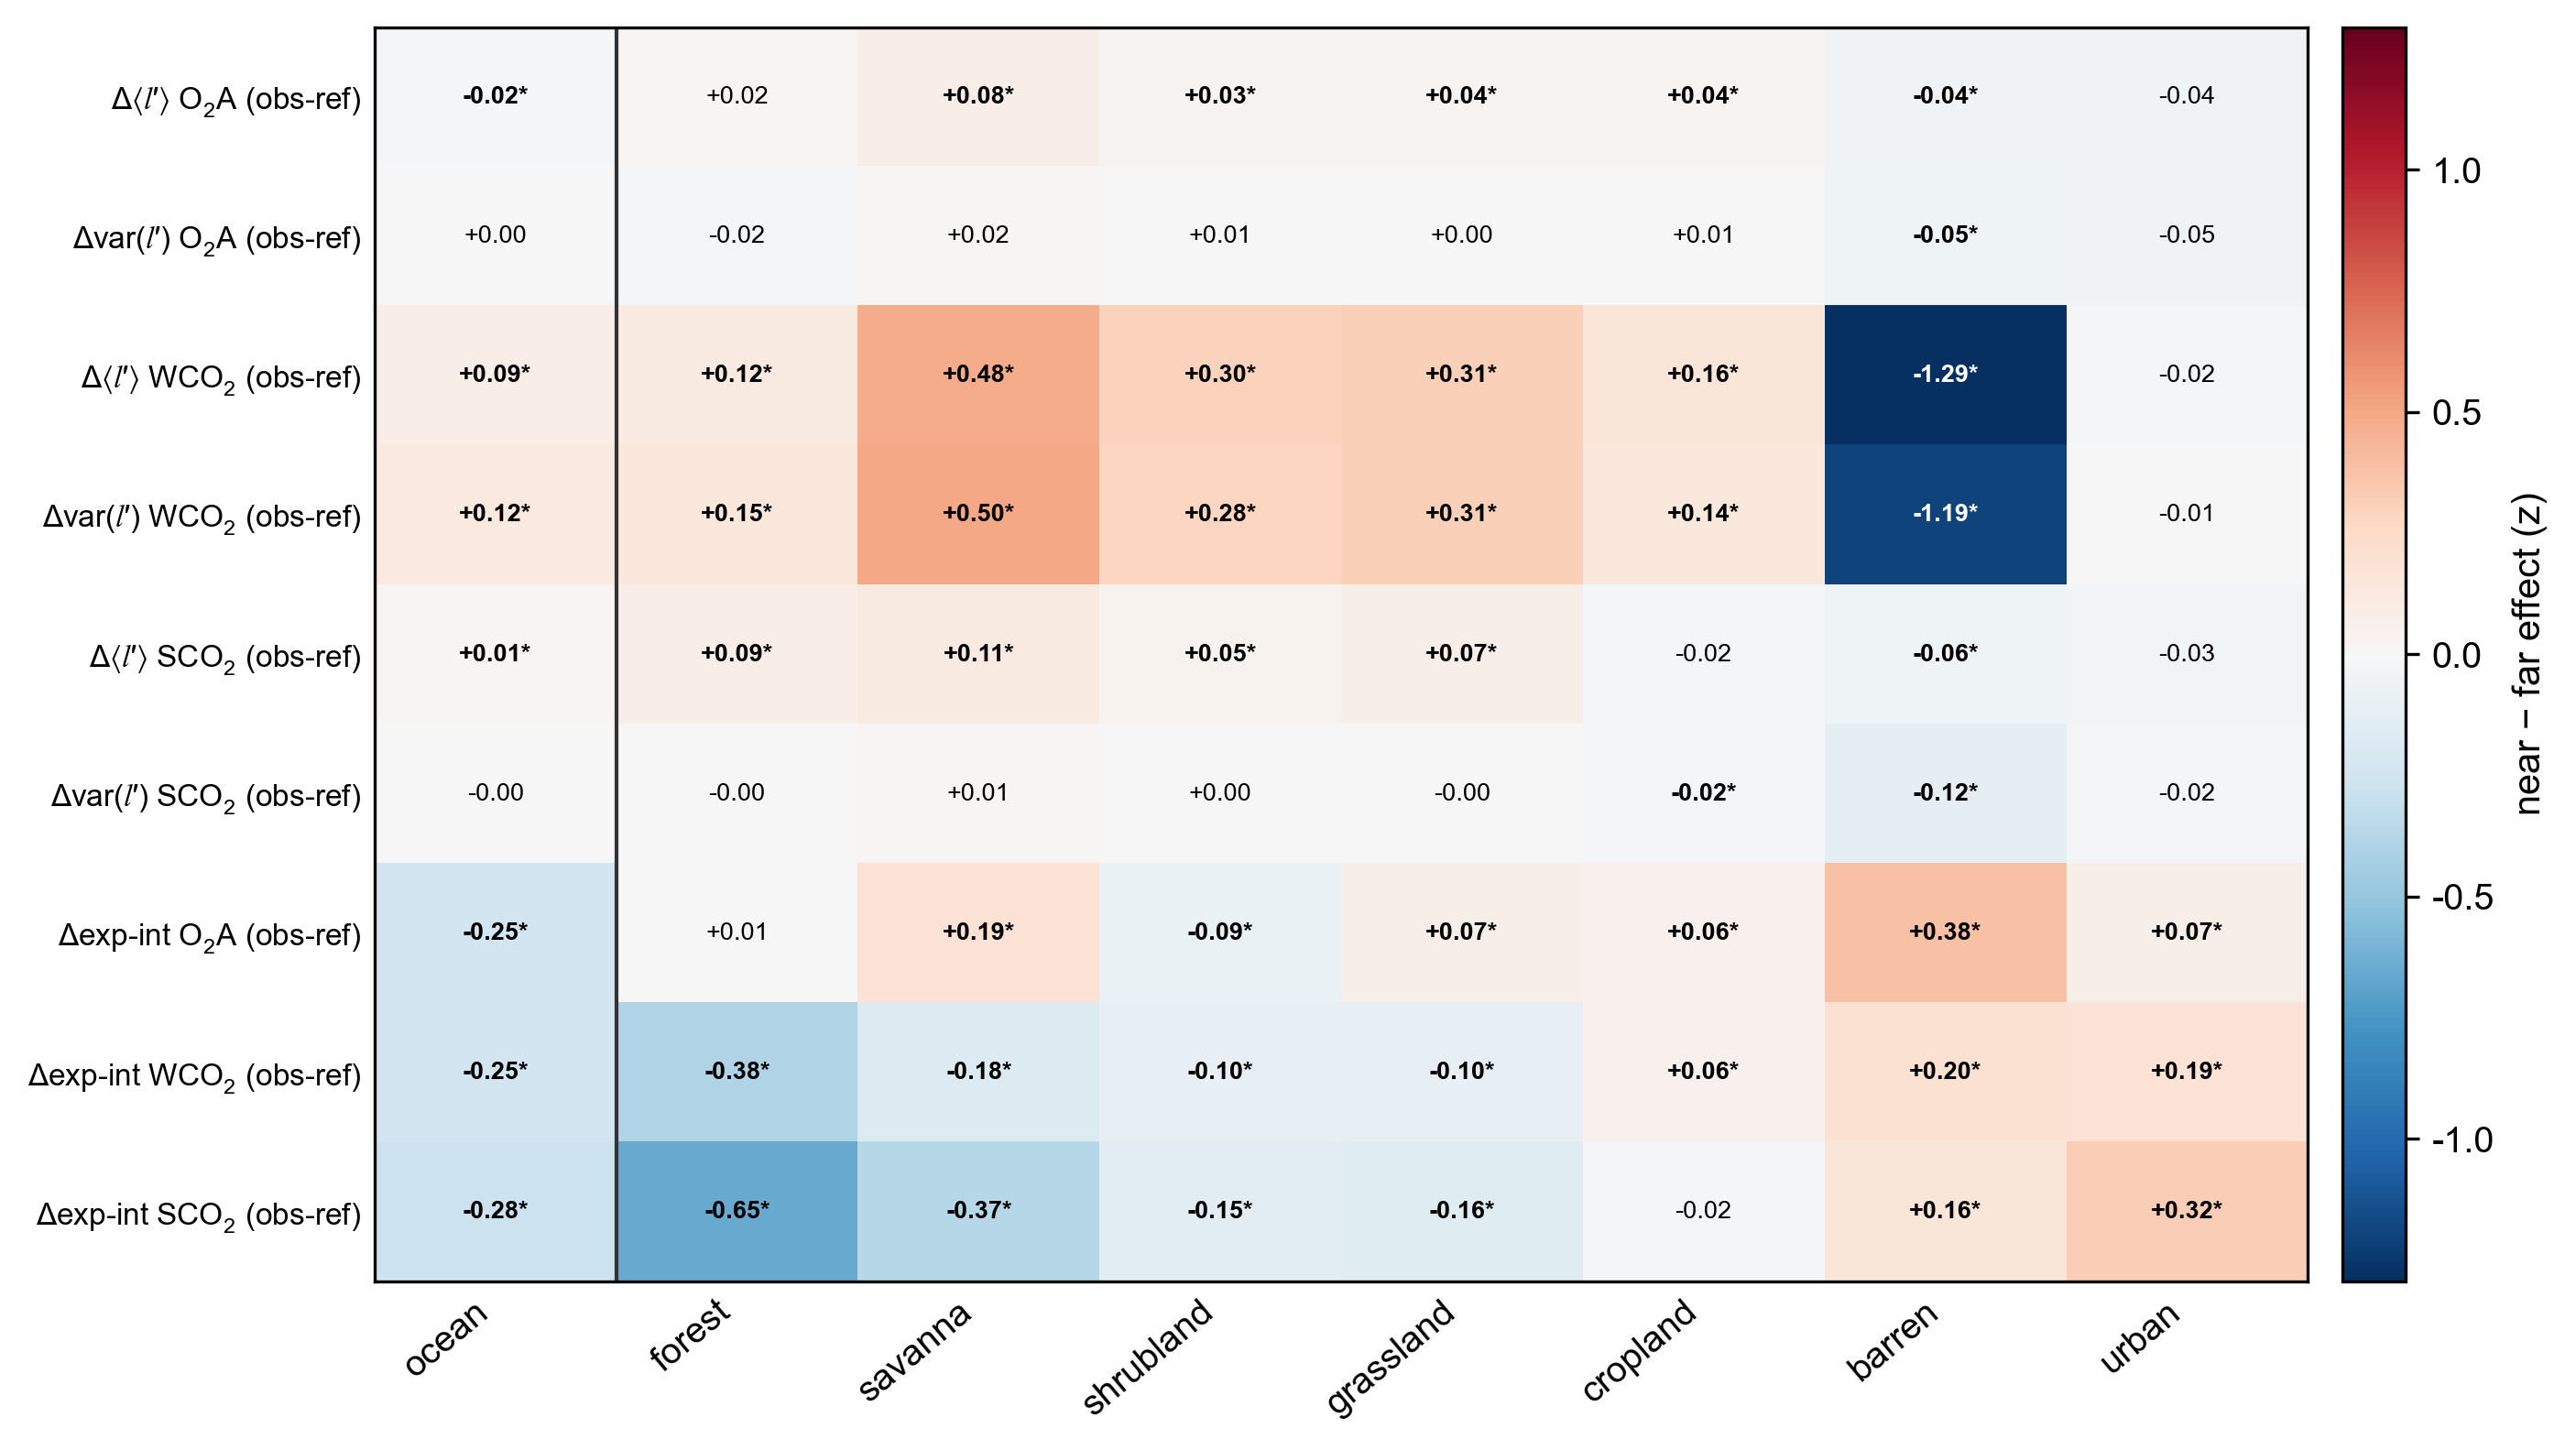
\includegraphics[width=\textwidth]{figures/fig04_landclass_effect_heatmap.png}
\caption{Surface-stratified near-cloud spectral response of effect size (Eq. \ref{eq:effect-size}; near-cloud 0–5 km minus far-cloud 20–50 km, in far-field standard deviations) of the reference-corrected path-length features for ocean and for each MCD12C1 land-cover class. Quality-flag-0, snow-free soundings; per-sounding references use the surface-specific clear-sky radii of the production targets (ocean beyond 5 km, land beyond 15 km); asterisks mark effects exceeding their analytic 95 \% confidence interval. ⟨$l′$⟩ and var($l'$) are the fitted mean and variance of the relative photon path (the cumulants k1, k2 of Sect. 3.2). Reference and quality-flag sensitivity variants: Appendix B.}
\label{fig:land_type_features}
\end{figure}




\begin{figure}[t]
\centering
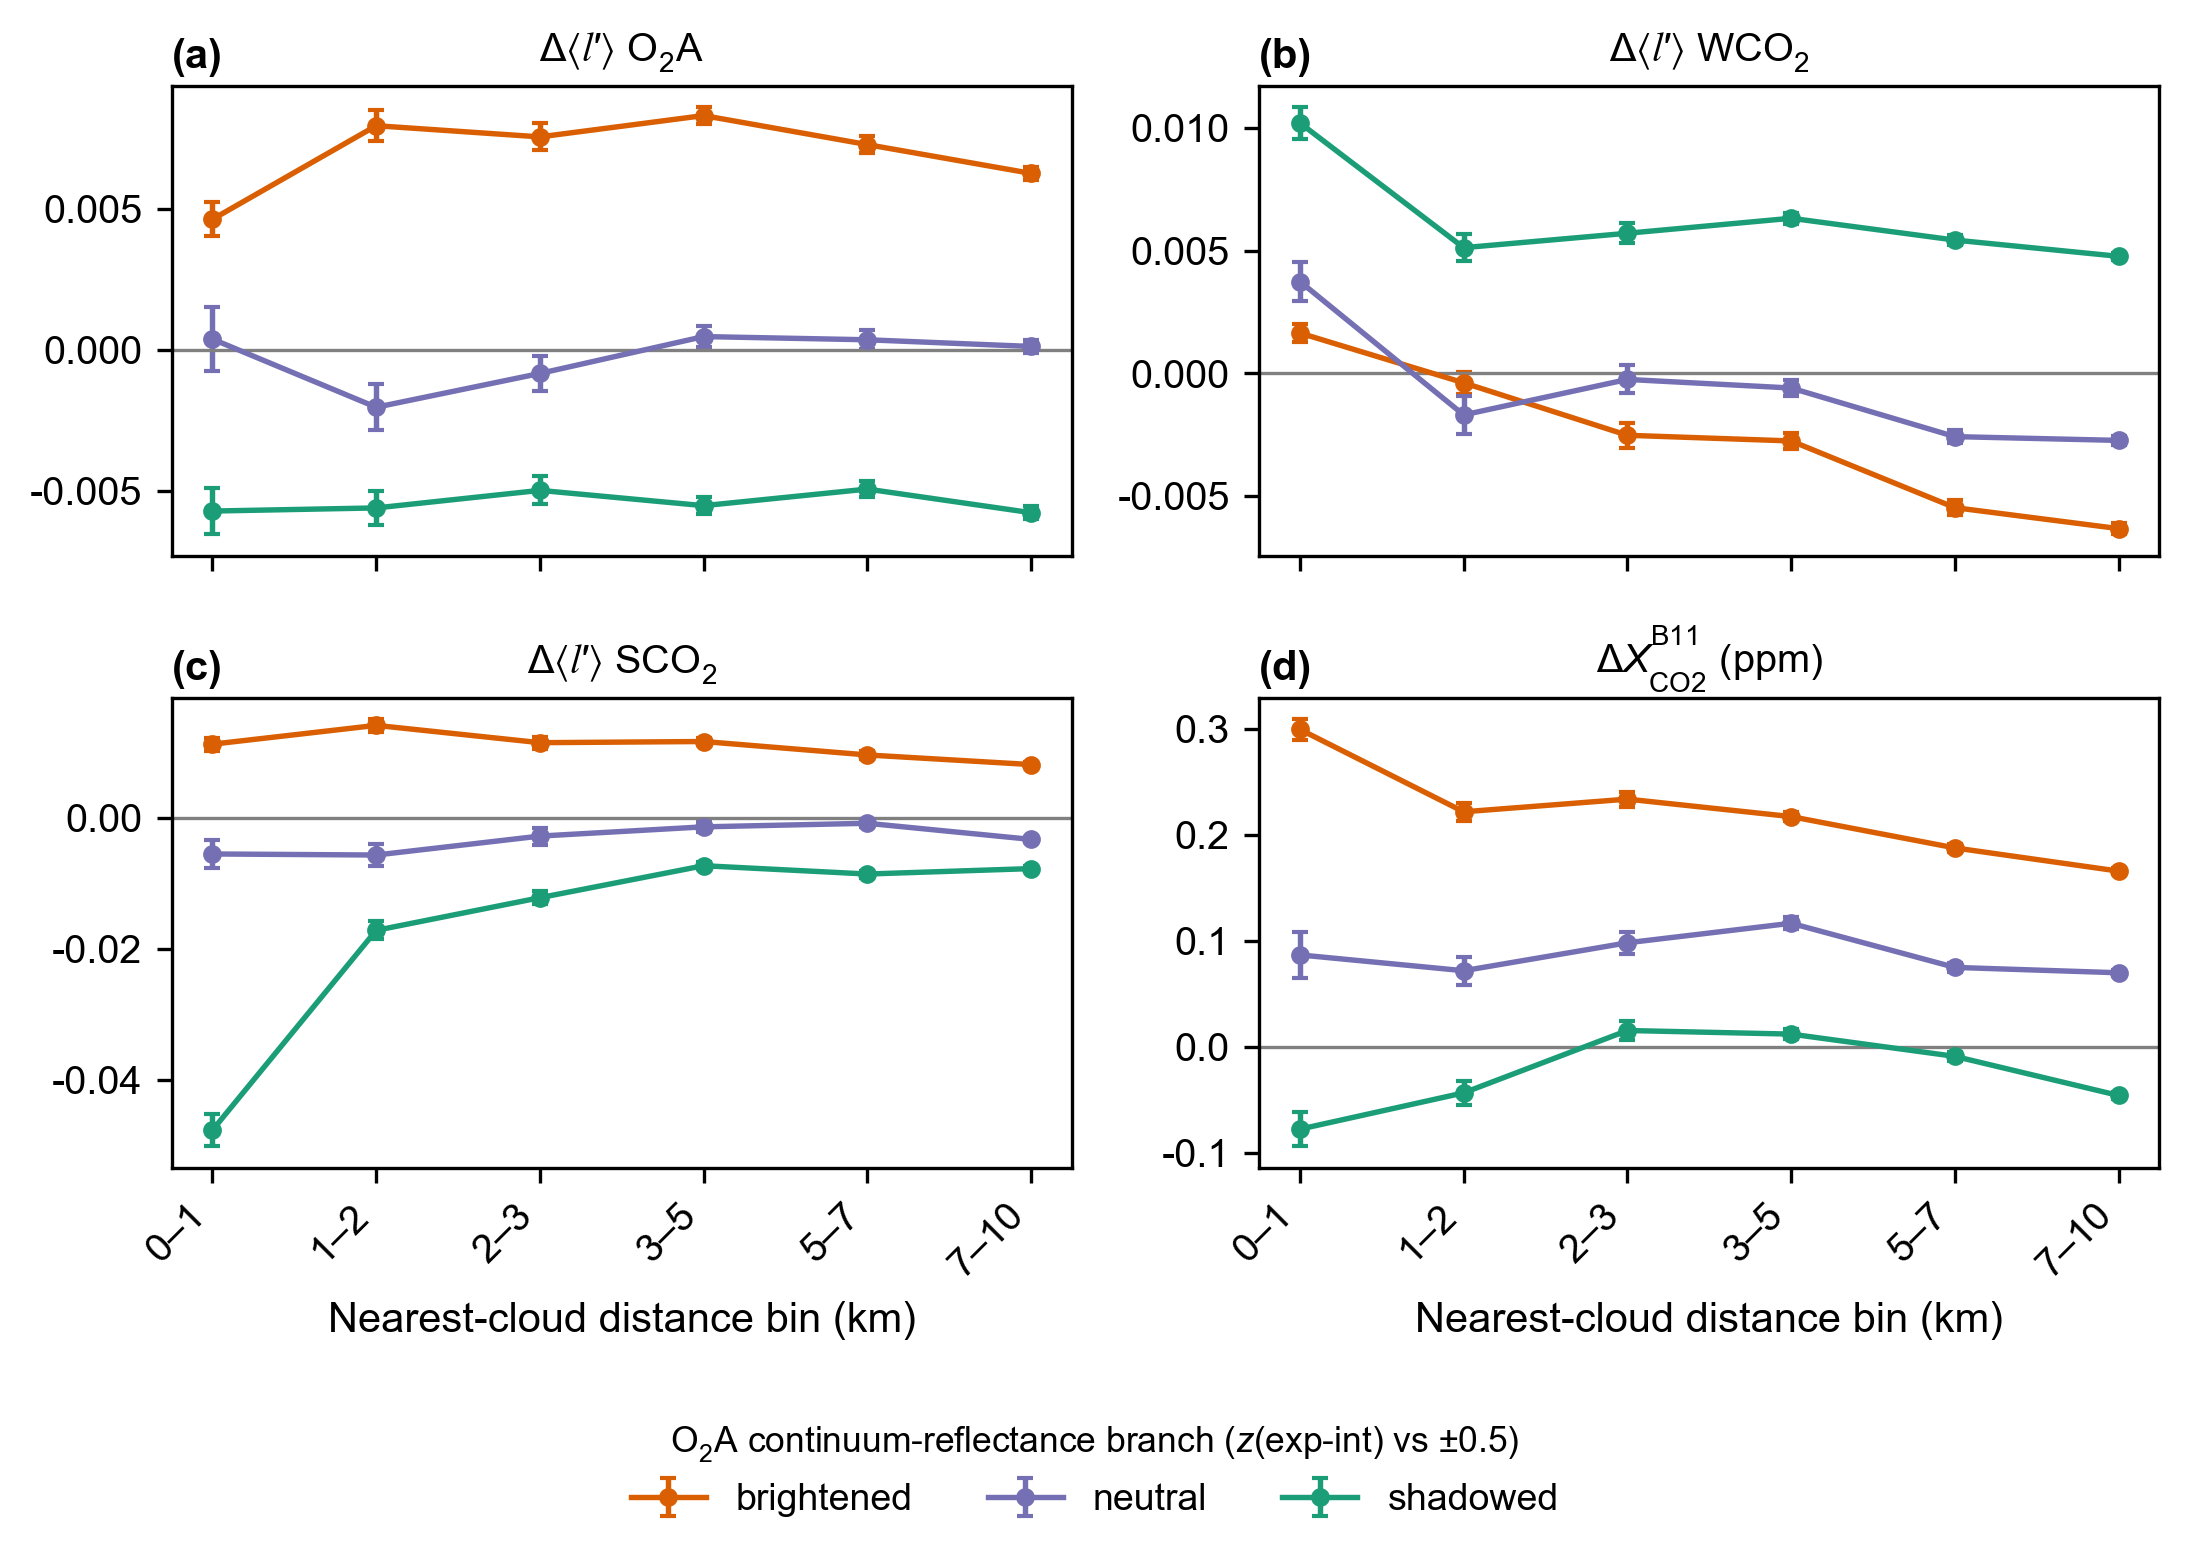
\includegraphics[width=0.8\textwidth]{figures/fig05_shadow_brightening_land.png}
\caption{Shadowing versus brightening. Near-cloud land footprints split by the sign of the \ce{O2}A continuum-reflectance departure from the clear-sky reference (exp-intercept low: cloud shadowing; high: side illumination/brightening), with each branch's \xco anomaly and band-resolved $\Delta$ ⟨$l′$⟩ response. (A single-overpass illustration against Aqua-MODIS true-colour imagery: Appendix G, Fig. G1.)}
\label{fig:shadow-brightening}
\end{figure}




\FloatBarrier

\subsection{Model comparison and feature attribution}
\label{sec:result-model_comp}


The trained \emph{Ridge}, \emph{XGBoost}, and \emph{DE} models with structures and training details in Sect.~\ref{sec:methods-models,sec:method-daataset-split} are compared for their performance over withheld test data and corrected real OCO-2 data. We use ocean and land footprints from the training set to train separate models for ocean and land for all structures. Each model has $5$ members, which are trained on different folds of data (Fig.~\ref{fig:5fold_illustration}). Table~\ref{tab:cv-model-comparison} shows the performance of three models on the same held-out test data. The \emph{DE} has the lowest $RMSE$ and highest $R^2$ when comparing the predicted and true $\Delta$\xcobc, which is better than the \emph{XGBoost} and \emph{Ridge} baselines.


In addition to the $5$ folds held-out test data, we also compare their performance on corrected \xco, which is calculated by
%
\begin{equation}
  \mathrm{X_{CO2}^{model}} = \mathrm{X_{CO2}^{B11}} - \Delta \mathrm{X_{CO2}^{predicted}},
  \label{eq:xco2_corr}
\end{equation}
%
which $\Delta \mathrm{X_{CO2}^{predicted}}$ is predicted \xco anomaly, and $\mathrm{X_{CO2}^{model}}$ is the corrected \xco from different models. The \xcobc, $\mathrm{X_{CO2}^{Ridge}}$, $\mathrm{X_{CO2}^{XGBoost}}$, and $\mathrm{X_{CO2}^{DE}}$ are compared with TCCON measurements following the evaluation method described in Sect.~{sec:method-eval}. Similar to the results of $5$ folds held-out test data, the \emph{DE} model leads at every slice, and the model performance difference is larger in the near-cloud land tail (Fig.~\ref{fig:model_baseline_ablation}a). Though the difference is smaller in the near-cloud ocean tail, the \emph{DE} model still performs better if we consider both the near-cloud ocean tail and QF1 footprints. 

The same ordering holds on the withheld date-blocked folds of the anomaly target (Appendix~\ref{app:model_compare}, Fig.~\ref{fig:model_cv_compare}). The agreement between internal held-out and the independent validations means neither the target construction nor the TCCON chain is driving the selection. Though the fold metrics understate the gap, since the \emph{XGBOOSt} model trails the \emph{DE} model by only ~0.02–0.04 ppm in fold RMSE but by 0.25 ppm on the near-cloud land (≤15 km) TCCON tail. As a result, the \emph{DE} model is used in the later analysis.


After testing the performance over withheld test data and corrected real OCO-2 data, we are interested in the contribution of the feature groups and individual features. We first test removing (1) retrieval-state feature (\xcoraw − \xcoprior), (2) spectral path-length features, and (3) contamination features (See detailed features in Table~\ref{tab:training-config}). As shown in Fig.~\ref{fig:model_baseline_ablation}b, dropping the spectral or contamination groups is TCCON-neutral, whereas removing the retrieval-state departure \xcoraw − \xcoprior) costs 0.8–1.2 ppm. Although using "\xcoraw − \xcoprior" as a feature is similar to looking for an answer of $\Delta$ \xcobc, the $R^2$ between "\xcoraw − \xcoprior" and $\Delta$ \xcobc is only 0.323 for ocean and 0.191 for land. In other words, "\xcoraw − \xcoprior" carries the most abundant cloud-induced \xco bias information, but does not directly reflect the $\Delta$ \xcobc. Even "\xcoraw − \xcoprior" is the most important feature compared to spectral path-length and contamination feature groups, dropping "\xcoraw − \xcoprior" with either spectral path-length or contamination feature groups can degrade the $\Delta \mathrm{RMSE}$ more than not using "\xcoraw − \xcoprior" itself. In particular, dropping "\xcoraw − \xcoprior" with spectral-fitting features shows the largest $\Delta \mathrm{RMSE}$ increase for pooled, near-cloud land and near-cloud ocean tests.


Although the spectral path-length group seems to contribute less than "\xcoraw − \xcoprior" alone, its value lies in three roles "\xcoraw − \xcoprior" cannot fill. First, it indicates the mechanism of cloud-induced bias. The sign rule and shadow/brightening branches of Sect.~\ref{sec:result-spec_anal} establish that the corrected signal is a photon path-length effect, which is something the retrieval-state channel exploits but cannot demonstrate. Second, the spectral path-length group increases the safety of over-correction. The band-resolved fingerprint of Sect.~\ref{sec:result-plume} bounds what the correction may remove. The channel attribution shows the full model removes 55 \% (40–63 \%) of plume-free local clear-sky spread, the no-spectral variant removes 54 \% (the cumulants contribute none of the smoothing essentially), and the no-retrieval-state variant removes 29 \%. The local smoothing flows through the retrieval-state channel while the spectral channel supplies the plume-versus-cloud discriminator. Third, this feature group provides the robustness of imager-independent correction. The cloud-proximity sensitivity of the spectra, including below the MODIS resolution floor (Supplement S4), is what makes imager-free deployment and cross-sensor transfer (Sect.~\ref{sec:disc-img-free}, Appendix H) conceivable. In short, the spectral path-length features establish what the bias is and bound what the correction may touch, while the retrieval-state feature is the operationally sufficient predictor of it.






\begin{figure}[t]
\centering
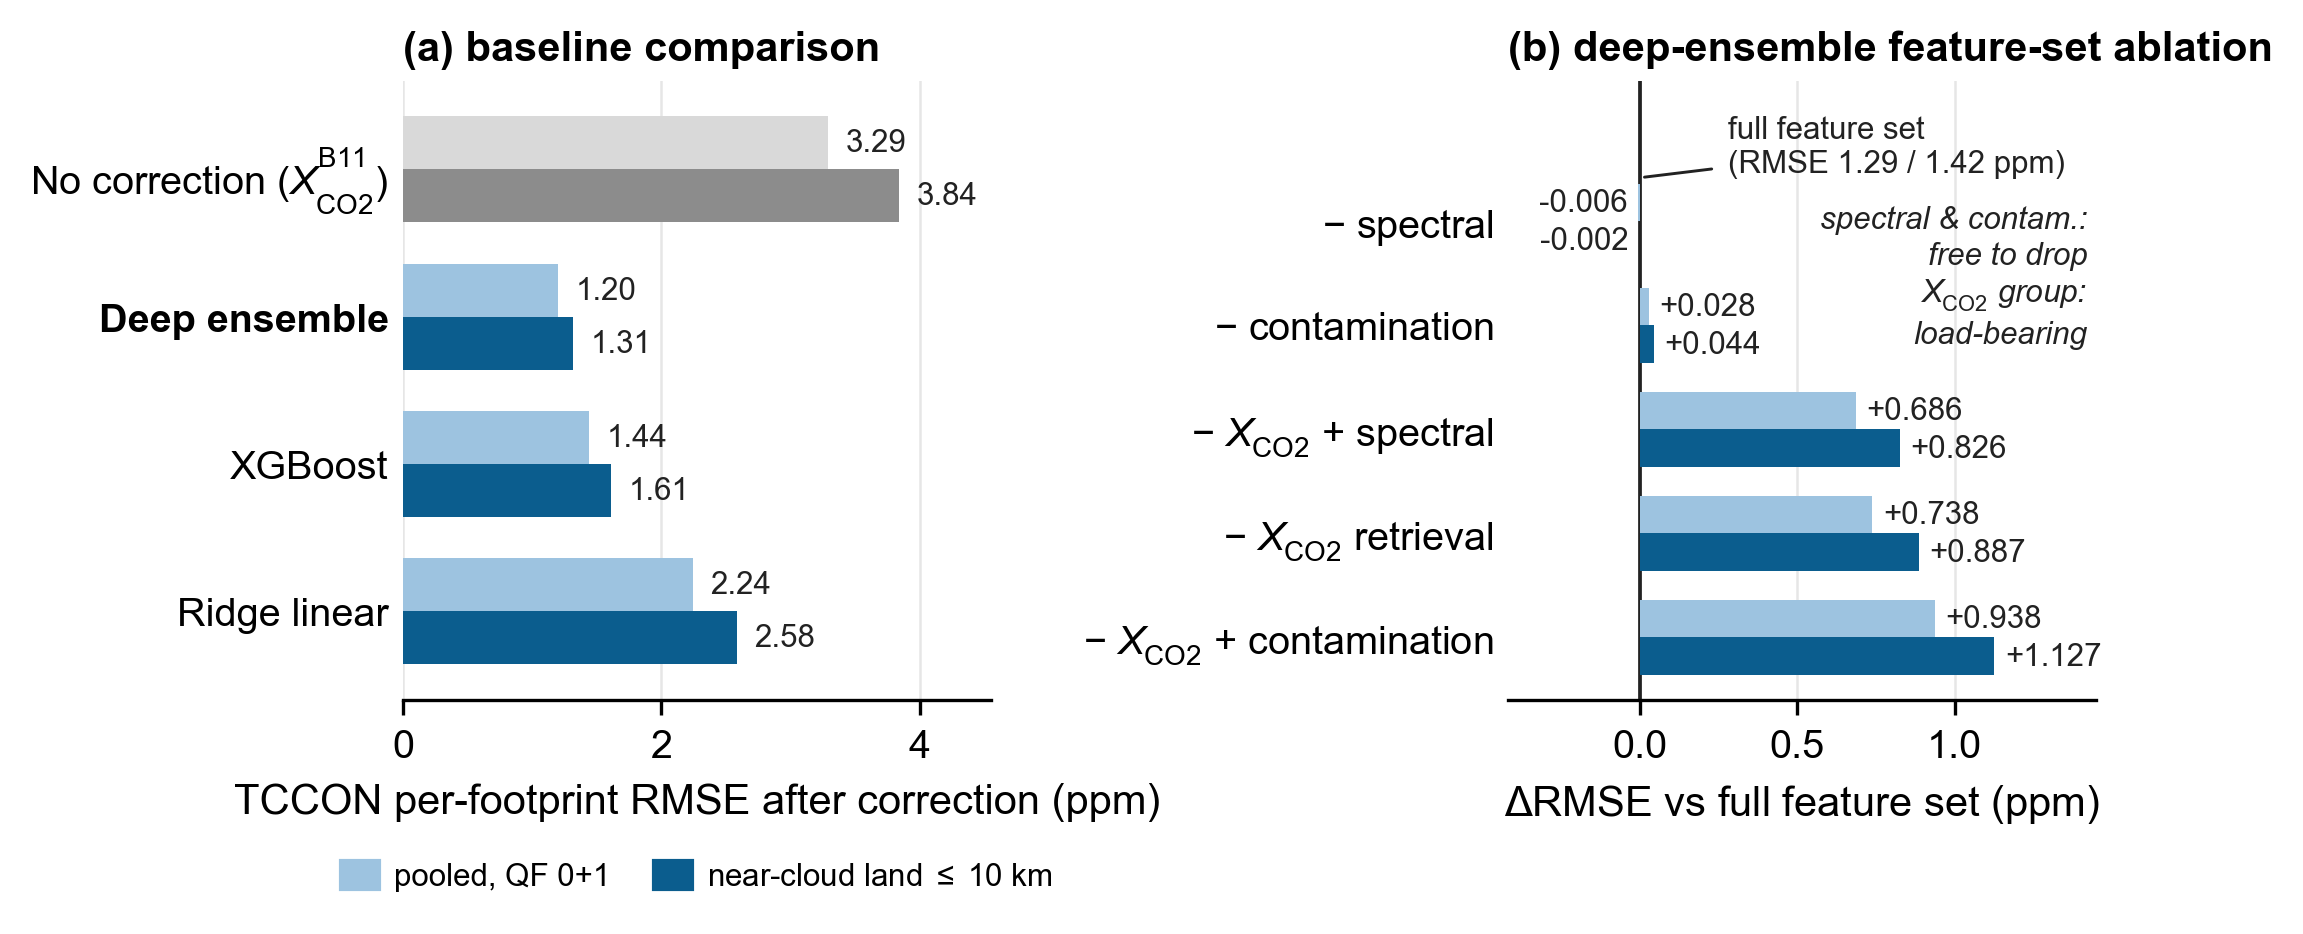
\includegraphics[width=0.8\textwidth]{figures/fig06_baseline_ablation.png}
\caption{Model and feature-set comparison under one protocol (identical features, date-blocked folds, and TCCON chain; AK-harmonised, r = 100 km / ±60 min). (a) TCCON per-footprint RMSE after correction, pooled over all quality flags (light, n = 105,683) and for the near-cloud land subset (≤ 10 km, dark, n = 75,157); the uncorrected product is shown for reference. (b) Feature-group ablation of the deep ensemble: $\Delta$RMSE relative to the full feature set.}
\label{fig:model_baseline_ablation}
\end{figure}



We then evaluate the permutation importance of each variable in the predictors by randomly shuffling each variable to see the increase in $\Delta \mathrm{RMSE}$ for the \emph{DE} model. Same as the results in Fig.~\ref{fig:model_baseline_ablation}b, the "\xcoraw − \xcoprior" plays the most essential role in the bias prediction for both the ocean and land models. The "$\Delta \mathrm{P}$/$\mathrm{P_{surface}^{prior}}$" shows as the second most important variable for both surfaces. Among the spectral path-length features, "var($l'$) of W\ce{CO2}" has the strongest response for the ocean model and the second strongest for the land model. The "$\exp$(\ce{O2}A intercept)" is the most important spectral path-length feature for the land model. The PC1 and PC2 of \ce{CO2} profile EOFs are also crucial for the prediction. Since cloud-bias information can be distributed across several variables in different ways, permuting individual variables may not capture the true importance of each feature. However, this analysis still helps us understand the potential importance of the features.




\begin{figure}[t]
\centering
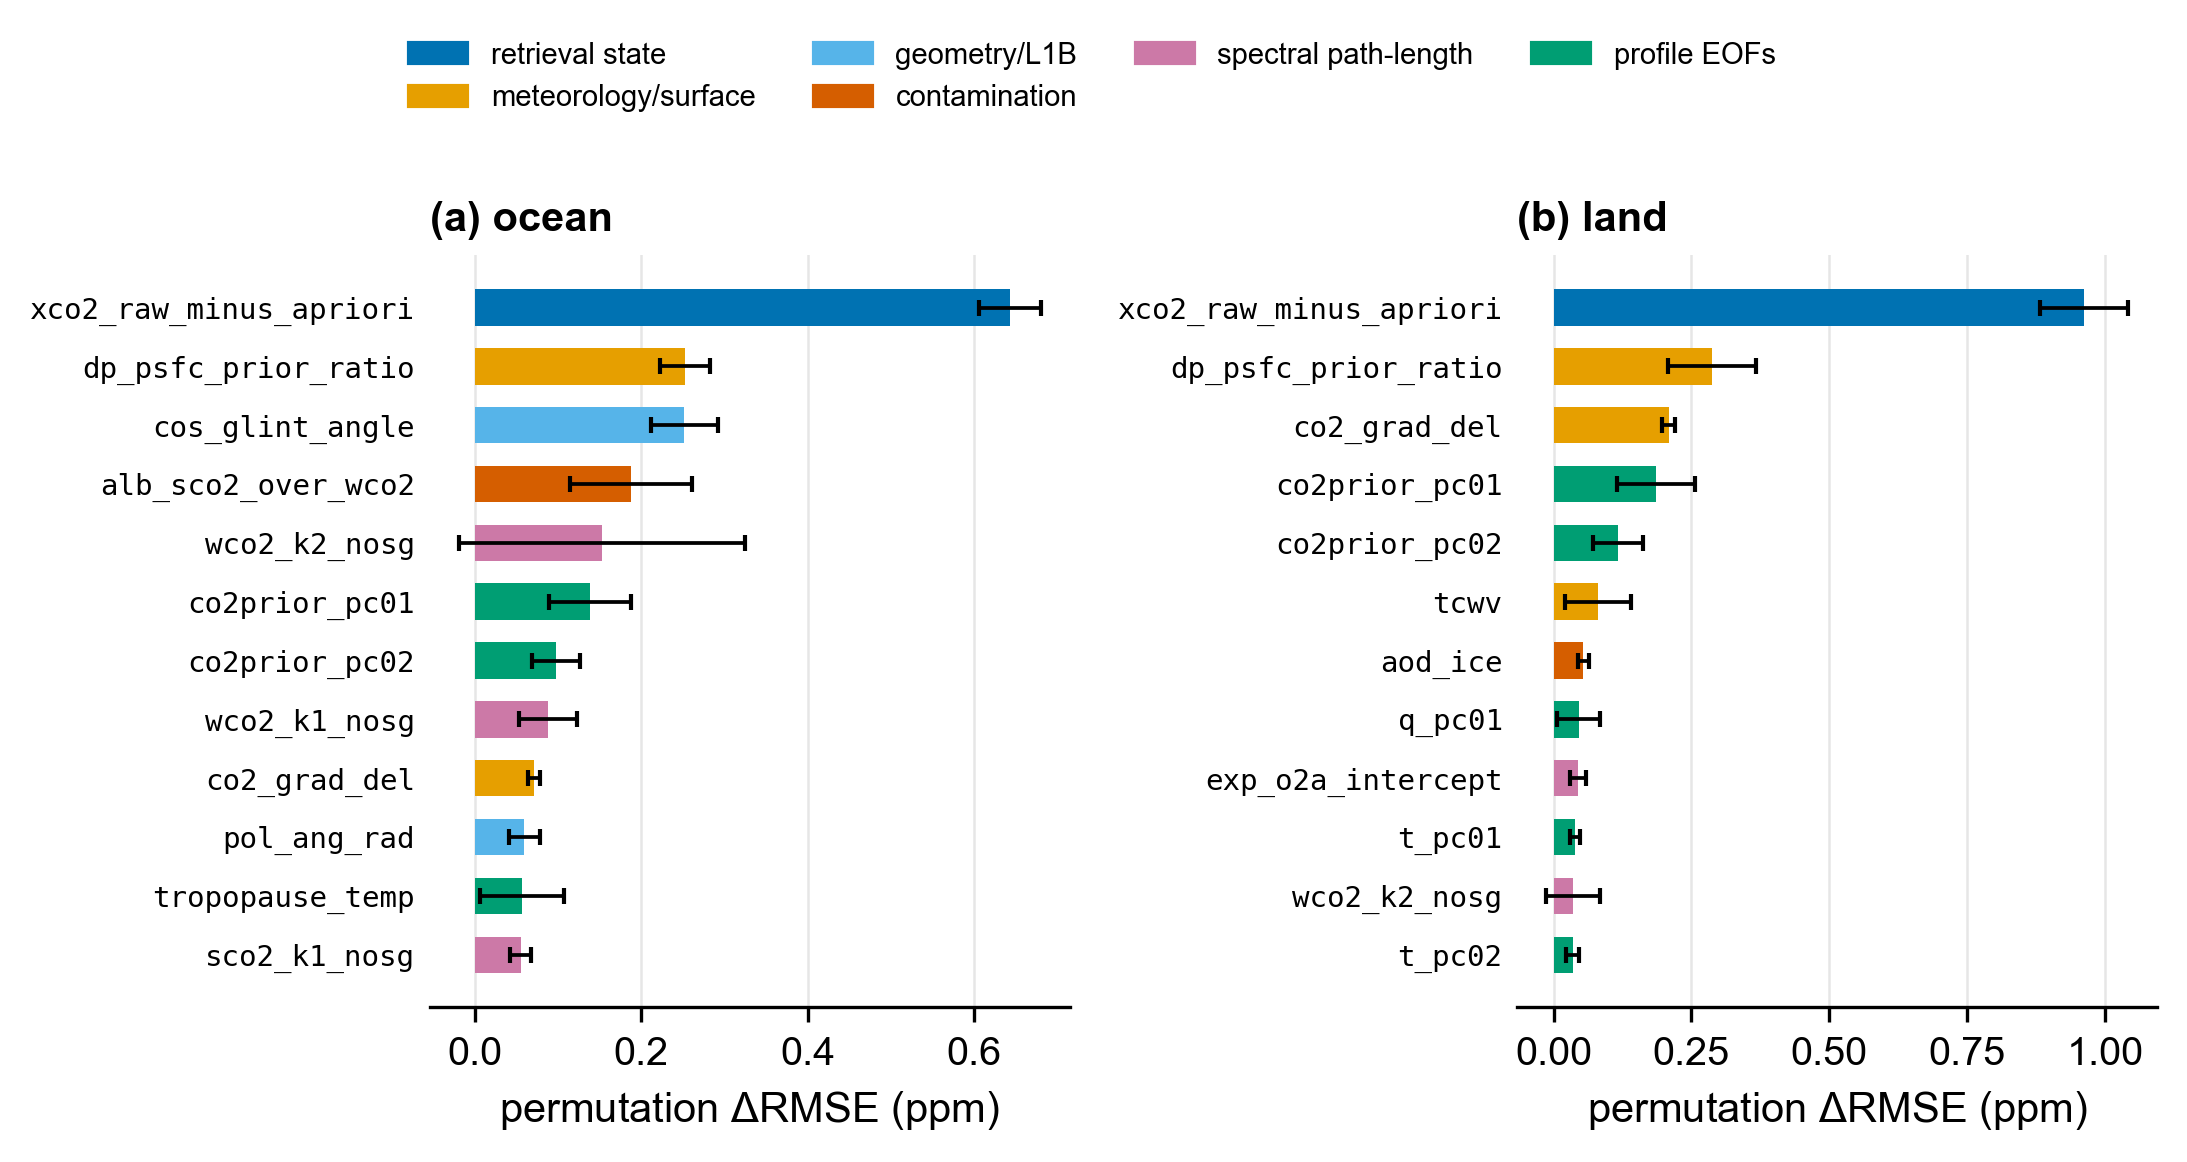
\includegraphics[width=0.8\textwidth]{figures/fig07_feature_importance.png}
\caption{Per-feature permutation importance of the production deep ensemble: increase in held-out fold RMSE when one feature is permuted (median over the five date-blocked folds; whiskers, fold standard deviation), for the twelve highest-ranked features over (a) ocean and (b) land. Bar color gives the predictor group of each feature, with feature definitions in Table~\ref{tab:predictor-inventory}. Groups are permuted jointly in the group-level attribution (Fig.~\ref{fig:model_baseline_ablation}b), which is the appropriate quantity under feature collinearity.}
\label{fig:DE_feature_importance}
\end{figure}




% Generated by manuscript/scripts/make_manuscript_tables.py — do not hand-edit.
% Requires booktabs. Define in the preamble:
%   \newcommand{\xcobc}{$X_{\mathrm{CO2}}^{\mathrm{bc}}$}
%   \newcommand{\xcoraw}{$X_{\mathrm{CO2}}^{\mathrm{raw}}$}
\begin{table}[htbp]
\centering
\caption{Footprint RMSE against AK-harmonized TCCON (ppm; 100\,km / $\pm$60\,min, 75 station-days) before (\xcobc) and after correction by the deep ensemble (DE), XGBoost (XGB), and ridge regression (Ridge). All models share the same footprints and before-column; the best corrected value per slice is in bold. QF is the operational \texttt{xco2\_quality\_flag}; cloud-distance slices split each surface at its production target radius (ocean 5\,km, land 15\,km; Sect.~3.1) and use the pre-drift cases where the Aqua-MODIS collocation is reliable.}
\label{tab:model-comparison}
\small
\begin{tabular}{lrrrrr}
\specialrule{1.2pt}{0pt}{2pt}
Slice & $n$ & Before & DE & XGB & Ridge \\
\midrule
Pooled, QF 0+1 & 105\,683 & 3.29 & \textbf{1.22} & 1.43 & 2.27 \\
Pooled, QF$\,$=$\,$0 & 56\,085 & 1.01 & \textbf{0.83} & 0.87 & 0.92 \\
Pooled, QF$\,$=$\,$1 & 49\,598 & 4.68 & \textbf{1.54} & 1.88 & 3.16 \\
Ocean & 6\,249 & 1.27 & \textbf{0.98} & 1.11 & 1.16 \\
Ocean, QF$\,$=$\,$1 & 1\,578 & 1.76 & \textbf{1.25} & 1.47 & 1.56 \\
Ocean $\leq$5\,km & 2\,645 & 1.54 & \textbf{1.12} & 1.24 & 1.26 \\
Ocean $\leq$5\,km, QF$\,$=$\,$1 & 1\,080 & 1.92 & \textbf{1.29} & 1.46 & 1.52 \\
Ocean $\geq$5\,km & 3\,604 & 1.02 & \textbf{0.86} & 1.01 & 1.08 \\
Land & 99\,434 & 3.38 & \textbf{1.23} & 1.45 & 2.32 \\
Land, QF$\,$=$\,$1 & 48\,020 & 4.75 & \textbf{1.55} & 1.89 & 3.20 \\
Land $\leq$15\,km & 81\,347 & 3.71 & \textbf{1.31} & 1.56 & 2.52 \\
Land $\leq$15\,km, QF$\,$=$\,$1 & 44\,107 & 4.94 & \textbf{1.59} & 1.94 & 3.32 \\
Land $\geq$15\,km & 18\,087 & 0.95 & \textbf{0.79} & 0.85 & 0.98 \\
\specialrule{1.2pt}{2pt}{0pt}
\end{tabular}
\end{table}






% Generated by manuscript/scripts/make_manuscript_tables.py — do not hand-edit.
% Requires booktabs. Define in the preamble:
%   \newcommand{\xcobc}{$X_{\mathrm{CO2}}^{\mathrm{bc}}$}
%   \newcommand{\xcoraw}{$X_{\mathrm{CO2}}^{\mathrm{raw}}$}
\begin{table}[htbp]
\centering
\caption{Feature-group ablation of the mix deep ensemble on TCCON (fp-RMSE, ppm; AK-harmonized reference, 100\,km / $\pm$60\,min). Each variant is retrained from scratch with one feature group removed, using the identical architecture, regularization, and date-blocked folds as the production model (full); all columns share the same footprints and before-column. Dropping the spectral-cumulant or aerosol-contamination groups is TCCON-neutral; the \xcoraw$-$prior departure block carries the correction.}
\label{tab:featureset-ablation}
\small
\begin{tabular}{lrrrrrrr}
\specialrule{1.2pt}{0pt}{2pt}
Slice & Before & full & $-$spec & $-$contam & $-$xco2 & $-$xco2$-$spec & $-$xco2$-$contam \\
\midrule
Pooled, QF 0+1 & 3.29 & \textbf{1.22} & 1.24 & 1.24 & 2.01 & 2.15 & 2.11 \\
Pooled, QF$\,$=$\,$0 & 1.01 & 0.83 & \textbf{0.83} & 0.85 & 1.03 & 0.99 & 1.12 \\
Pooled, QF$\,$=$\,$1 & 4.68 & \textbf{1.54} & 1.58 & 1.58 & 2.72 & 2.96 & 2.84 \\
Ocean & 1.27 & \textbf{0.98} & 1.00 & 0.99 & 1.13 & 1.15 & 1.15 \\
Land & 3.38 & \textbf{1.23} & 1.25 & 1.26 & 2.05 & 2.20 & 2.16 \\
Land, QF$\,$=$\,$1 & 4.75 & \textbf{1.55} & 1.59 & 1.59 & 2.76 & 2.99 & 2.88 \\
Land $\leq$10\,km & 3.84 & \textbf{1.33} & 1.36 & 1.36 & 2.30 & 2.47 & 2.42 \\
Land $\leq$10\,km, QF$\,$=$\,$1 & 5.00 & \textbf{1.60} & 1.64 & 1.63 & 2.88 & 3.14 & 3.01 \\
Land $\geq$10\,km & 1.00 & 0.84 & \textbf{0.83} & 0.90 & 0.91 & 0.97 & 0.98 \\
\specialrule{1.2pt}{2pt}{0pt}
\end{tabular}
\end{table}






\FloatBarrier

\subsection{Independent TCCON validation}
\label{sec:result-tccon_val}


%Use AK-harmonized TCCON as the primary reference and direct TCCON as a
%documented secondary comparison. Report the current production values only
%after regenerating the manuscript table from the frozen tag.

%The paragraph order should be:

1. one-sentence recap of the sample and coincidence criteria, citing
   Sect. 3.5;
2. mean absolute bias and footprint RMSE;
3. number of improved station-days;
4. Wilcoxon and site-clustered bootstrap results;
5. radius/window and QF0/QF1 sensitivity;
6. high-latitude and worsening cases.

Keep direct-reference results nearby but do not let the dual-reference
explanation obscure the AK-harmonized primary result.


After understanding the general performance of the \emph{DE} model in Sect.~\ref{sec:result-model_comp}, we then evaluate its correction capability compared to TCCON observations in detail. Again, all TCCON \xco are corrected following the description in Sect.~\ref{sec:method-eval-obs-xco2} to consider the difference in averaging kernels and prior profiles. The collocation search radius between the TCCON stations and the OCO-2 soundings is set to $100$~km, and the temporal search window to $\pm1$~h around the OCO-2 overpass. Note that these 75 station-days for 18 sites from December 2014 to December 2021 are chosen manually, as we want to have more available data for stations near the coastline, and we are unable to run all OCO-2 overpass cases.


Across all 75 station-days, the station-day mean absolute bias ($|$bias$|$) falls from 1.26$\pm$1.33 to 0.82$\pm$0.60 ppm and the per-footprint RMSE from 2.67 to 1.20 ppm (Fig.~\ref{fig:tccon_dumbbel}). The per-footprint RMSE improves in 71 of the 75 station-days, while the station-day mean bias improves in 46 of 75. The remaining 29 worsen only slightly, median $+0.28$ ppm, mostly from near-zero starting biases. The improvement is significant under a paired Wilcoxon test on station-day $|$bias$|$ (p = 0.0063, n = 75) and under site-clustered bootstrap intervals, with and without the high-latitude TCCON station Ny-Ålesund at 78.93$^\circ$N (Fig.~\ref{fig:tccon_significance_robustness}). The improvement holds at every collocation radius $\times$ window combination (25/50/100 km $\times$ $\pm$30/60/120 min), and it is largest at a tighter 50 km $\times$ $\pm$30 min window. This is expected, given that the correction is a spatially localized process. However, we use a larger search window to obtain more statistics and follow the $\pm1$~h window as in \citet{das2025oco2_v111_tccon_ggg2020}.

Additionally, we analyze QF=0 and QF=1 footprints separately (Fig.~\ref{app-fig:qf01_DE_eval}) and see that the $|$bias$|$ significantly decreases for QF=1 from 1.57$\pm$1.43 to 0.89$\pm$0.62, with the footprint RMSE reduced from 3.19 to 1.31. The $|$bias$|$ and footprint RMSE also improve for QF=0 but with smaller magnitudes. This is expected, as footprints with QF=0 have better retrieval quality and could be less influenced by clouds. We also see that the correction is larger when the station-mean nearest-cloud distance of OCO-2 footprints is small, confirming that our correction works in the right direction.

For all TCCON stations we used, Ny-Ålesund is the only station in our comparison poleward of 60$^\circ$ latitude, and high-latitude scenes are correspondingly rare in the training population. Only 5.3\,\% of the 17.8 million training
footprints lie poleward of $|60^\circ|$ (936,178) and 2.3 \% poleward of $|70^\circ|$ (411,649). Nevertheless, the ten Ny-Ålesund station-days receive the strongest corrections in the network. The station-day mean $|$bias$|$ falls from 2.18 to 1.31~ppm and the per-footprint RMSE from 4.74 to 1.95~ppm, both roughly twice the network-average improvement. The largest single correction of the comparison (from $-8.20$ to $-0.86$~ppm on 17 June 2017) occurs here. This is also why excluding
Ny-Ålesund reduces the magnitude of all three aggregate improvements in Fig.~\ref{fig:tccon_significance_robustness}a while their significance is retained ($p \le 0.016$). The headline result is not driven by this single site, but the site benefits from the correction more than any
other. At the same time, the corrected Ny-Ålesund residuals remain the largest in the network and are sign-consistent (positive in 7 of 10 station-days, up to $+2.9$~ppm), so a systematic high-latitude bias
survives the correction. We attribute this remaining bias to the thin training support poleward of 60$^\circ$ together with the extreme observation geometry (high solar zenith angle, seasonal snow and ice), and we regard the high-latitude regime as the part of the domain where the correction is least constrained. Additional high-latitude references (e.g., Sodankylä, East Trout Lake, Eureka) would be needed to validate it independently, and we return to this limit in Sect.~\ref{sec:limitation}.


The worsening cases are informative about the limits of the anomaly formulation rather than about the model fit. The bright-surface stratum (\ce{O2}A-band albedo $> 0.4$; 12{,}037 footprints, 11.4\,\% of the TCCON comparison set) shows the largest post-correction residual (1.55~ppm) and a worsened-footprint fraction of 0.50. This is not a prediction failure: on genuinely held-out dates in cross-validation, the model's anomaly skill is independent of albedo (residual RMSE 0.53--0.60~ppm and calibration $\langle z^2\rangle \approx 1.1$ across all albedo deciles), and even at TCCON the correction reduces the bright-surface footprint RMSE from 4.58 to 1.55~ppm. What remains after correction over bright scenes is a bias component that is nearly constant within an overpass. Such a common-mode component cancels in the within-orbit anomaly target by construction, so the model is never trained to remove it; the correction takes out the anomaly part and leaves the common-mode part behind. Because the remaining residual is then uncorrelated with the applied correction, the per-footprint worsened-or-improved count degenerates toward a coin flip (0.50, against 0.19--0.39 elsewhere), while the aggregate error still improves. The bright-surface stratum is therefore under-corrected rather than mis-corrected, in line with the high-AOD stratum, and both point to the same future extension: a complementary term for along-track common-mode bias, which the present per-footprint anomaly correction intentionally does not model.





\begin{figure}[t]
\centering
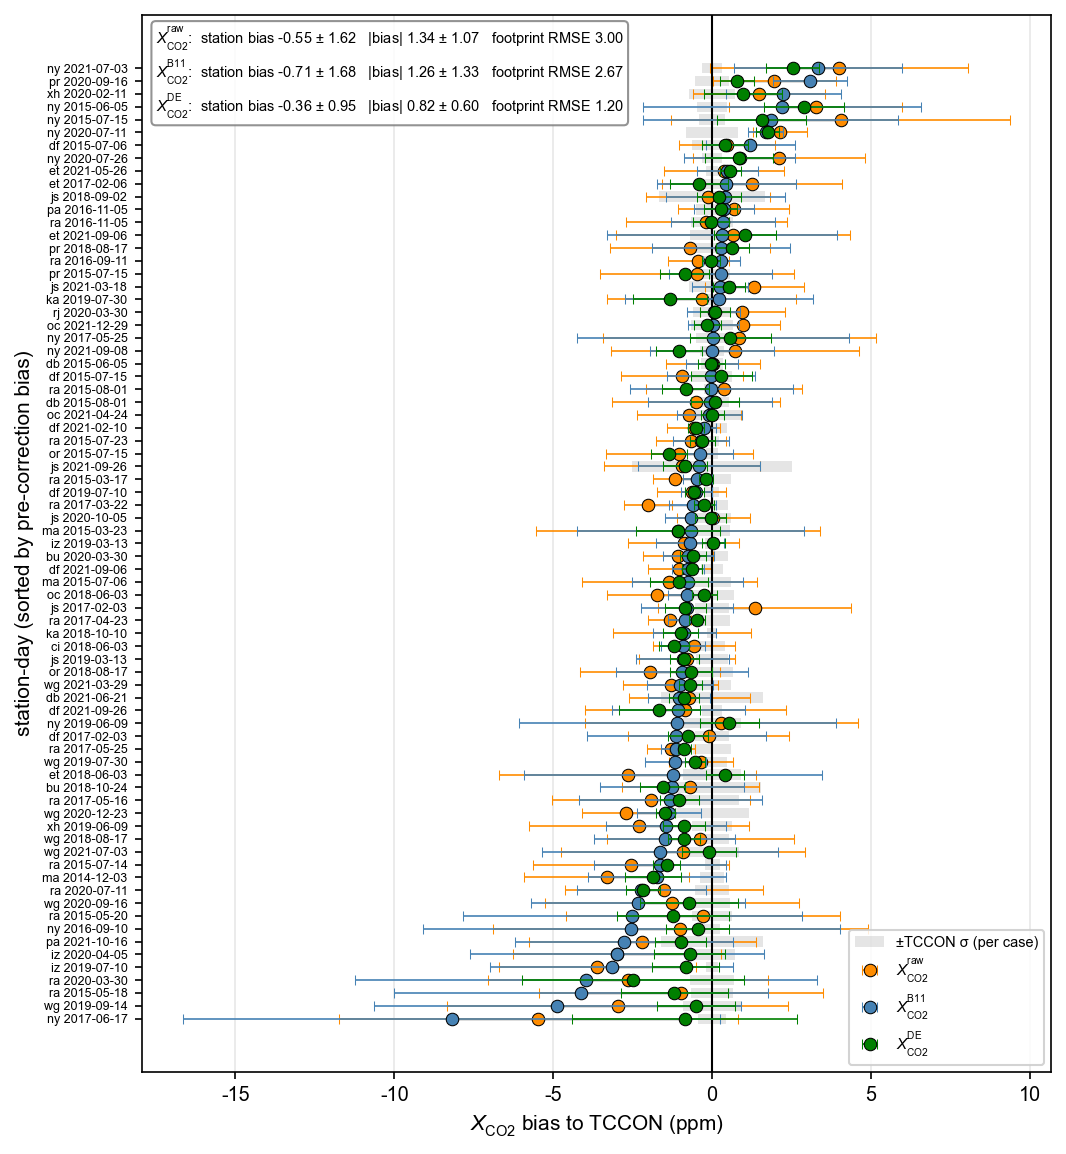
\includegraphics[width=0.8\textwidth]{figures/fig08_tccon_dumbbell.png}
\caption{Independent TCCON validation (AK-harmonised reference; before-vs-after differences are invariant to it): station-day mean bias before and after correction for all 75 station-days (18 sites, 2014–2021; r = 100 km, ±60 min).}
\label{fig:tccon_dumbbel}
\end{figure}



\begin{figure}[t]
\centering
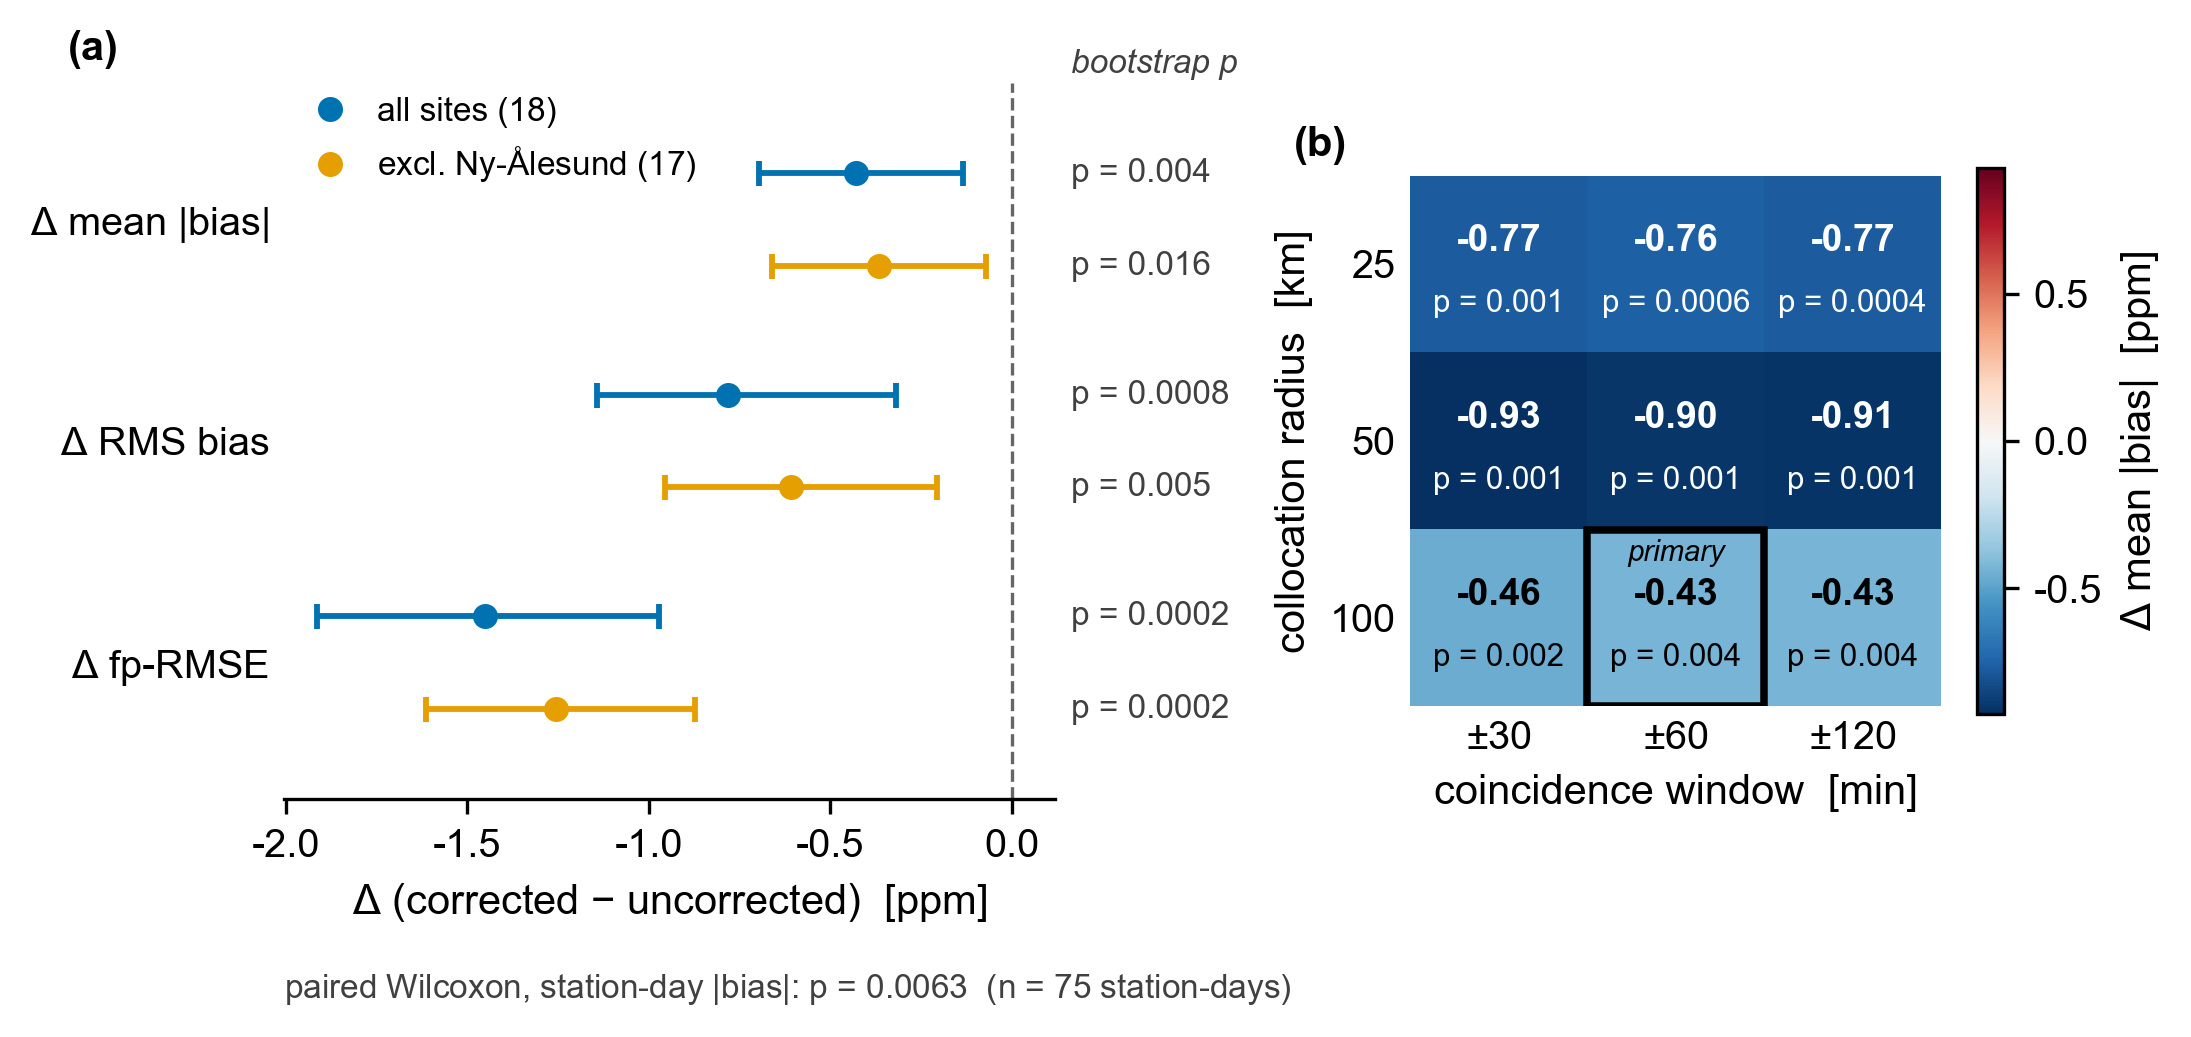
\includegraphics[width=0.8\textwidth]{figures/fig09_significance_robustness.png}
\caption{Significance and robustness of the TCCON validation: site-clustered bootstrap estimates with 95 \% confidence intervals for the change in station-day mean $|$bias$|$, RMS bias, and per-footprint RMSE (all sites and excluding Ny-Ålesund), and the change in mean $|$bias$|$ across collocation radius (25/50/100 km) × window (±30/60/120 min).}
\label{fig:tccon_significance_robustness}
\end{figure}





%% Generated by manuscript/scripts/make_manuscript_tables.py — do not hand-edit.
% Requires booktabs. Define in the preamble:
%   \newcommand{\xcobc}{$X_{\mathrm{CO2}}^{\mathrm{bc}}$}
%   \newcommand{\xcoraw}{$X_{\mathrm{CO2}}^{\mathrm{raw}}$}
\begin{table}[htbp]
\centering
\caption{Station-equal mean absolute bias to AK-harmonized TCCON (ppm): each station's footprint-weighted mean bias is taken in absolute value and averaged with equal station weights (18 stations). Best corrected value per row in bold.}
\label{tab:station-equal-bias}
\small
\begin{tabular}{lrrrr}
\specialrule{1.2pt}{0pt}{2pt}
QF & Before & DE & XGB & Ridge \\
\midrule
QF 0+1 & 0.98 & \textbf{0.73} & 0.74 & 0.83 \\
QF$\,$=$\,$0 & 0.60 & 0.60 & 0.63 & \textbf{0.58} \\
QF$\,$=$\,$1 & 1.36 & 0.82 & \textbf{0.80} & 0.96 \\
\specialrule{1.2pt}{2pt}{0pt}
\end{tabular}
\end{table}






\FloatBarrier

\subsection{Distinguishing correction from smoothing}
\label{sec:result-corr_smooth}


A possible objection to the decrease in footprint RMSE result of Sect.~\ref{sec:result-tccon_val} is that the \emph{DE} model may act as a local low-pass filter. Since the near-cloud bias appears as short-scale structure along the orbit, any procedure that averages neighboring footprints would also collapse the within-overpass scatter, and the station-day comparison might not distinguish the two. To test this possibility directly, we construct a feature-free smoother null and evaluate it with exactly the same footprints, output guards, and AK-harmonized TCCON chain as the production correction.

For footprint $i$, the smoothed product is the orbit-local running mean of the operational product,
%
\begin{equation}
  X^{\mathrm{sm}(W)}_{\mathrm{CO2},i}
  = \frac{1}{\left|\mathcal{N}_i(W)\right|}
    \sum_{j \in \mathcal{N}_i(W)} X^{\mathrm{B11}}_{\mathrm{CO2},j},
  \qquad
  \mathcal{N}_i(W)
  = \left\{\, j \;:\; \left|t_j - t_i\right| \le W \,\right\},
  \label{eq:smoother}
\end{equation}
%
where $t_i$ is the sounding time and $\mathcal{N}_i(W)$ is restricted to the same contiguous along-track segment (a time gap larger than 30~s starts a new segment) and the same surface type as footprint $i$, mirroring the per-surface construction of the model; the footprint itself is included in the mean, as for any symmetric smoother. The implied pseudo-correction is $\mu^{\mathrm{sm}}_i = X^{\mathrm{B11}}_{\mathrm{CO2},i} - X^{\mathrm{sm}(W)}_{\mathrm{CO2},i}$, which replaces the deep-ensemble $\mu_i$ in the evaluation chain. We test half-widths $W = 10$, 30, and 100~s, corresponding to roughly $\pm 67$, $\pm 200$, and $\pm 675$~km along track. The smoother uses no predictor features and no cloud information: it is the strongest form of the ``the correction only smooths'' hypothesis.

The two diagnostics separate cleanly (Fig.~\ref{fig:smoother_null}). On the within-overpass footprint scatter, the smoother is stronger than the \emph{DE} model as expected. The per-case mean scatter falls from 2.23~ppm to 0.66, 0.51, and 0.35~ppm for $W = 10$, 30, and 100~s, compared with 0.78~ppm for the deep ensemble. A running mean minimizes local variance by construction, so on this metric alone the null cannot be rejected. The station-day mean $|$bias$|$ to TCCON, however, is left essentially unmoved by the smoother: 1.26~ppm before correction against 1.24, 1.20, and 1.20~ppm after smoothing, whereas the deep ensemble reduces it to 0.82~ppm. The reason is structural: because the running mean approximately preserves the overpass-mean \xco, it can only redistribute the error among footprints, not remove it, while the deep ensemble shifts the mean itself. We conclude that variance removal alone cannot reproduce the observed bias reduction, and that the validation improvement of Sect.~4.4 reflects a genuine correction of the near-cloud bias rather than local denoising. Figure~\ref{fig:smoother_null} shows the $W = 30$~s arm; the $\pm 10$ and $\pm 100$~s arms behave the same way and are given in Appendix~\ref{app:null-test} (Fig.~\ref{app-fig:smoother_null_full}).




The smoother collapses footprint scatter more strongly than the \emph{DE} model (0.35–0.66 vs 0.78 ppm) yet leaves the TCCON station-day mean $|$bias$|$ essentially unmoved (1.20–1.24 ppm, against 0.82 ppm for the model). In other words, variance removal alone cannot produce the observed bias reduction, and the correction by the \emph{DE} model reduces both observed bias and spread.




\begin{figure}[t]
\centering
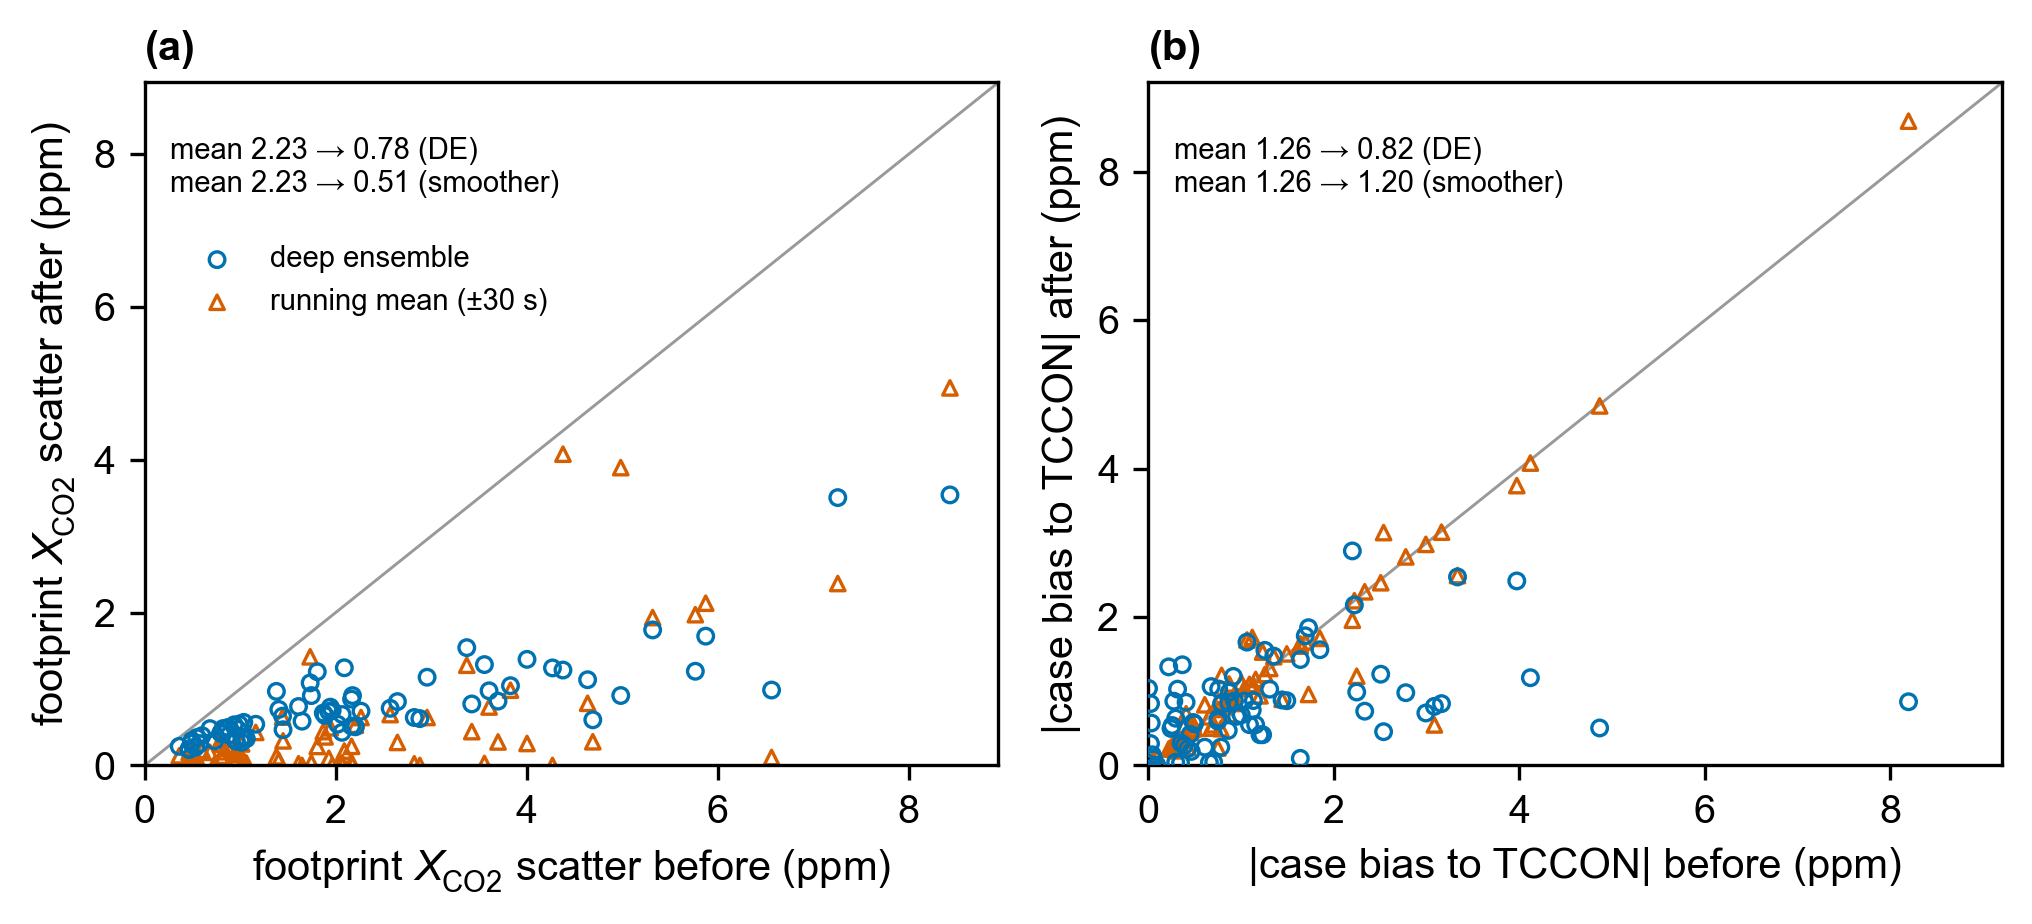
\includegraphics[width=0.8\textwidth]{figures/fig10_smoother_null.png}
\caption{Correction versus smoothing null test. A feature-free orbit-local running-mean smoother (±10/30/100 s half-widths, screened by the same input guards as the production correction) compared with the deep ensemble on footprint scatter (a) and TCCON station-day mean $|$bias$|$ (b).}
\label{fig:smoother_null}
\end{figure}



\FloatBarrier

\subsection{Ocean validation and far-cloud controls}
\label{sec:result-ocean_far_cldl}

Present ATom, shipborne EM27/SUN, and the far-cloud/clear-day cases where the
correction is nearly inert. Treat these as independent corroboration, not as
equivalent in statistical weight to TCCON. State the limited sample and
reference-scale caveats.


After we validate the correction of the \emph{DE} model in Sect.~\ref{sec:result-tccon_val,sec:result-corr_smooth}, we extend our validation to two different in-situ measurements to provide more validation tests over the ocean, considering that all TCCON stations are still over land and only part of them are close to the ocean coastline. We identify 17 ATom and OCO-2 co-located legs and 4 shipborne (MORE-2 and MR21-01) and OCO-2 co-located legs. We construct the pseudo-column \xcoatom from the in-situ airborne \xco measurement for comparison (Sect.~\ref{sec:method-eval-obs-xco2}), and use \xcoship directly as no prior profiles and averaging kernels are available.


Across the 17 ATom legs (14 near-cloud), the near-cloud improvement is a scatter reduction, not an offset shift. The median $|$residual$|$ ($|$\xcooco - \xcoatom$|$) falls from 0.53 to 0.45 ppm and the across-leg spread from ±0.72 to ±0.58 ppm, while the signed mean bias is essentially unchanged (+0.19 → +0.20 ppm, well within the per-leg pseudo-column $\sigma$ of 0.10–0.19 ppm). The far-cloud date (9 October 2017) is a negative control that the correction leaves nearly unchanged (Fig.~\ref{fig:ocean-validation}a, b). Against the shipborne EM27/SUN spectrometers (4 cases, 3 near-cloud), the correction collapses footprint scatter (mean $\sigma$ 0.63 → 0.27 ppm, against a mean ship reference $\sigma$ of 0.29 ppm) without moving the clear-sky control day (22 June 2019). The increase of $|$residual$|$ ($|$\xcooco - \xcoship$|$) absolute offset (all-case mean +0.99 ± 0.70 before, +1.18 ± 0.81 ppm after) could be dominated by reference-scale differences, considering no prior profiles and averaging kernel-harmonization applied  (Fig.~\ref{fig:ocean-validation}c, d). Note that we have limited temporal and spatial overpass samples compared to TCCON validations for ATom and Shipborne measurements comparison. The comparison with ATom in-situ and shipborne EM27/SUN measurements should be treated as independent corroboration, not as equivalent in statistical weight to TCCON.


Figure~\ref{app-fig:atom_far_cld,app-fig:ship_far_cld} illustrate little change in values and distribution for far-cloud footprints for ATom and Ship observation cases. These two negative controls are consistent with the far-cloud behavior in the TCCON comparison itself. In the station-day groups beyond the
production reference radii (ocean $\geq 5$~km, land $\geq 15$~km; Table~\ref{tab:model_comparison}), the pre-correction error is already small, and the correction leaves it slightly improved rather than degraded (footprint RMSE 1.02 $\rightarrow$ 0.86 and 0.95 $\rightarrow$ 0.79~ppm, respectively; see also the cloud-distance dependence in Fig.~\ref{app-fig:qf01_DE_eval}), so the near-inert far-cloud response over the ocean is not a small-sample artifact.



\begin{figure}[t]
\centering
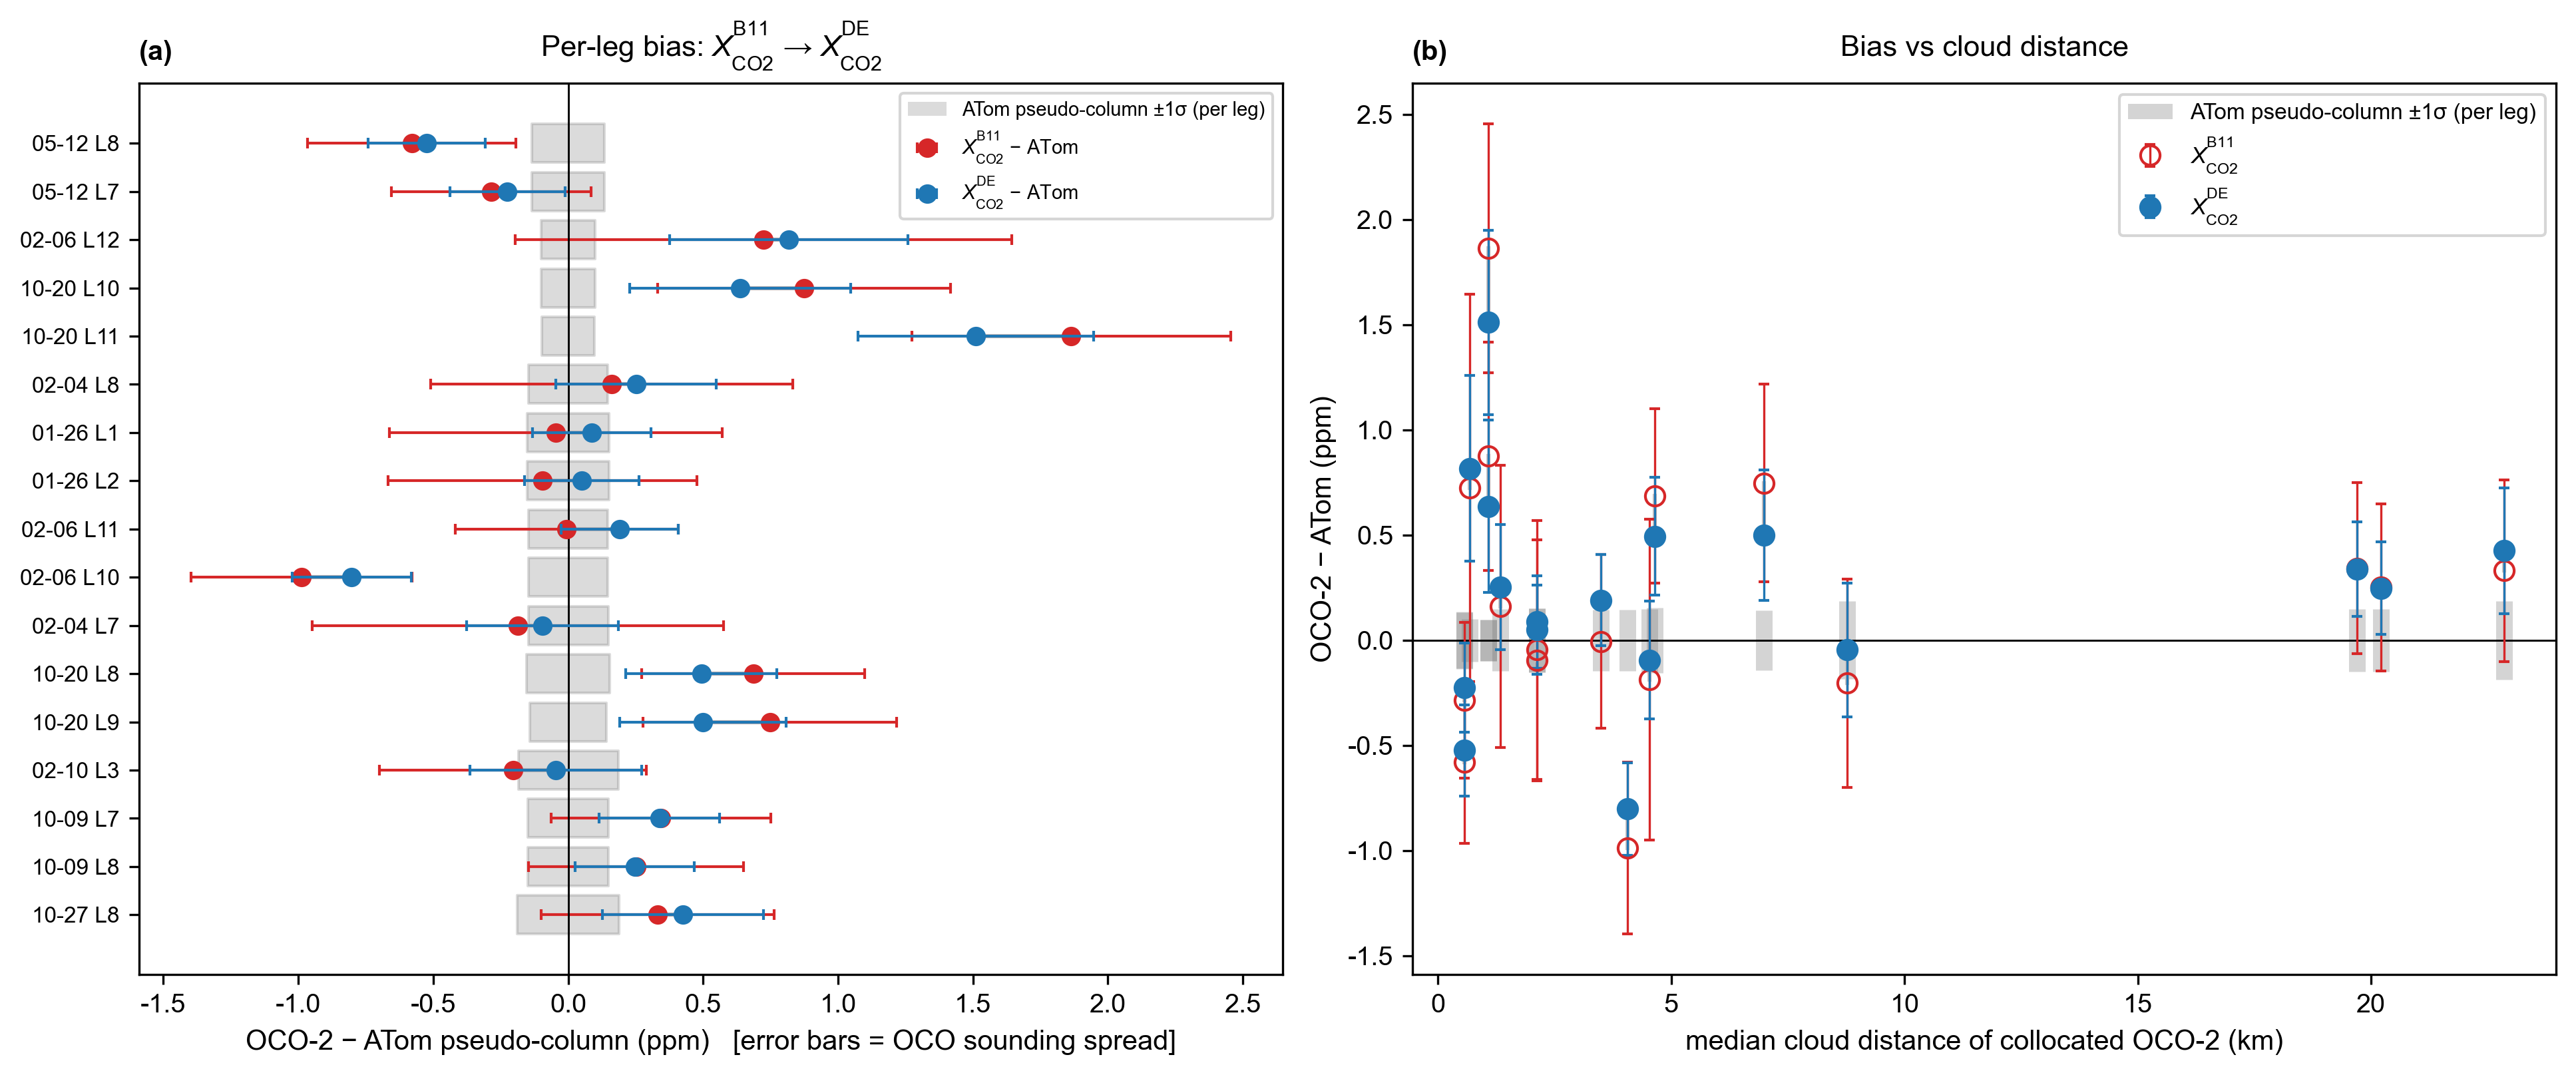
\includegraphics[width=0.95\textwidth]{figures/fig11a_atom_summary.png}\\[4pt]
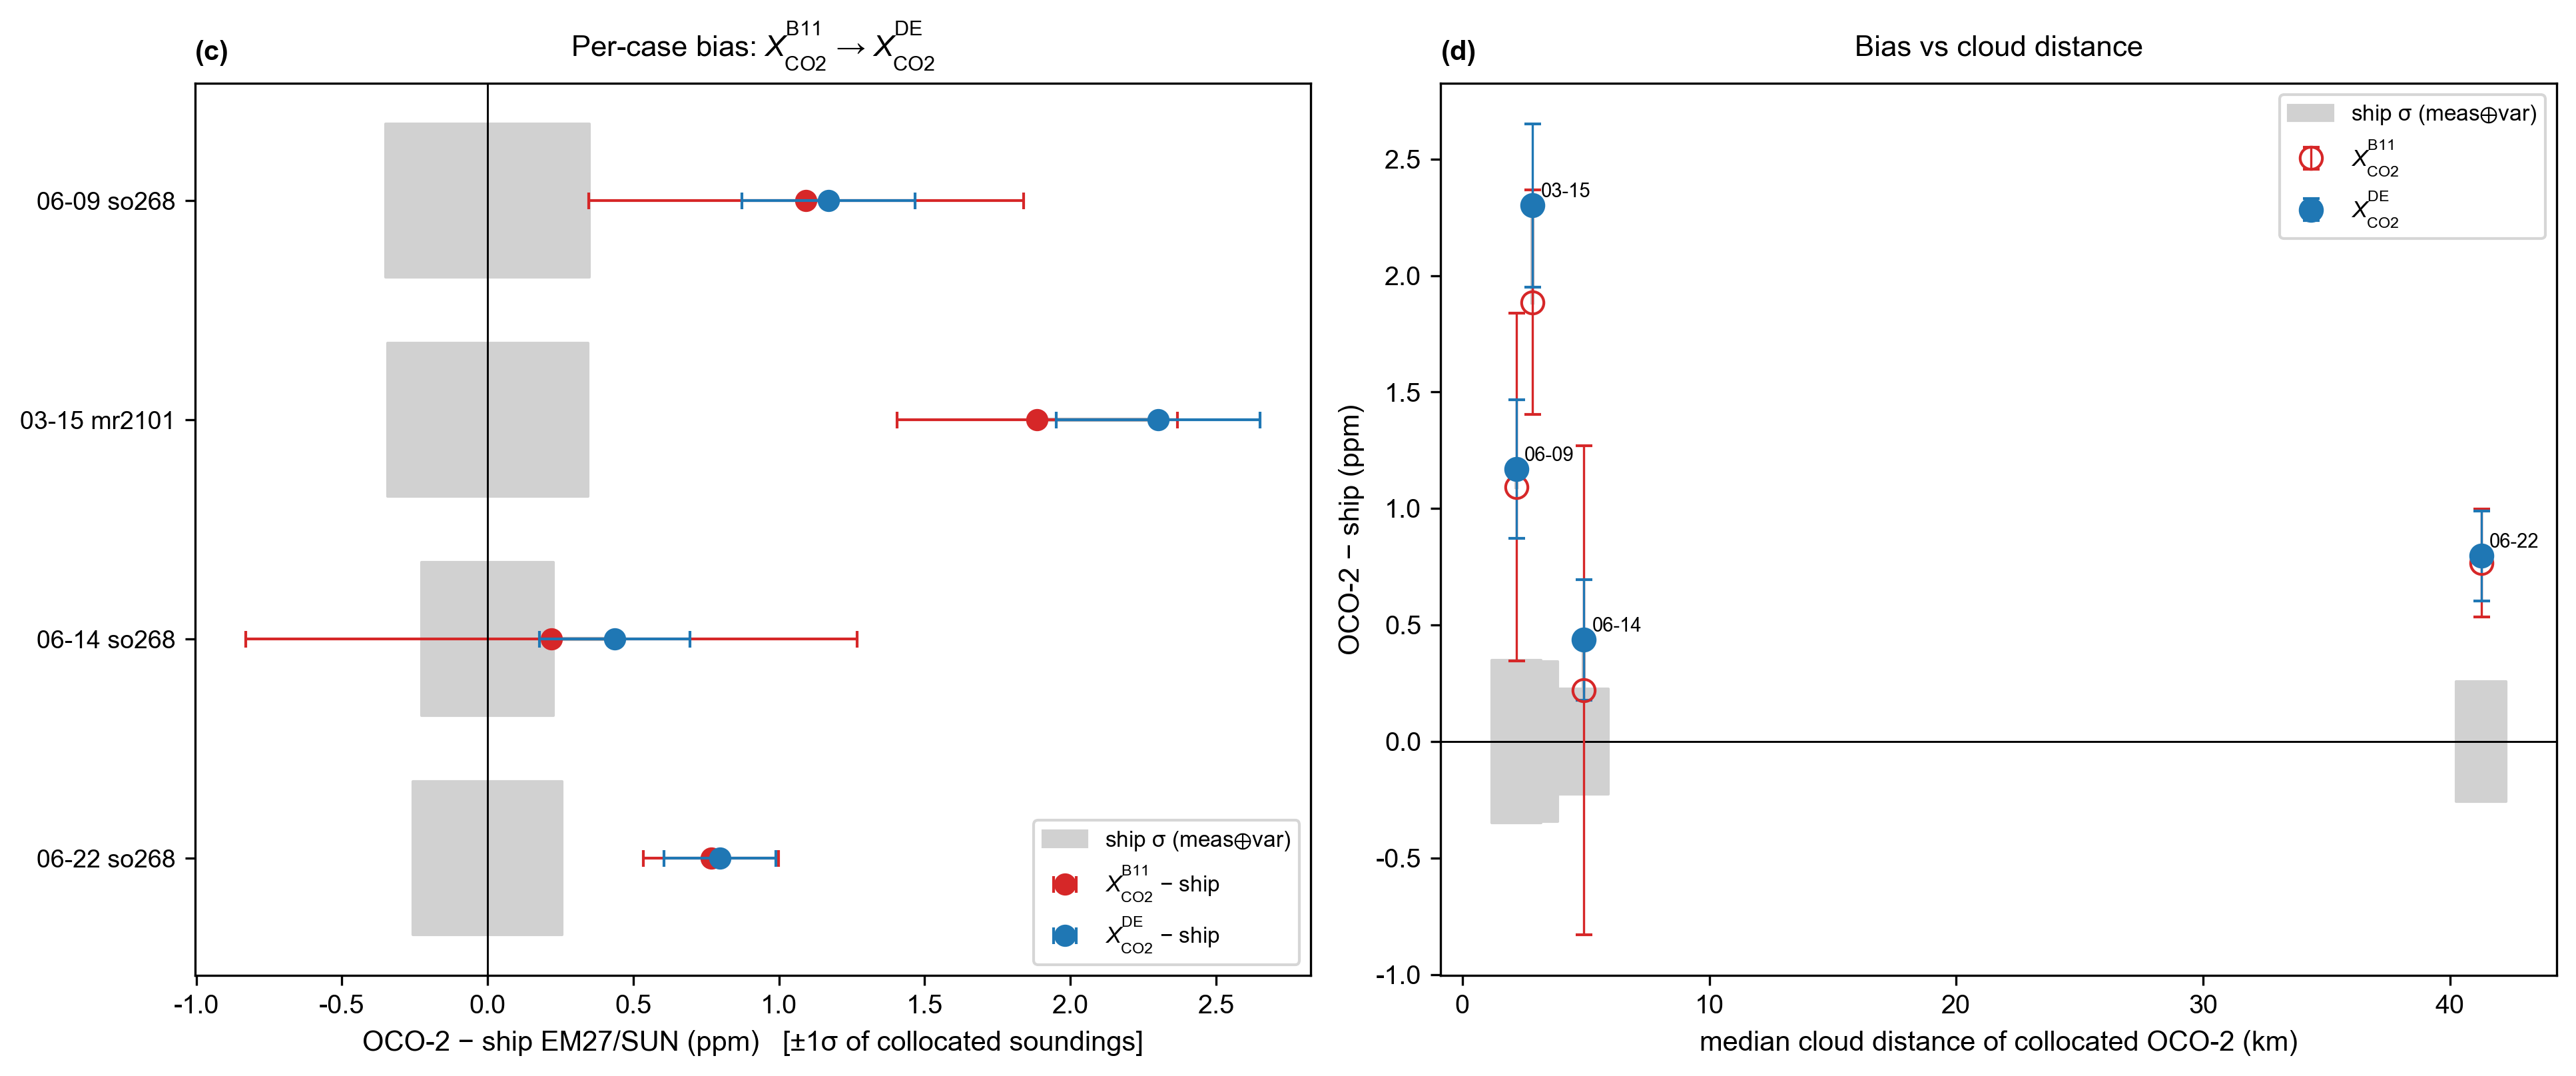
\includegraphics[width=0.95\textwidth]{figures/fig11b_ship_summary.png}
\caption{Independent ocean corroboration. (a, b) ATom aircraft pseudo-column comparison (8 dates, 17 collocated legs, AK-smoothed; the unmeasured stratosphere is filled with the OCO-2 prior so it cancels in the comparison), including the far-cloud negative-control date (9 October 2017): per-leg signed bias before and after correction, and the same residuals against median cloud distance; grey bands mark each leg's own pseudo-column ±1σ. (c, d) Shipborne EM27/SUN comparison (R/V Sonne MORE-2 and R/V Mirai MR21-01; 100 km / ±2 h), including the clear-sky control day (22 June 2019), in the same two views; grey bands mark the ship reference uncertainty (measurement ⊕ within-window variability).}
\label{fig:ocean-validation}
\end{figure}





\FloatBarrier

\subsection{Plume preservation and correction safety}
\label{sec:result-plume}


Local smoothing is primarily attributable to the retrieval-state channel, not to the photon path-length features.


The ~+0.6 ppm enhancement at closest approach to the Westar plant survives the correction essentially unchanged (Fig.~\ref{fig:plume-preservation}a). In the two flagged removal windows, the \ce{O2}A band shifts as strongly as the \ce{CO2} bands (Fig.~\ref{fig:plume-preservation}b) — the all-band fingerprint of cloud contamination rather than of a real plume, whose signature would be confined to the CO2 bands; the worst-case plume signal removable through the spectral channel is ≤ 0.21 ppm.




\begin{figure}[t]
\centering
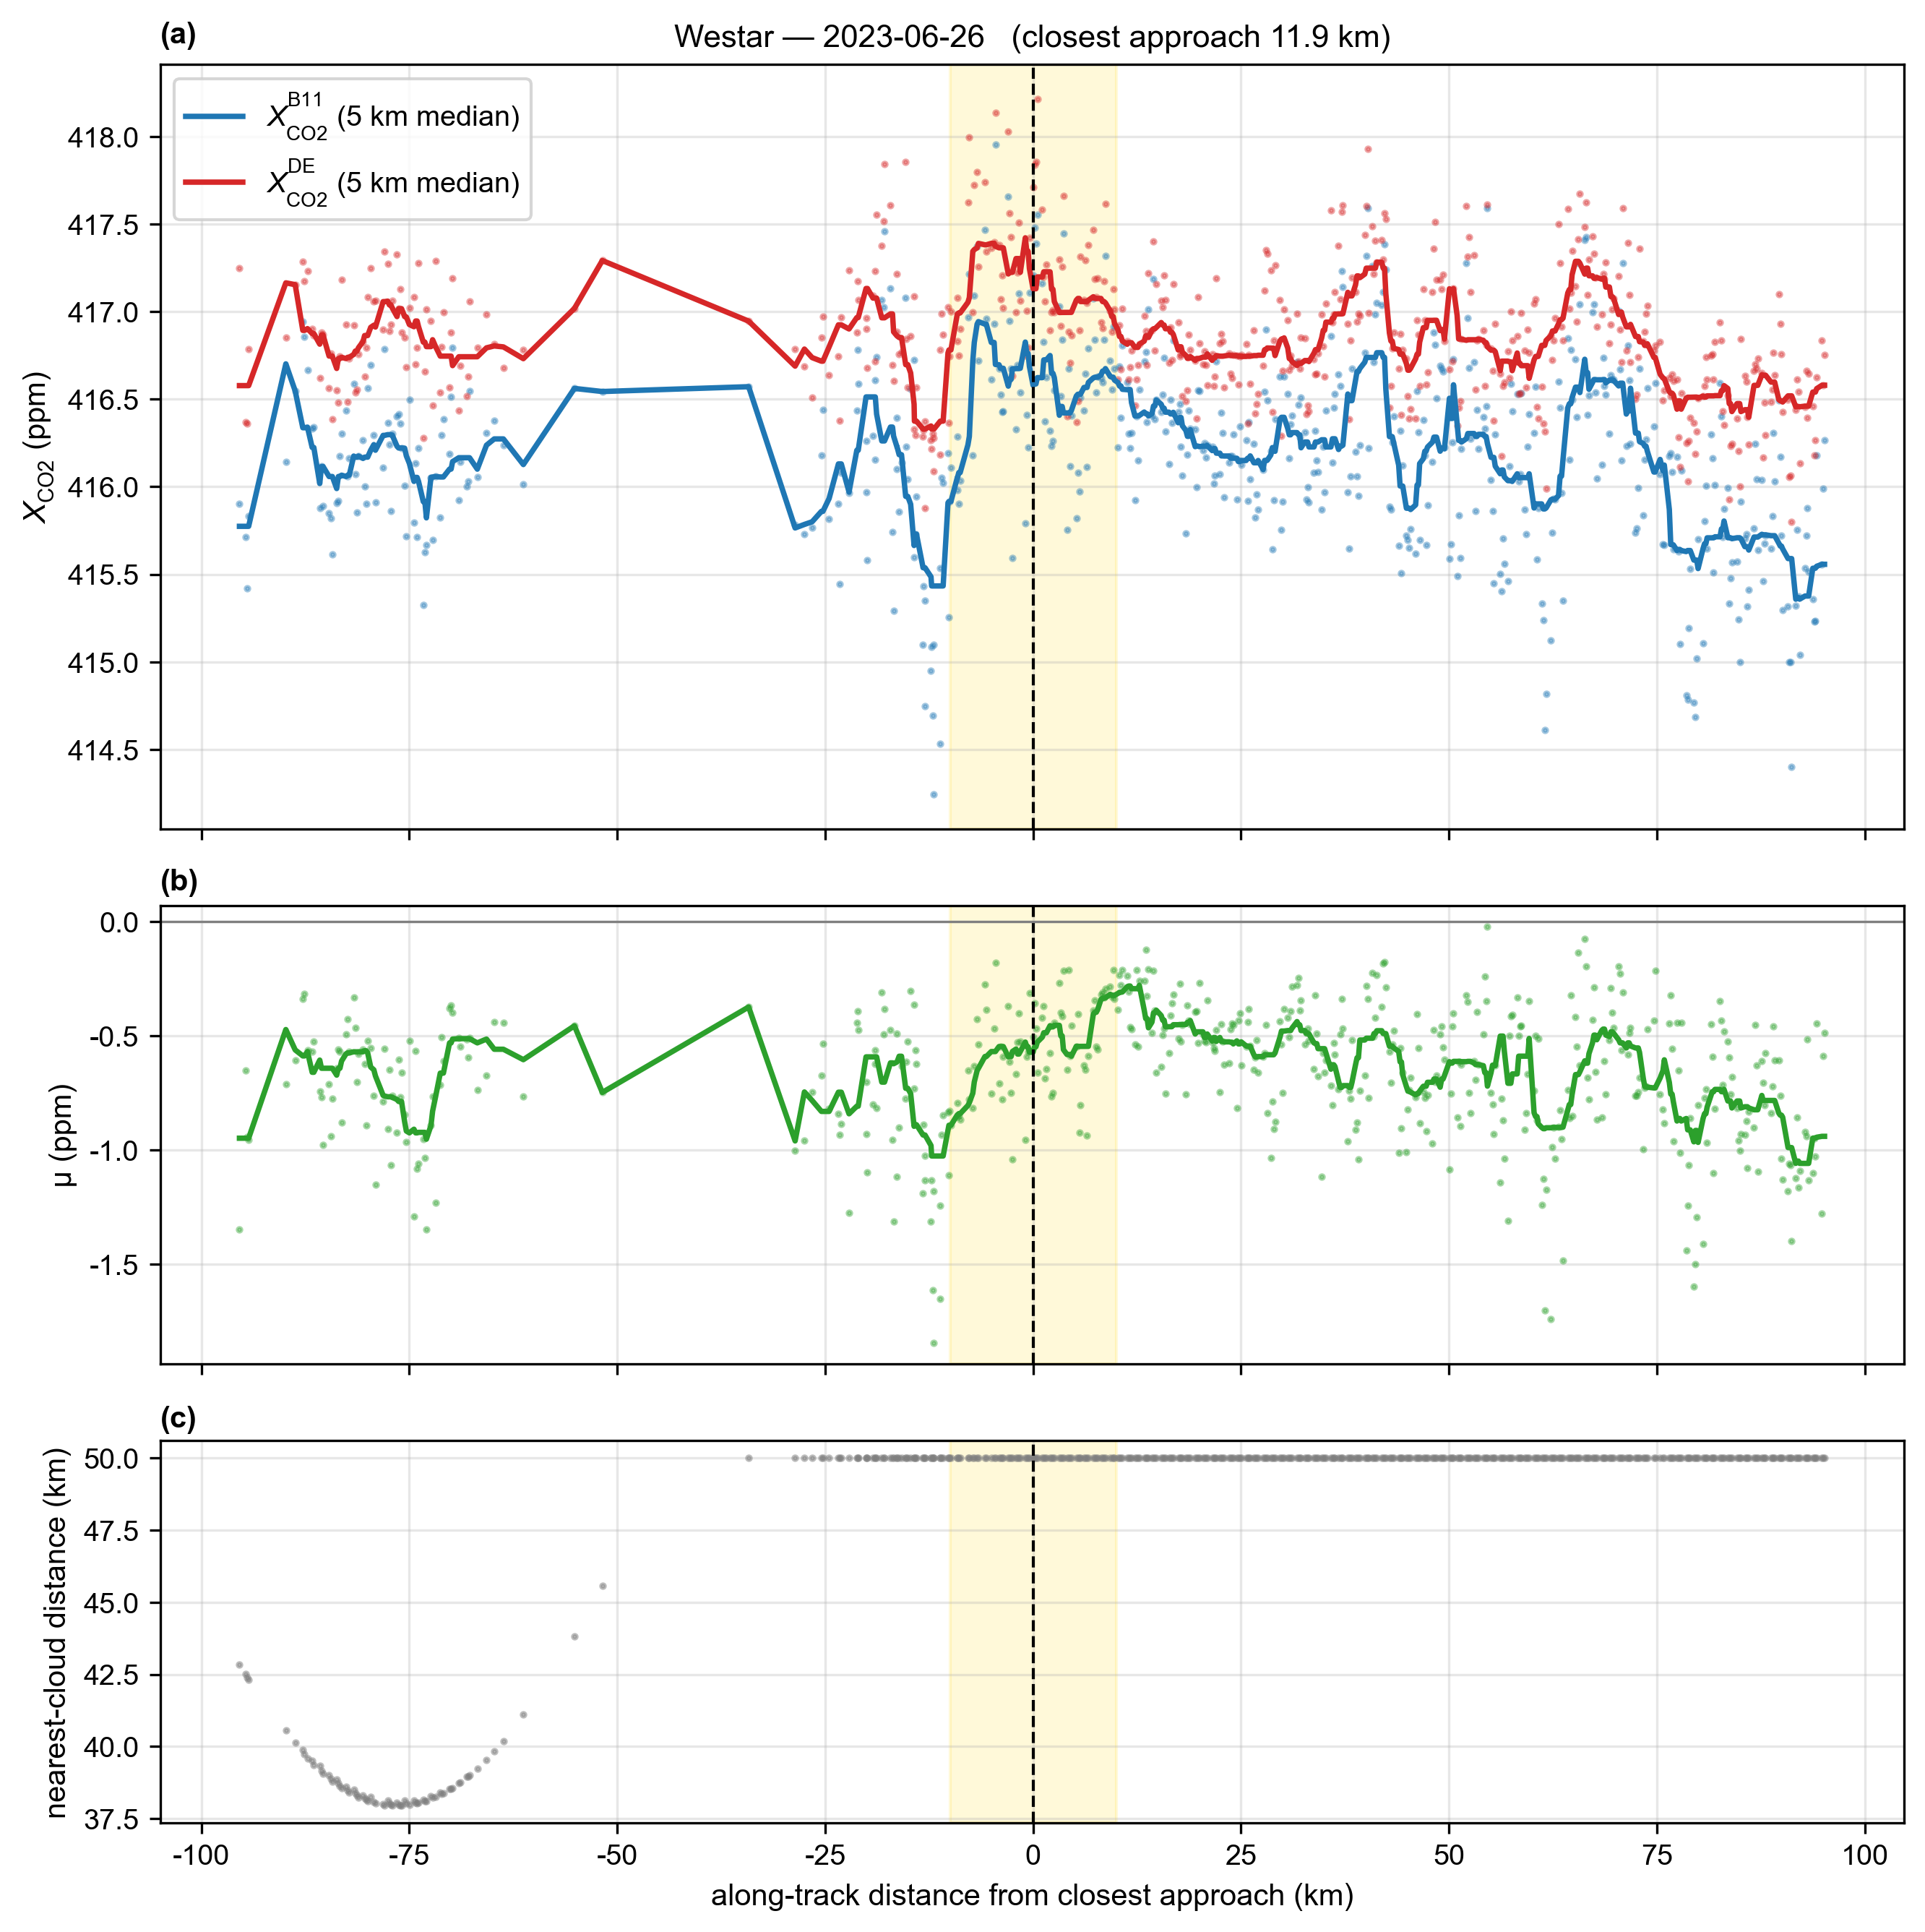
\includegraphics[width=0.65\textwidth]{figures/fig12a_westar_transect.png}\\[4pt]
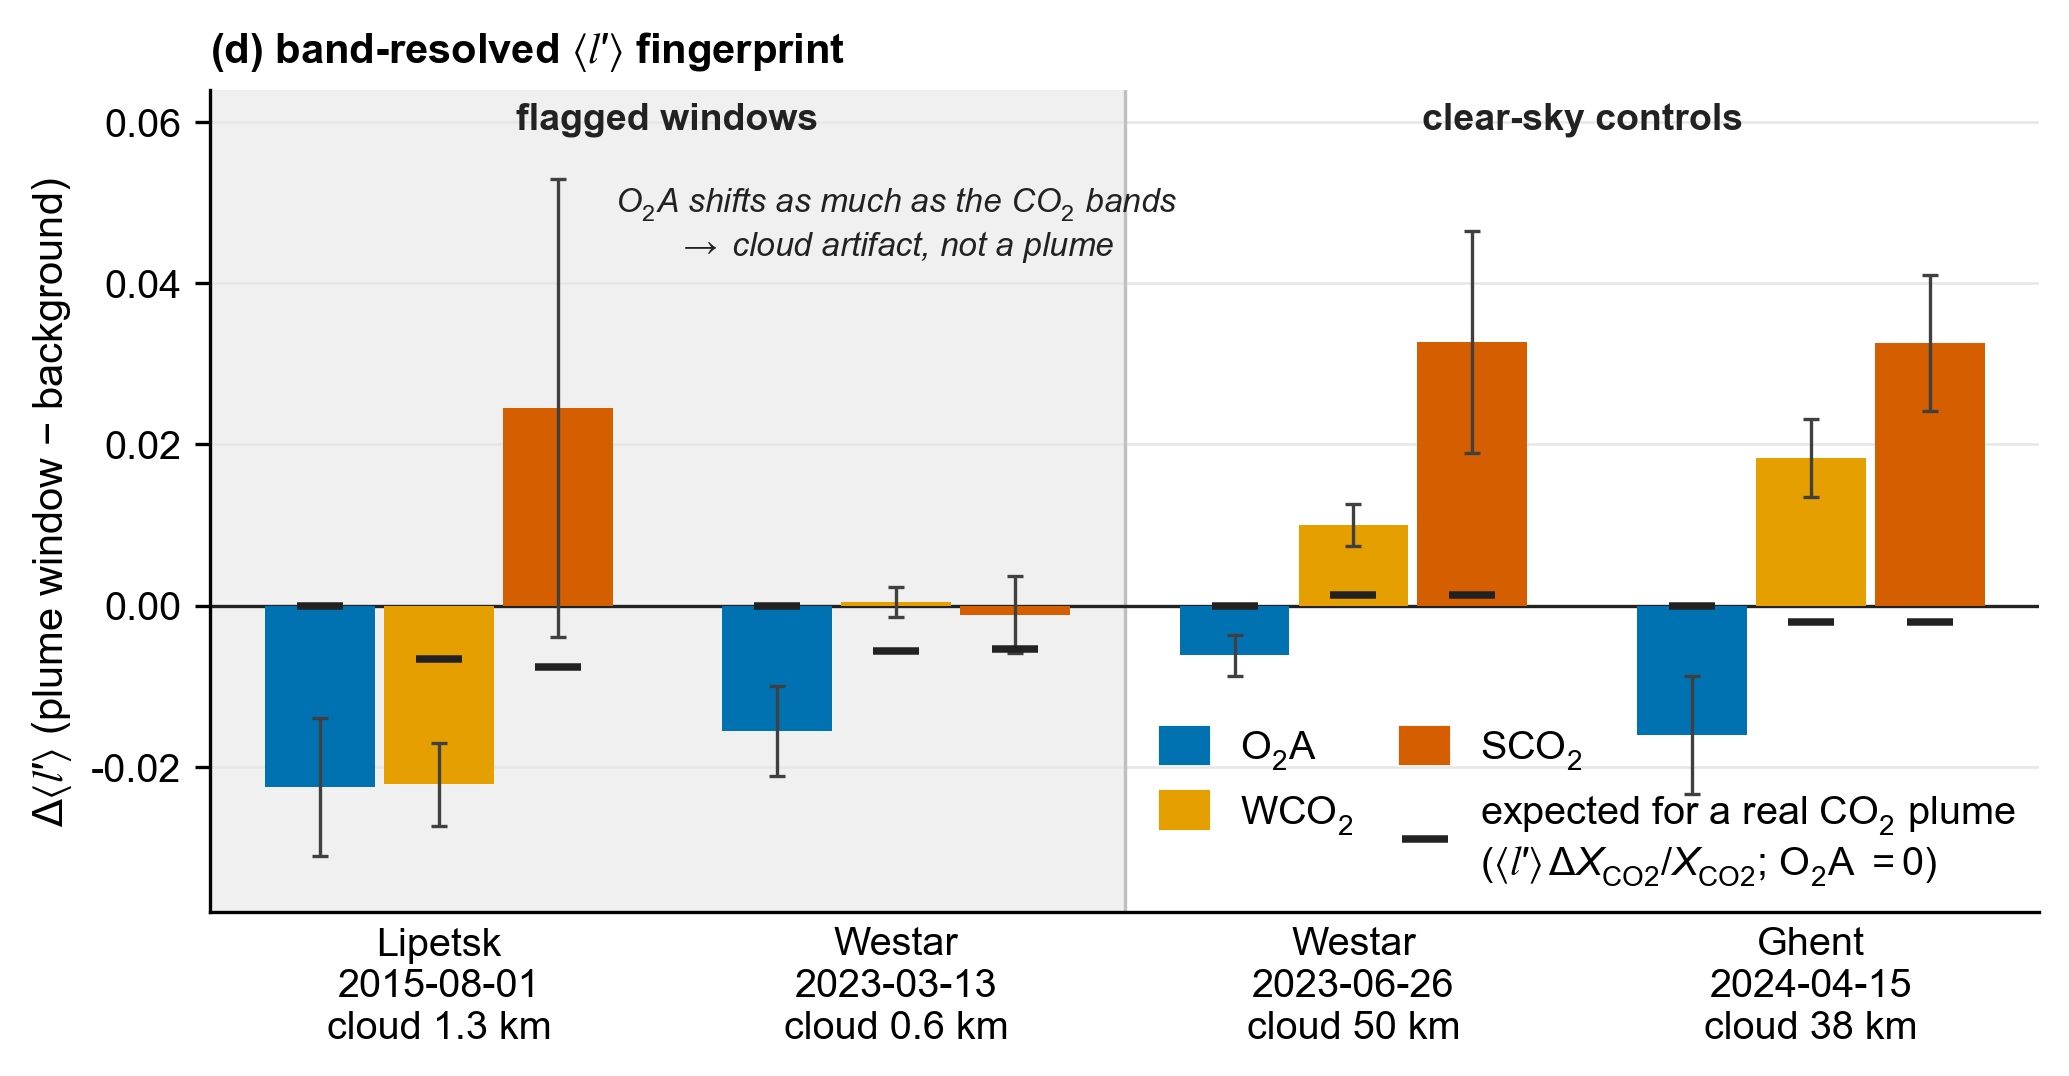
\includegraphics[width=0.65\textwidth]{figures/fig12b_k1_contrast.png}
\caption{Plume preservation and the spectral cloud fingerprint. (a) Along-track transect over the Westar power plant (26 June 2023, clear sky, nearest cloud ≈ 50 km; overpass from the Nassar et al. catalog) before and after correction; lower panels: predicted correction μ and nearest-cloud distance. (b) Band-resolved $\Delta$⟨$l'$⟩ (plume window minus background; ±1 SE) for the two flagged removal windows and two clear-sky controls. Black ticks: signature expected of a real CO2 plume ($\Delta$⟨$l'$⟩ ≈ ⟨$l'$⟩·$\Delta$\xco/\xco in the \ce{CO2} bands via the prior-based optical depth; exactly zero in \ce{O2}A).}
\label{fig:plume-preservation}
\end{figure}




\FloatBarrier

\subsection{Uncertainty and failure modes}
\label{sec:result-unc}




% 4.2 Spectral evidence for a common 3-D mechanism

% Build a three-part evidence chain:

% 1. band- and surface-resolved \(k_1/k_2\) responses with cloud distance;
% 2. the WCO2 land-cover sign rule: savanna approximately \(+0.43\sigma\) and
%    barren approximately \(-0.40\sigma\);
% 3. shadow and brightening branches with opposite XCO2 responses.

% Interpret ocean as the dark endpoint of the cloud–surface contrast axis, but
% label this as a synthesis supported by the observations rather than a closed
% quantitative derivation.

% Use the verified wording:

% > The sign of the WCO2 response follows the measured contrast where land
% > classes straddle the cloud albedo; response magnitudes do not monotonically
% > follow contrast.

% Do not use the superseded “forest sign flip” or “albedo-contrast ordering”
% claims. Close with one RGB case study; move category atlases to the Supplement.

% 4.3 Cross-validated correction performance

% Report random-split inflation versus date-blocked performance, land/ocean and
% near/far-cloud skill, label-noise ceilings, and uncertainty calibration.

% Interpret performance against the estimated ceiling rather than against
% \(R^2=1\): ocean global skill is approximately noise-limited, while land has
% remaining headroom concentrated in the near-cloud regime.

% 4.4 Model comparison and feature attribution

% Present the common-protocol baseline table, emphasizing the difficult
% near-cloud land tail. Then report:

% - the full ensemble performs best overall;
% - `no_spec` is approximately TCCON-neutral;
% - `no_xco2` degrades strongly, particularly for near-cloud land QF1;
% - spectral features remain conditionally informative when the XCO2-departure
%   block is removed.

% State the skill-versus-trust synthesis here for the first time.

% 4.5 Independent TCCON validation

% Use AK-harmonized TCCON as the primary reference and direct TCCON as a
% documented secondary comparison. Report the current production values only
% after regenerating the manuscript table from the frozen tag.

% The paragraph order should be:

% 1. sample and coincidence definition;
% 2. mean absolute bias and footprint RMSE;
% 3. number of improved station-days;
% 4. Wilcoxon and site-clustered bootstrap results;
% 5. radius/window and QF0/QF1 sensitivity;
% 6. high-latitude and worsening cases.

% Keep direct-reference results nearby but do not let the dual-reference
% explanation obscure the AK-harmonized primary result.

% 4.6 Distinguishing correction from smoothing

% Place the feature-free smoother immediately after TCCON:

% - it reduces footprint scatter more than the model;
% - it leaves station-day bias nearly unchanged;
% - the model reduces both bias and RMSE.

% This establishes that the validation improvement is not merely local
% denoising.

% 4.7 Ocean validation and far-cloud controls

% Present ATom, shipborne EM27/SUN, and the far-cloud/clear-day cases where the
% correction is nearly inert. Treat these as independent corroboration, not as
% equivalent in statistical weight to TCCON. State the limited sample and
% reference-scale caveats.

% 4.8 Plume preservation and correction safety

% Report:

% - matched control-window nulls;
% - the preserved Westar transect enhancement;
% - the all-band versus CO2-band \(k_1\) discriminator;
% - the spectral-channel removal bound of at most 0.21 ppm in the worst tested
%   case and at most 0.01 ppm in clear cases;
% - approximately 55% [40–63%] removal of plume-free local spread by the full
%   model, 54% by `no_spec`, and 29% by `no_xco2`.

% The required interpretation is:

% > Local smoothing is primarily attributable to the retrieval-state channel,
% > not to the photon path-length features.

% 4.9 Uncertainty and failure modes

% End Results by defining the boundary of reliability:

% - random-effects residual offset and its reference-scale interpretation;
% - representation error increasing with coincidence radius;
% - under-dispersed whole-budget uncertainty if between-case variance is
%   omitted;
% - bright surfaces as the main footprint-level failure stratum;
% - high-latitude residuals as station-day bias failures;
% - predictive uncertainty as a useful land-failure indicator that cannot
%   remove reference-scale bias.

\section{Discussion}

\input{5.1_physics_interp}

\input{5.2_opt_bc}

\input{5.3_imager_indepent}

\input{5.4_recovery}

\subsection{Limitations}
\label{sec:disc-limitation}


% 5.1 Physical interpretation

% Synthesize, rather than repeat, the land–ocean response, WCO2 sign rule, and
% shadow/brightening bifurcation. Explain why separate land and ocean models are
% physically justified. Distinguish the empirical mechanism evidence from full
% PPDF moment closure.



\input{5.6_future}

% 5.1 Physical interpretation

% Synthesize, rather than repeat, the land–ocean response, WCO2 sign rule, and
% shadow/brightening bifurcation. Explain why separate land and ocean models are
% physically justified. Distinguish the empirical mechanism evidence from full
% PPDF moment closure.

% 5.2 Relationship to the operational bias correction

% Discuss the raw/BC/ML experiment:

% - an ML model trained from raw retrievals recovers much of the operational
%   increment;
% - ML applied to bias-corrected XCO2 performs best overall;
% - near-cloud land is complementary: the operational correction can
%   over-correct, while the learned residual model partly reverses it.

% Frame the proposed method as a complementary residual correction, not a
% replacement for the operational correction.

% 5.3 Meaning and limits of imager independence

% Use three tiers:

% 1. **Deployment:** no imager or neighboring footprints at inference.
% 2. **Sensitivity:** the spectrum contains cloud-proximity information,
%    including a response below the MODIS resolution floor.
% 3. **Transferability:** the conceptual requirements are resolved absorption
%    bands, channel-level prior optical depth, and single-footprint spectra.

% State the caveat once:

% > The imager serves as scaffolding for target construction and validation but
% > is removed from the deployed correction.

% Discuss post-2022 OCO-2 use and OCO-3, CO2M, GOSAT-GW, and TEMPO as prospects,
% not demonstrated cross-sensor equivalence.

% 5.4 Observation-recovery implications

% Use production QF1 counts to quantify candidate recovery by distance, surface,
% and region. Avoid calling observations “usable” solely because RMSE is lower;
% formal acceptance also requires retrieval validity, uncertainty calibration,
% and downstream application tests.

% Recommended language is **candidates for recovery** until an explicit
% acceptance criterion and inversion experiment exist.

% 5.5 Limitations

% Collect the limitations in one subsection:

% - anomaly-target circularity and possible real-gradient contamination;
% - MYD35 mask semantics, sub-pixel cloud, and parallax limitations;
% - land-heavy TCCON sampling and limited ocean-reference sample;
% - high-latitude and representation-error residuals;
% - absence of fitted-versus-tallied PPDF moment closure;
% - possible attenuation of local CO2 contrast by retrieval-state predictors.

% #### 5.6 Future work

% Keep this short: Monte Carlo PPDF closure, plume-injection OSSE,
% transport-model decomposition of the target, cross-sensor validation, and a
% downstream flux-inversion assessment.

\conclusions  %% \conclusions[modified heading if necessary]


Use four short paragraphs:

1. Cloud adjacency produces coherent surface-dependent XCO2 and spectral
   responses.
2. Photon path-length statistics support a unified cloud–surface contrast
   interpretation.
3. A date-blocked, single-footprint probabilistic correction improves
   independent-reference agreement and outperforms smoothing.
4. Predictive skill comes mainly from retrieval-state variables, while the
   spectral physics provides interpretation, safety tests, and a route toward
   imager-free deployment.

Suggested final sentence:

> These results establish a practical route for correcting cloud-proximity
> errors without an imager at inference, while identifying the reference,
> surface, and representation-error limits that must accompany scientific
> applications.



%% The following commands are for the statements about the availability of data sets and/or software code corresponding to the manuscript.
%% It is strongly recommended to make use of these sections in case data sets and/or software code have been part of your research the article is based on.

\codeavailability{TEXT} %% use this section when having only software code available


\dataavailability{TEXT} %% use this section when having only data sets available


\codedataavailability{TEXT} %% use this section when having data sets and software code available


\sampleavailability{TEXT} %% use this section when having geoscientific samples available


\videosupplement{TEXT} %% use this section when having video supplements available



\appendix

%\appendixfigures

%\appendixtables 

\section{Spectral fitting and photon path-length derivation}
\label{app:spectral_fit_derivation}

%\subsection{}     %% Appendix A1, A2, etc.


The high-resolution vertical optical depth is computed from layer extinction as
\begin{equation}
\tau_v(\lambda_q)
=
\sum_z
\alpha(\lambda_q,z)\Delta z
+
\tau_{\mathrm{Ray}}(\lambda_q),
\label{eq:vertical_tau_hr}
\end{equation}
where $\alpha$ includes the target absorber and H$_2$O absorption on the ABSCO
grid, and $\tau_{\mathrm{Ray}}$ is the Rayleigh optical depth.


The high-resolution slant optical depth is
\begin{equation}
\mathrm{SOD}(\lambda_q)
=
\left(
\frac{1}{\cos\theta} + \frac{1}{\cos\phi}
\right)
\tau_v(\lambda_q).
\label{eq:hr_sod}
\end{equation}


Because the instrument line shape operates on transmission rather than optical
depth, the channel value used in the fit is
\begin{equation}
\overline{\mathrm{SOD}}_c
=
-\ln
\left[
\frac{
\sum_q R_{cq}\exp\{-\mathrm{SOD}(\lambda_q)\}
}{
\sum_q R_{cq}
}
\right].
\label{eq:discrete_ils_sod}
\end{equation}


The high-resolution solar spectrum is adjusted for Earth--Sun distance and the
solar Doppler stretch before convolution with the instrument line shape:
\begin{equation}
F_{\odot}^{\ast}(\lambda_q)
=
\frac{
F_{\odot}(\lambda_q)
}{
d_{\mathrm{AU}}^2
}
\frac{1}{1+\beta},
\qquad
\lambda_q^{\ast}
=
\lambda_q(1+\beta),
\label{eq:solar_distance_doppler}
\end{equation}
where $d_{\mathrm{AU}}$ is the Earth--Sun distance in astronomical units and
$\beta=v_{\mathrm{solar}}/c$.


The channel solar term is then computed as the ILS-weighted mean,
\begin{equation}
\mathcal{F}_{0,c}^{\mathrm{ILS}}
=
\frac{
\sum_q R_{cq}F_{\odot}^{\ast}(\lambda_q^{\ast})
}{
\sum_q R_{cq}
}.
\label{eq:solar_ils_convolution}
\end{equation}


\begin{equation}
\mathcal{F}_{0,c}
=
m_1
\mathcal{F}_{0,c}^{\mathrm{ILS}}
\frac{1}{\cos\theta},
\qquad
m_1 = 0.5,
\label{eq:effective_solar_normalization}
\end{equation}


\begin{equation}
T_c
=
\frac{\pi I_c}{\mathcal{F}_{0,c}}.
\label{eq:code_transmittance}
\end{equation}






For a photon traveling along the path coordinate $s$ over the total path length $L$, the Beer--Lambert transmittance is
\begin{equation}
T_{\lambda}(L)
=
\exp\left[
-
\int_0^L
\sigma_{\lambda}(s)n(s)
\,\mathrm{d}s
\right]
=
\exp\left[
-
\int_0^L
\alpha_{\lambda}(s)
\,\mathrm{d}s
\right],
\label{eq:beer_lambert_path}
\end{equation}



where $\alpha_{\lambda}(s)=\sigma_{\lambda}(s)n(s)$ is the absorption
coefficient. Averaging over photons with different path lengths gives
\begin{equation}
\bar{T}_{\lambda}
=
\frac{1}{N}
\sum_{i=1}^{N}
\exp\left[
-
\int_0^{L_i}
\alpha_{\lambda,i}(s)
\,\mathrm{d}s
\right].
\label{eq:ensemble_transmittance}
\end{equation}


Under the mean-absorption approximation,
$\alpha_{\lambda,i}(s)\approx\bar{\alpha}_{\lambda}$, so that
\begin{equation}
\bar{T}_{\lambda}
\approx
\frac{1}{N}
\sum_{i=1}^{N}
\exp(-\bar{\alpha}_{\lambda}L_i)
=
\int_0^\infty
p_L(L)
\exp(-\bar{\alpha}_{\lambda}L)
\,\mathrm{d}L .
\label{eq:path_length_laplace_dimensional}
\end{equation}

\begin{equation}
\overline{\mathrm{SOD}}_j
=
-\ln
\left[
\frac{
\sum_q R_j(\lambda_q)
\exp\{-\mathrm{SOD}(\lambda_q)\}
}{
\sum_q R_j(\lambda_q)
}
\right],
\end{equation}

where $j$ indexes the discrete wavelength samples in an OCO-2 band and
$q$ indexes the high-resolution wavelength grid used for the ILS convolution.


Let $\bar{L}$ be the direct geometric slant path and define the dimensionless
path-length enhancement
\begin{equation}
l' = \frac{L}{\bar{L}},
\qquad
\overline{\mathrm{SOD_{c, \lambda}}}
=
\bar{\alpha}_{\lambda}\bar{L}.
\label{eq:path_enhancement_tau}
\end{equation}



The ensemble transmittance can then be written as the Laplace transform of
the path-enhancement distribution:
\begin{equation}
\bar{T}(\overline{\mathrm{SOD}}_c)
=
\int_0^\infty
p(l')
\exp(-\overline{\mathrm{SOD}}_c \, l')
\,\mathrm{d}l' .
\label{eq:path_enhancement_laplace}
\end{equation}


For a Lambertian surface with reflectance $\gamma$,
\begin{equation}
\pi I_c(\lambda)
=
\mathcal{F}_{0,c}(\lambda)\cos\theta\,
\gamma\,
\bar{T}(\overline{\mathrm{SOD}}_{c \, \lambda}),
\label{eq:radiance_lambertian}
\end{equation}



and therefore
\begin{equation}
T(\overline{\mathrm{SOD}}_c)
\equiv
\frac{\pi I_c}{\mathcal{F}_{0,c}\cos\theta}
=
\gamma
\int_0^\infty
p(l')
\exp(-\overline{\mathrm{SOD}}_c \, l')
\,\mathrm{d}l' .
\label{eq:measured_laplace_appendix}
\end{equation}



If $p(l')$ is approximated by a gamma distribution with mean
$\mu_{l'}=\langle l'\rangle$ and shape parameter
$\kappa=\mu_{l'}^2/\operatorname{var}(l')$, then
\begin{equation}
p(l')
=
\frac{(\kappa/\mu_{l'})^{\kappa}}{\Gamma(\kappa)}
l'^{\kappa-1}
\exp\left(-\frac{\kappa}{\mu_{l'}}l'\right),
\qquad
l' \ge 0 .
\label{eq:gamma_path_distribution}
\end{equation}



Its Laplace transform is
\begin{equation}
\int_0^\infty
p(l')\exp(-\overline{\mathrm{SOD}}_c \, l')
\,\mathrm{d}l'
=
\left(
1+\frac{\mu_{l'}}{\kappa}\overline{\mathrm{SOD}}_c
\right)^{-\kappa},
\label{eq:gamma_laplace_transform}
\end{equation}



so the measured transmittance is
\begin{equation}
T(\overline{\mathrm{SOD}}_c)
=
\gamma
\left(
1+\frac{\mu_{l'}}{\kappa}\overline{\mathrm{SOD}}_c
\right)^{-\kappa}.
\label{eq:gamma_transmittance}
\end{equation}



Taking the logarithm gives
\begin{equation}
\ln T(\overline{\mathrm{SOD}}_c)
=
\ln\gamma
-
\kappa
\ln\left(
1+\frac{\mu_{l'}}{\kappa}\overline{\mathrm{SOD}}_c
\right).
\label{eq:log_gamma_transmittance}
\end{equation}


Using the Taylor expansion of the logarithm,
\begin{equation}
\ln T(\overline{\mathrm{SOD}}_c)
=
\ln\gamma
-
\mu_{l'}\overline{\mathrm{SOD}}_c
+
\frac{\mu_{l'}^2}{2\kappa}\overline{\mathrm{SOD}}_c^2
-
\frac{\mu_{l'}^3}{3\kappa^2}\overline{\mathrm{SOD}}_c^3
+
\cdots .
\label{eq:log_gamma_taylor}
\end{equation}



The fitted polynomial is written as
\begin{equation}
\ln T(\overline{\mathrm{SOD}}_c)
=
b
+
\sum_{n=1}^{N}
(-1)^n
\frac{k_n}{n}
\overline{\mathrm{SOD}}_c^n,
\qquad
b=\ln\gamma .
\label{eq:log_polynomial_fit_appendix}
\end{equation}



For the gamma model, matching coefficients gives
\begin{equation}
k_n
=
\frac{\mu_{l'}^{n}}{\kappa^{n-1}},
\qquad
n\ge 1 .
\label{eq:gamma_coefficient_identity}
\end{equation}




Thus
\begin{equation}
k_1=\mu_{l'},
\qquad
k_2=\frac{\mu_{l'}^{2}}{\kappa}
=
\operatorname{var}(l'),
\qquad
\kappa=\frac{k_1^2}{k_2}.
\label{eq:k1_k2_kappa_identity}
\end{equation}

\section{Data provenance, cloud collocation, and target construction}
\label{app:data}





\section{Model architecture, training, and reproducibility}
\label{app:model}



\subsection{Deep-ensemble Member architecture and probabilistic head}

Each of the $M = 5$ ensemble members is a Gaussian-head multilayer perceptron
with two hidden layers (64 and 32 units). Every hidden block applies, in order,
a linear map, layer normalization, a ReLU activation, and 10\% dropout; dropout
is active during training only, so there is no Monte-Carlo dropout at inference
and the ensemble spread alone provides the epistemic uncertainty. For footprint
$i$, member $m$ outputs a predicted mean $\mu_{m,i}$ and a raw second output that is clamped to $[-10, 10]$ and interpreted as the log-variance
$s_{m,i} = \log\sigma_{m,i}^{2}$, giving a per-footprint predictive variance
$\sigma_{m,i}^{2} = \exp(s_{m,i})$.

\subsection{Training loss}

Writing the target as $y_i \equiv \Delta \mathrm{X_{CO2,\,i}^{B11}}$, the standard
Gaussian negative log-likelihood of one footprint is, up to an additive constant,
%
\begin{equation}
  \ell^{\mathrm{NLL}}_{m,i}
  = \frac{1}{2}\left[\,s_{m,i}
  + \frac{(y_i-\mu_{m,i})^{2}}{\sigma_{m,i}^{2}}\,\right].
  \label{eq:gauss-nll}
\end{equation}
%
Because this loss down-weights high-variance footprints, the mean is poorly
fitted exactly in the near-cloud regime where $\sigma_{m,i}^{2}$ is large. We
therefore train the members with the $\beta$-NLL loss of
\citet{seitzer2022pitfalls}, which multiplies each footprint's NLL by a
stop-gradient function of its own predicted variance,
%
\begin{equation}
  \ell^{\beta\text{-}\mathrm{NLL}}_{m,i}
  = \bigl\lfloor\sigma_{m,i}^{2}\bigr\rfloor_{\mathrm{sg}}^{\,\beta}\;
  \ell^{\mathrm{NLL}}_{m,i},
  \qquad \beta = 0.5,
  \label{eq:beta-nll}
\end{equation}
%
where $\lfloor\cdot\rfloor_{\mathrm{sg}}$ denotes a stop-gradient (the weight is
treated as a constant during backpropagation). Here $\beta = 0$ recovers the
plain NLL of Eq.~\eqref{eq:gauss-nll} and $\beta = 1$ recovers a
mean-squared-error weighting of the mean; the production choice $\beta = 0.5$
restores the mean-fitting gradient in the high-variance near-cloud footprints
while keeping a calibrated variance. The member loss is the average of
Eq.~\eqref{eq:beta-nll} over the training footprints.

\subsection{Ensemble aggregation}

The five members differ only in their random seed (member $m$ uses seed
$s_0 + m$), so their predictions decorrelate and the ensemble spread provides
the epistemic uncertainty. The per-member means and variances are combined as a
Gaussian mixture,
%
\begin{equation}
  \mu^{*}_i = \frac{1}{M}\sum_{m=1}^{M}\mu_{m,i},
  \qquad
  \sigma^{*2}_i
  = \underbrace{\frac{1}{M}\sum_{m=1}^{M}\sigma_{m,i}^{2}}_{\text{aleatoric}}
  + \underbrace{\frac{1}{M}\sum_{m=1}^{M}\mu_{m,i}^{2} - \mu^{*2}_i}_{\text{epistemic}},
  \label{eq:mixture}
\end{equation}
%
which is the law of total variance: the first term is the mean aleatoric
variance predicted by the heads and the second is the between-member (epistemic)
variance. The ensemble mean $\mu^{*}_i$ is the point correction applied to each
footprint.

\subsection{Optimization and leakage control}

Each member is optimized with AdamW (learning rate $10^{-3}$, weight decay
$10^{-4}$) under a one-cycle learning-rate schedule with gradient-norm clipping
at $1.0$, a batch size of $4096$, and up to $500$ epochs. Training is stopped
early on the held-out calibration block (patience of $50$ epochs), and the
checkpoint with the lowest calibration loss is kept; the calibration block is
carved from the training dates and never overlaps the held-out fold or the
validation references. The calibration block is also used to recalibrate the
Mondrian conformal intervals, which are binned by predicted-anomaly deciles.
Feature scaling and any profile-EOF transforms are fitted on the proper-training
partition only. Table~\ref{tab:hyperparams} collects the full configuration.

\begin{table}[t]
\centering
\caption{DE-MLP architecture and training configuration (production settings).}
\label{tab:hyperparams}
\begin{tabular}{@{}ll@{}}
\toprule
Component & Setting \\
\midrule
Ensemble members $M$        & 5 (seeds $s_0 + m$) \\
Hidden layers               & 64, 32 \\
Hidden block                & Linear $\to$ LayerNorm $\to$ ReLU $\to$ Dropout(0.1) \\
Output head                 & Linear $\to$ 2 (mean, log-variance) \\
Log-variance clamp          & $[-10, 10]$ \\
Loss                        & $\beta$-NLL, $\beta = 0.5$ \\
Optimizer                   & AdamW \\
Learning rate (max)         & $10^{-3}$ \\
Weight decay                & $10^{-4}$ \\
LR schedule                 & one-cycle (\texttt{pct\_start} 0.05, div 25, final div 1000) \\
Gradient clipping           & 1.0 (max norm) \\
Batch size                  & 4096 \\
Maximum epochs              & 500 \\
Early stopping              & patience 50, on the calibration block \\
Calibration fraction        & 0.15 of the training dates \\
Conformal intervals         & Mondrian, 10 predicted-anomaly decile bins \\
\bottomrule
\end{tabular}
\end{table}


\subsection{Loss function for \emph{Ridge} and \emph{XGBoost} models}

The LR and XGBoost models are trained with the following objectives, all on the same target $y_i \equiv \Delta \mathrm{X_{CO2,\,i}^{B11}}$ and the same
train-only-standardized features $\mathbf{x}_i$.

\subsubsection*{Ridge} 
A linear predictor $\hat{y}_i = \mathbf{x}_i^{\top}\bm{\beta}$
trained by $\ell_2$-penalized least squares,
%
\begin{equation}
  \mathcal{L}_{\mathrm{Ridge}}(\bm{\beta})
  = \sum_i \bigl(y_i - \mathbf{x}_i^{\top}\bm{\beta}\bigr)^{2}
  + \alpha\,\lVert\bm{\beta}\rVert_{2}^{2},
  \label{eq:ridge}
\end{equation}
%
with the penalty $\alpha$ selected from $\{0.1, 1, 10, 100\}$ by lowest RMSE on
the calibration block.

\subsection*{XGBoost} 
A gradient-boosted tree ensemble
$\hat{y}_i = \sum_{t} f_t(\mathbf{x}_i)$ minimizing a regularized squared-error
objective,
%
\begin{equation}
  \mathcal{L}_{\mathrm{XGB}}
  = \sum_i \bigl(y_i - \hat{y}_i\bigr)^{2}
  + \sum_t \Omega(f_t),
  \qquad
  \Omega(f) = \tfrac{1}{2}\lambda\lVert w \rVert_{2}^{2},
  \label{eq:xgb}
\end{equation}
%
where $\Omega$ penalizes the leaf weights $w$ ($\lambda = 1$) and the number of
boosting rounds is early-stopped on the calibration block (maximum tree depth
$6$).

% \paragraph{DE-MLP.} Each of the $M = 5$ members minimizes the mean $\beta$-NLL
% loss of Eq.~\eqref{eq:beta-nll}; the ensemble prediction follows
% Eq.~\eqref{eq:mixture}.


\subsection{Model Predictors}

% Auto-generated by make_appendix_c_figures.py — do not hand-edit.
\begingroup\footnotesize
\begin{longtable}{lccp{0.50\linewidth}}
\caption{Full predictor inventory of the per-surface correction models (ocean: 56 inputs; land: 67), generated from the feature pipeline source. All quantities are per-sounding OCO-2 L2 Lite columns except the spectral path-length block (fitted from the L1B spectrum, Sect.~3.2) and the profile-EOF block (fold-fitted PCA of the Lite meteorology/prior profiles). Sfc: which surface model uses the feature. Transform: RS $=$ robust--standard scaling (median/IQR, then standardization), log1p applied first where marked; SS $=$ block-own standard scaler; both fitted on the training split only. Cloud distance is not an input.}
\label{tab:predictor-inventory}\\
\tophline
Feature & Sfc & Transform & Description \\
\middlehline
\endfirsthead
\multicolumn{4}{l}{\textit{(continued)}}\\
\tophline
Feature & Sfc & Transform & Description \\
\middlehline
\endhead
\bottomhline
\endfoot
\bottomhline
\multicolumn{4}{p{0.9\linewidth}}{\footnotesize The three named ablation groups of Table~2 map exactly onto the groups above: $-$xco2 drops the retrieval-state row, $-$spec the spectral path-length block, $-$contam the contamination-indicator block.}\\
\endlastfoot
\multicolumn{4}{l}{\textit{Retrieval state}} \\
\texttt{xco2\_raw\_minus\_apriori} & O$+$L & RS & Retrieved (pre-bias-correction) XCO$_2$ minus prior XCO$_2$ (ppm) \\
\middlehline
\multicolumn{4}{l}{\textit{Spectral path-length}} \\
\texttt{exp\_o2a\_intercept} & O$+$L & RS & O$_2$A continuum reflectance (exponential of the cumulant-fit intercept) \\
\texttt{o2a\_exp\_intercept-alb} & O$+$L & RS & O$_2$A continuum reflectance minus retrieved O$_2$A albedo \\
\texttt{o2a\_k1\_nosg} & O$+$L & RS & O$_2$A mean relative photon path $\langle l'\rangle$ (this work, Sect.~3.2) \\
\texttt{o2a\_k2\_nosg} & O$+$L & RS & O$_2$A photon-path variance $\mathrm{var}(l')$ \\
\texttt{wco2\_k1\_nosg} & O$+$L & RS & WCO$_2$ $\langle l'\rangle$ \\
\texttt{wco2\_k2\_nosg} & O$+$L & RS & WCO$_2$ $\mathrm{var}(l')$ \\
\texttt{wco2\_k3\_nosg} & O$+$L & RS & WCO$_2$ third-order path-length cumulant \\
\texttt{sco2\_k1\_nosg} & O$+$L & RS & SCO$_2$ $\langle l'\rangle$ \\
\texttt{sco2\_k2\_nosg} & O$+$L & RS & SCO$_2$ $\mathrm{var}(l')$ \\
\texttt{wco2\_exp\_intercept-alb} & L & RS & WCO$_2$ continuum reflectance minus retrieved WCO$_2$ albedo \\
\middlehline
\multicolumn{4}{l}{\textit{Geometry \& L1B diagnostics}} \\
\texttt{fp\_area\_km2} & O$+$L & log1p$+$RS & Footprint area (km$^2$) \\
\texttt{cos\_glint\_angle} & O & RS & Cosine of the glint angle \\
\texttt{h2o\_ratio\_bc} & O$+$L & RS & IDP H$_2$O band-ratio cloud-screen diagnostic (bias-corrected) \\
\texttt{csnr\_sco2} & O & RS & Continuum signal-to-noise ratio, SCO$_2$ band \\
\texttt{pol\_ang\_rad} & O$+$L & RS & Polarization angle (rad) \\
\texttt{s31} & O$+$L & RS & Band signal ratio SCO$_2$/O$_2$A \\
\texttt{1\_over\_cos\_sza} & L & RS & Solar air-mass factor $1/\cos(\mathrm{SZA})$ \\
\texttt{1\_over\_cos\_vza} & L & RS & Viewing air-mass factor $1/\cos(\mathrm{VZA})$ \\
\texttt{sin\_raa} & L & RS & Sine of the relative azimuth angle \\
\texttt{co2\_ratio\_bc} & L & RS & IDP CO$_2$ band-ratio cloud-screen diagnostic (bias-corrected) \\
\texttt{csnr\_o2a} & L & RS & Continuum signal-to-noise ratio, O$_2$A band \\
\texttt{h\_cont\_o2a} & L & RS & O$_2$A continuum-radiance variability across adjacent soundings (per-sounding preprocessor value) \\
\texttt{h\_cont\_sco2} & L & RS & SCO$_2$ continuum-radiance variability across adjacent soundings \\
\middlehline
\multicolumn{4}{l}{\textit{Meteorology, surface \& aerosol}} \\
\texttt{log\_P} & O$+$L & RS & Log of retrieved surface pressure \\
\texttt{dp\_psfc\_prior\_ratio} & O$+$L & RS & Retrieved-minus-prior surface pressure, relative to the prior \\
\texttt{h2o\_scale} & O$+$L & RS & Retrieved H$_2$O-profile scale factor \\
\texttt{delT} & O$+$L & RS & Retrieved temperature-profile offset (K) \\
\texttt{co2\_grad\_del} & O$+$L & RS & Change in the retrieved CO$_2$ vertical gradient relative to the prior \\
\texttt{aod\_dust} & O$+$L & log1p$+$RS & Retrieved dust aerosol optical depth \\
\texttt{aod\_oc} & O$+$L & log1p$+$RS & Retrieved organic-carbon aerosol optical depth \\
\texttt{aod\_seasalt} & O$+$L & log1p$+$RS & Retrieved sea-salt aerosol optical depth \\
\texttt{aod\_strataer} & O$+$L & log1p$+$RS & Retrieved stratospheric-aerosol optical depth \\
\texttt{aod\_sulfate} & O$+$L & log1p$+$RS & Retrieved sulfate aerosol optical depth \\
\texttt{tcwv} & O$+$L & RS & Total column water vapour \\
\middlehline
\multicolumn{4}{l}{\textit{Contamination indicators}} \\
\texttt{max\_declock\_wco2} & O & RS & Maximum WCO$_2$ declocking correction (detector diagnostic) \\
\texttt{aod\_water} & O$+$L & log1p$+$RS & Retrieved water-cloud optical depth \\
\texttt{dp\_abp} & O$+$L & RS & A-band-preprocessor surface-pressure difference (cloud screen) \\
\texttt{h\_cont\_wco2} & O$+$L & RS & WCO$_2$ continuum-radiance variability across adjacent soundings \\
\texttt{t700} & O$+$L & RS & Temperature at 700\,hPa (K) \\
\texttt{water\_height} & O$+$L & RS & Retrieved water-cloud layer height \\
\texttt{alb\_sco2\_over\_wco2} & O$+$L & RS & Retrieved albedo ratio SCO$_2$/WCO$_2$ \\
\texttt{dpfrac} & L & RS & Fractional retrieved-minus-prior surface-pressure difference \\
\texttt{fs\_rel\_0} & L & RS & Relative fluorescence signal (clamped $\geq 0$) \\
\texttt{dust\_height} & L & RS & Retrieved dust layer height \\
\texttt{aod\_ice} & L & log1p$+$RS & Retrieved ice-cloud optical depth \\
\texttt{ice\_height} & L & RS & Retrieved ice-cloud layer height \\
\texttt{alt\_std} & L & RS & Std.\ dev.\ of surface altitude within the footprint (roughness) \\
\middlehline
\multicolumn{4}{l}{\textit{Footprint}} \\
\texttt{fp\_0}\,\ldots\,\texttt{fp\_7} & O$+$L & none & Footprint-index one-hot (8 across-track positions) \\
\middlehline
\multicolumn{4}{l}{\textit{Profile EOFs (appended block)}} \\
\texttt{t\_pc01}--\texttt{t\_pc04} & O$+$L & SS & Temperature-profile EOF scores ($\sigma$-grid, per surface) \\
\texttt{q\_pc01}--\texttt{q\_pc04} & O$+$L & SS & Specific-humidity EOF scores (log-compressed $\sigma$-grid) \\
\texttt{co2prior\_pc01}--\texttt{co2prior\_pc04} & O$+$L & SS & Shape-normalized prior-CO$_2$-profile EOF scores \\
\texttt{tropopause\_sigma} & O$+$L & SS & Tropopause pressure in $\sigma$ coordinate \\
\texttt{tropopause\_temp} & O$+$L & SS & Tropopause temperature (K) \\
\end{longtable}
\endgroup




\subsection{Data split}



%
\begin{figure}[t]
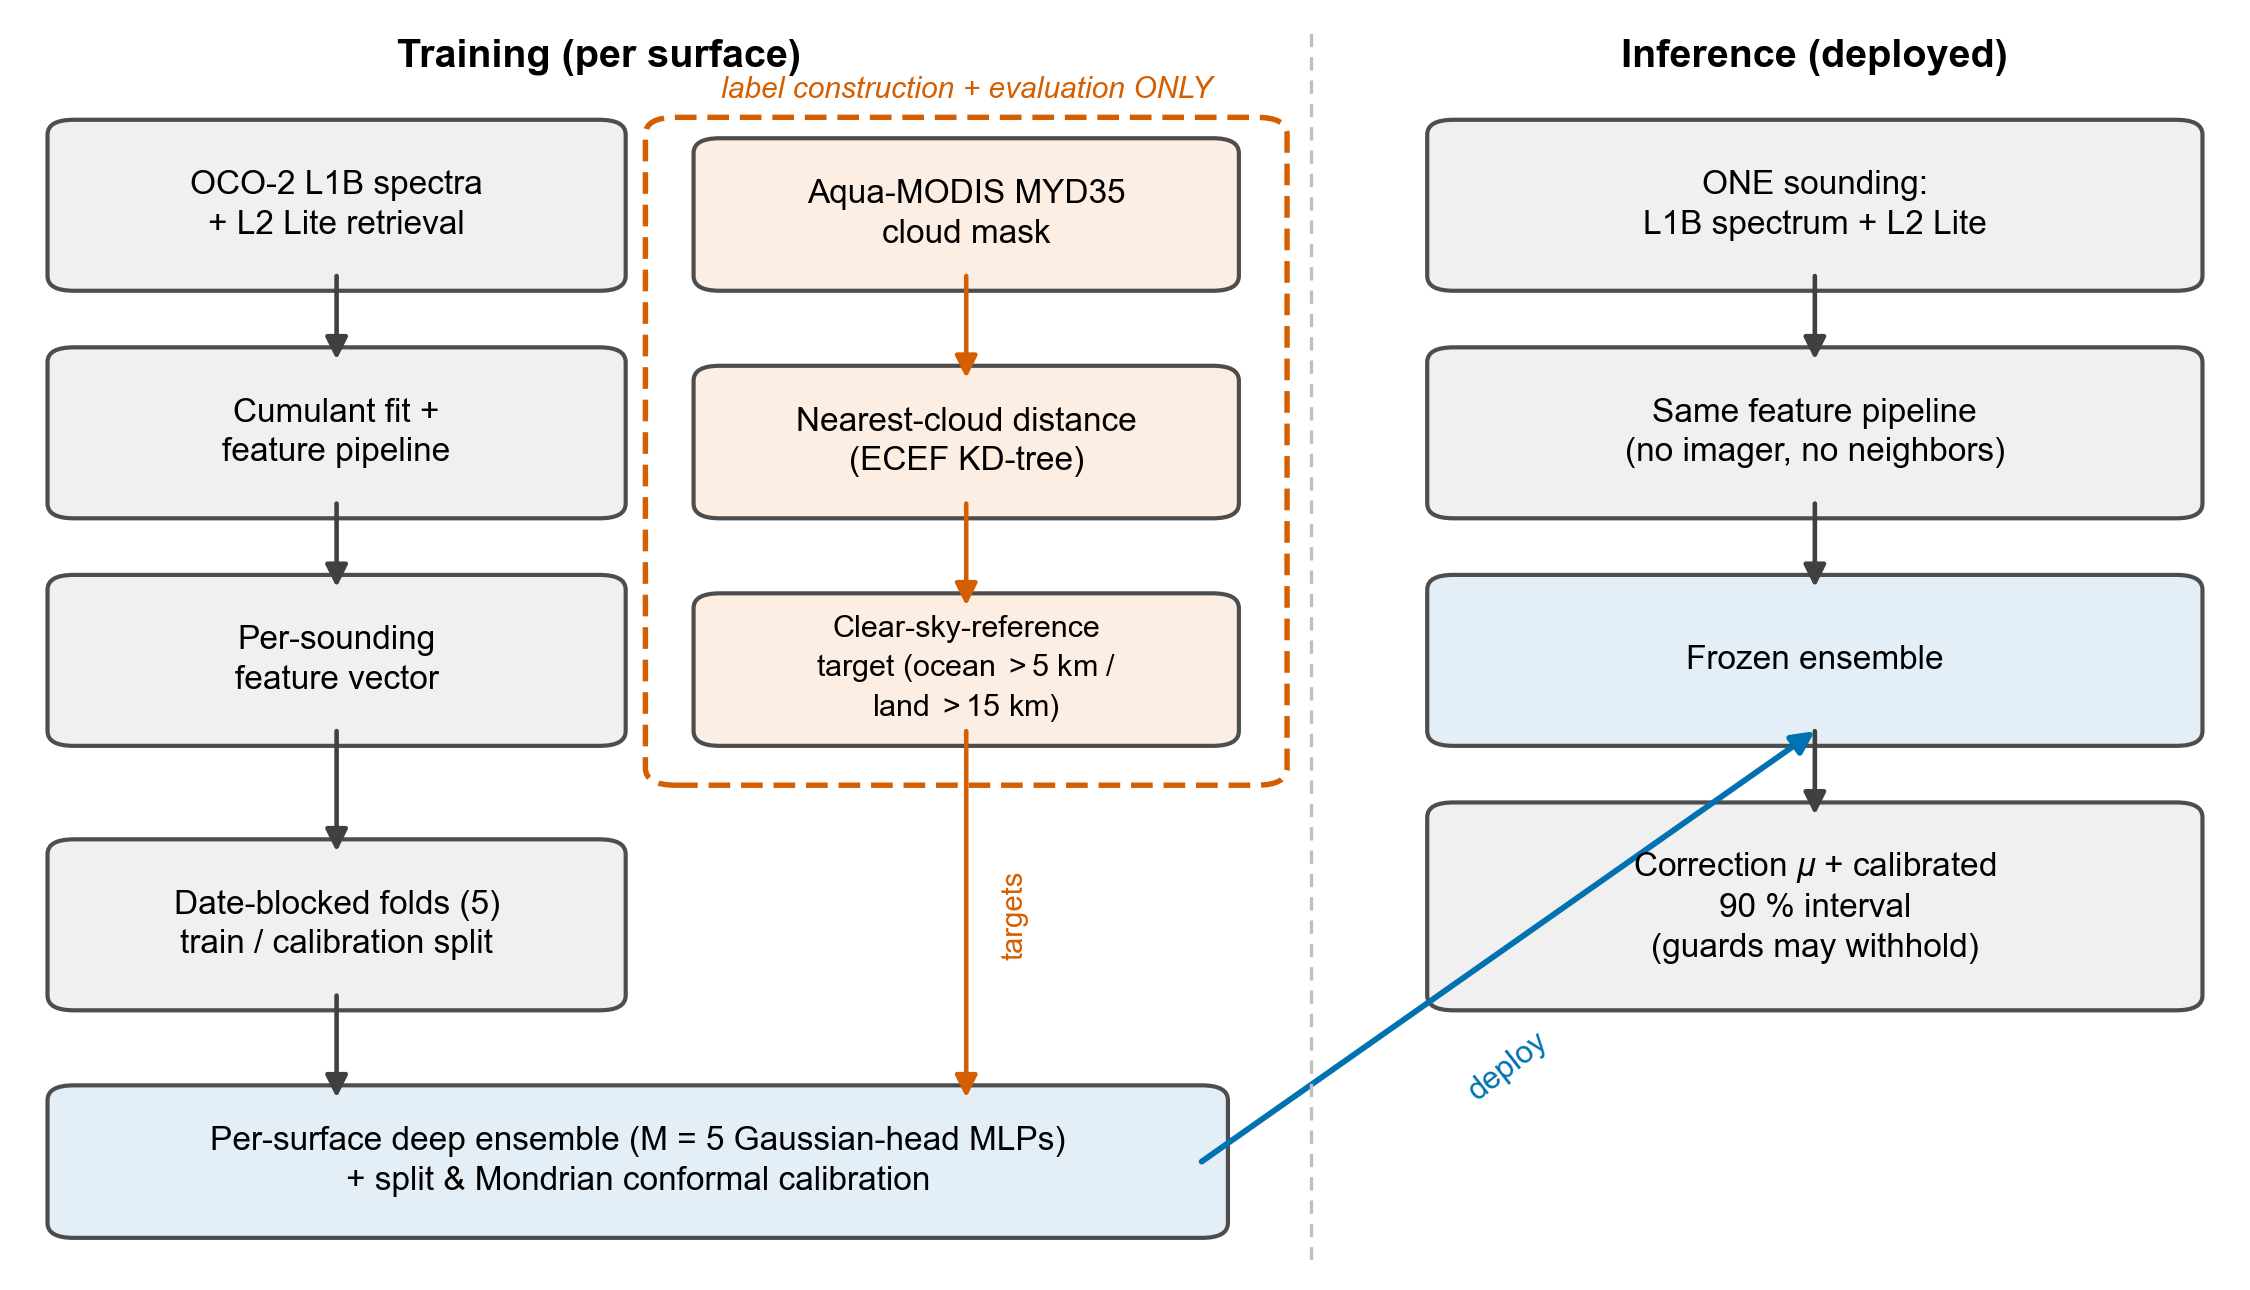
\includegraphics[width=\textwidth]{figures/figC1_dataflow.png}
\caption{Scheme of the data flow from training to inference/bias correction.}
\label{fig:train_infer_flow}
\end{figure}
%

\begin{figure}[t]
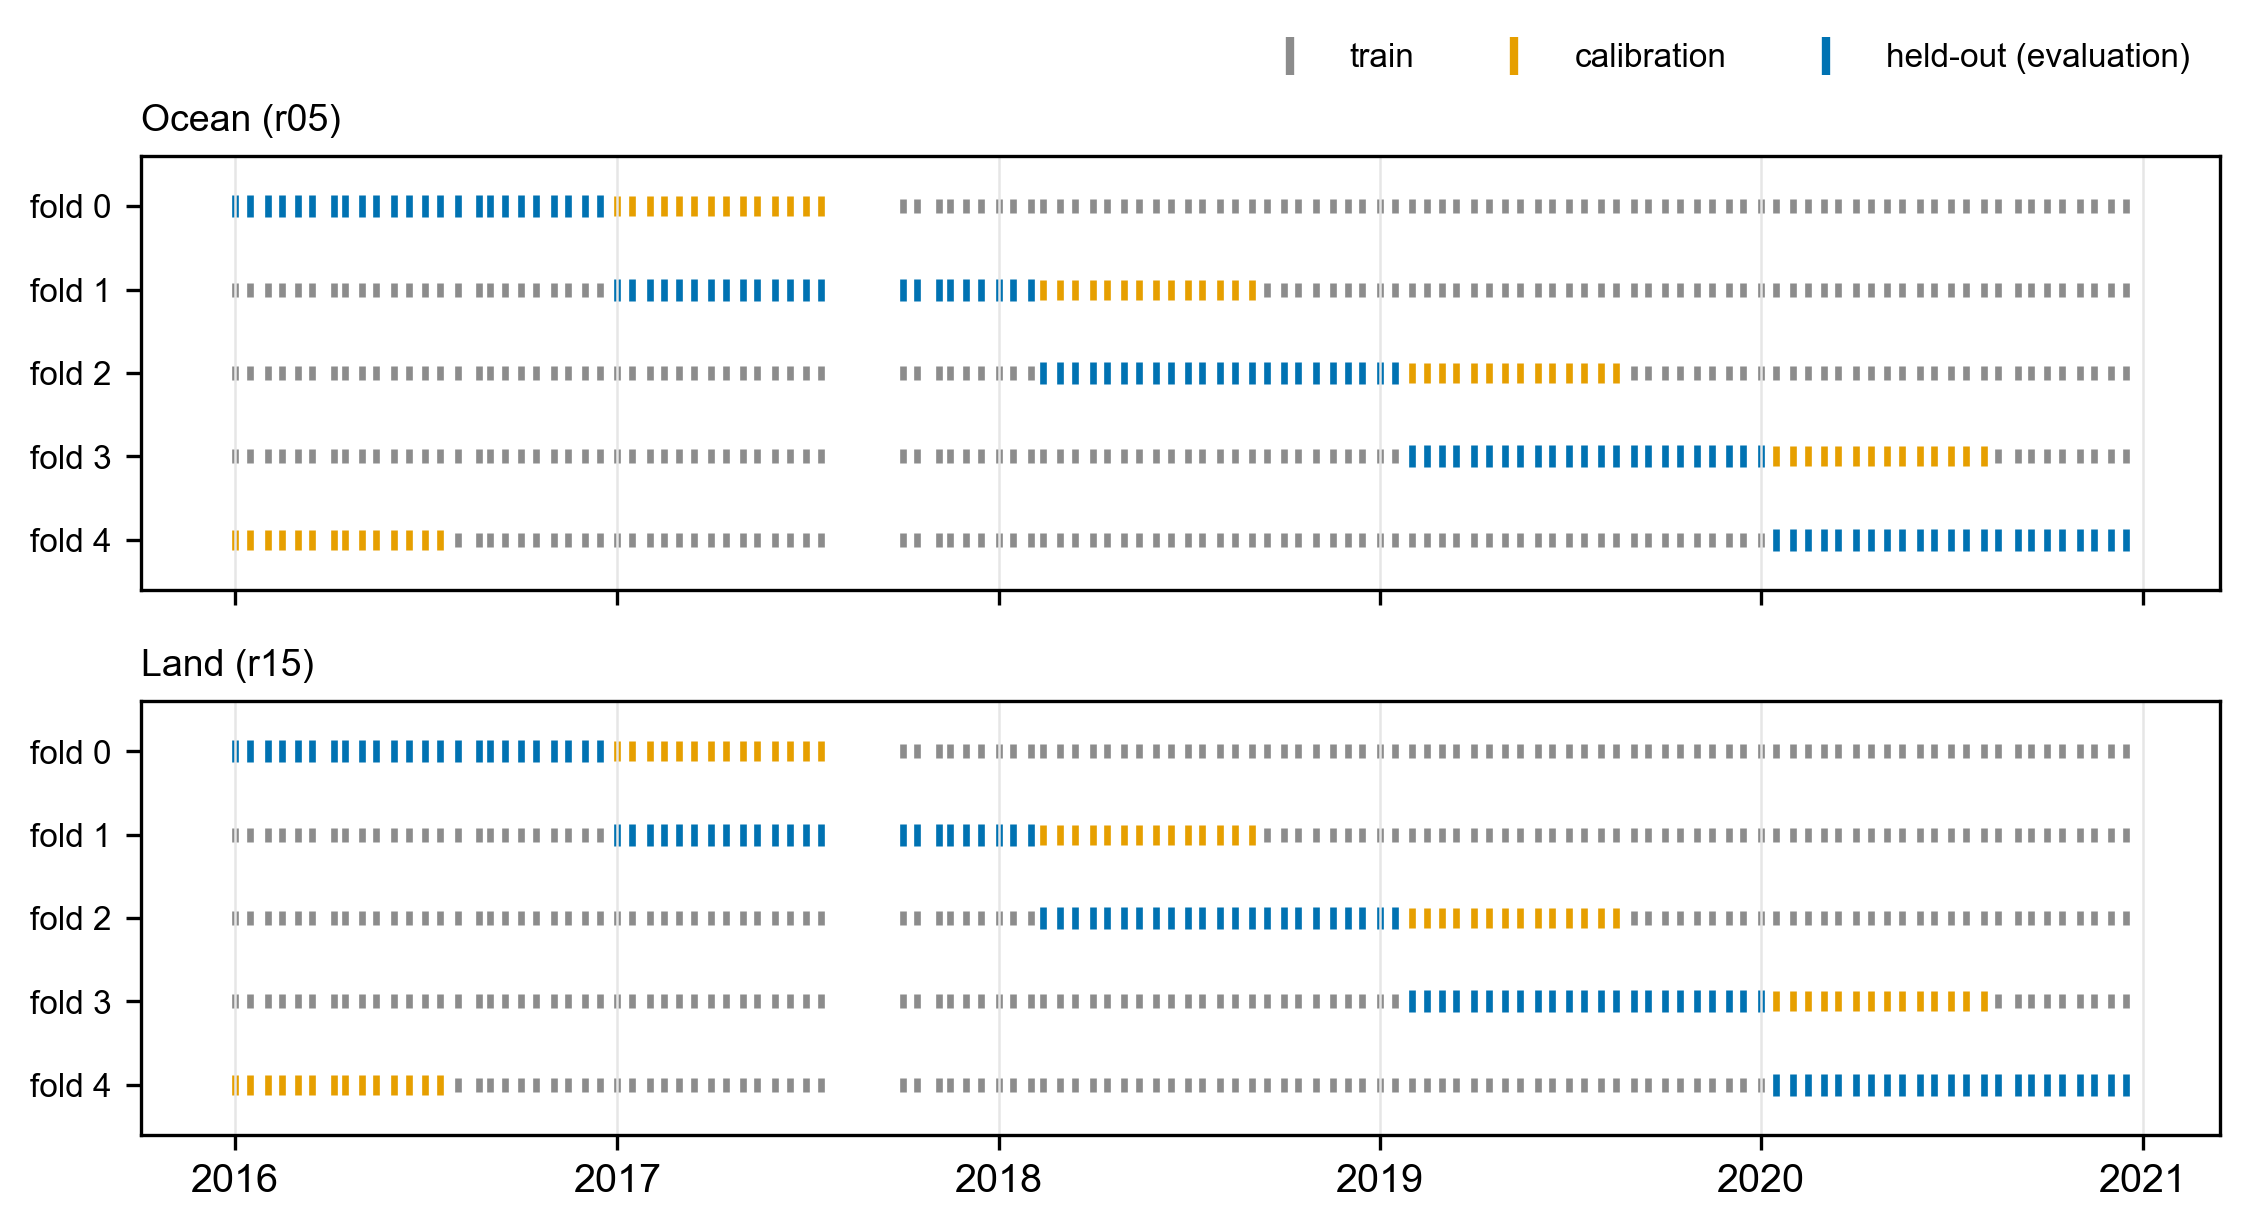
\includegraphics[width=\textwidth]{figures/figC2_fold_timeline.png}
\caption{Five-fold block-rotation cross-validation design over the 116
training and analysis dates. Each fold holds out one contiguous block of dates as
the test subset, and the remaining dates are divided into the proper-training and
the calibration subsets.}
\label{fig:5fold_illustration}
\end{figure}
%



\subsection{Model comparison}
\label{app:model_compare}



\begin{figure}[t]
\centering
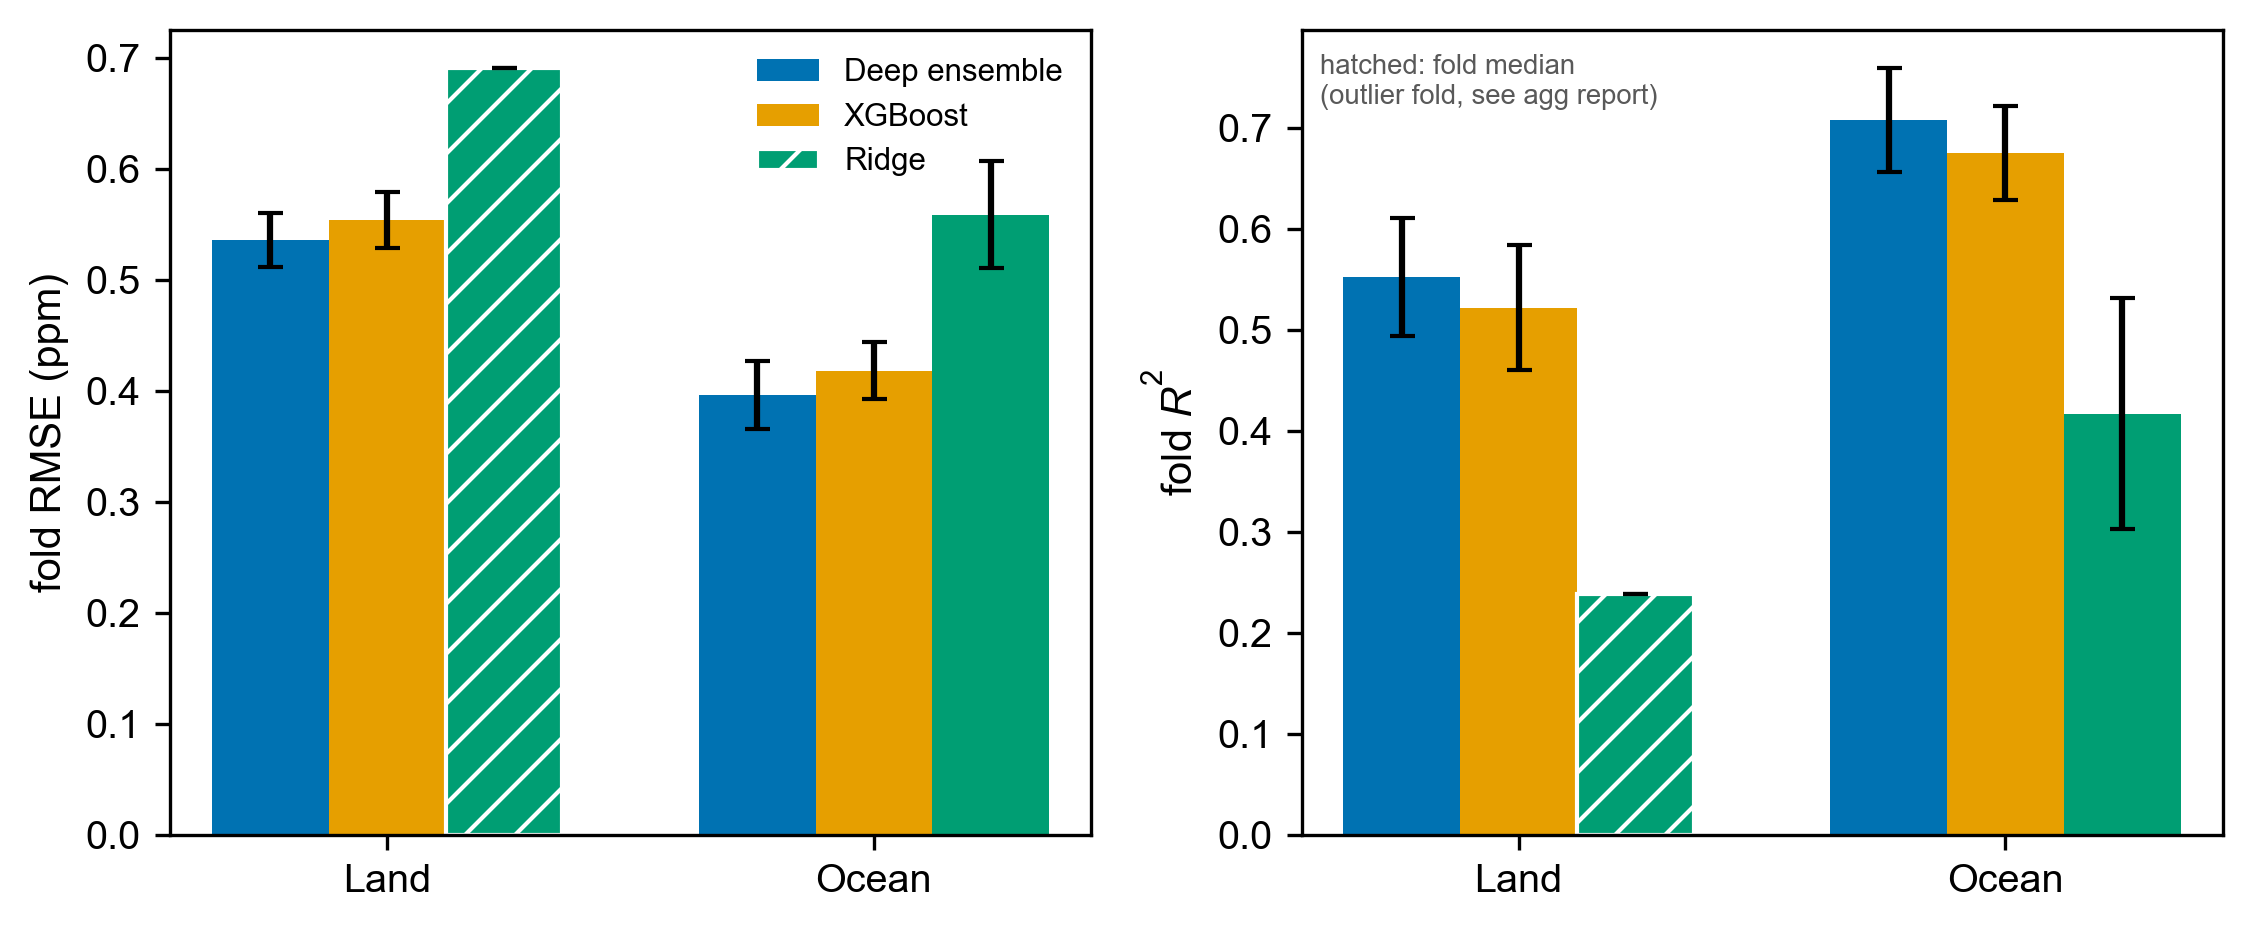
\includegraphics[width=0.8\textwidth]{figures/figC5_cv_model_comparison.png}
\caption{Date-blocked five-fold cross-validation of the anomaly target: held-out fold RMSE (left) and $R^2$ (right), mean ± std over folds, for the deep ensemble, XGBoost, and ridge baselines per surface. Ridge predictions pass the production output guard (Table C5 note).}
\label{fig:model_cv_compare}
\end{figure}



% Auto-generated by make_appendix_c_figures.py — do not hand-edit.
\begingroup\small
\begin{longtable}{lp{0.60\linewidth}}
\caption{Production training configuration of the per-surface deep ensembles, read from the ten fold run manifests (identical across surfaces and folds by assertion).}
\label{tab:training-config}\\
\tophline
Setting & Value \\
\middlehline
\endfirsthead
\multicolumn{2}{l}{\textit{(continued)}}\\
\tophline
Setting & Value \\
\middlehline
\endhead
\bottomhline
\endfoot
\bottomhline
\endlastfoot
Member architecture & MLP $n\rightarrow$64$\rightarrow$32$\rightarrow(\mu, \log\sigma^2)$ Gaussian heads \\
Normalization / dropout & layer normalization / 0.1 \\
Loss & $\beta$-NLL, $\beta = 1$ \\
Members per fold $M$ & 5 \\
Folds & 5, contiguous date blocks (Fig.~C2); pooled inference ensemble $5\times M = 25$ \\
Calibration split & 0.15 of training dates (date-blocked; early stopping and conformal calibration) \\
Optimizer & AdamW, lr 0.001, weight decay 0.0001 \\
Schedule & OneCycle (pct\_start 0.05, div 25, final div 1000) \\
Batch size / max epochs & 8192 / 500 (early stop, patience 50, best-validation checkpoint) \\
Gradient clip / seed & 1 / 42 \\
Feature set & \texttt{full} $+$ profile-EOF block (fold-fitted PCA) \\
Feature scaling & robust--standard scaler; log1p on AODs and footprint area; fitted on the training split only \\
Uncertainty calibration & split $+$ Mondrian conformal (cloud-distance bins), 90\,\% intervals \\
\end{longtable}
\endgroup


% Auto-generated by make_appendix_c_figures.py — do not hand-edit.
\begin{table}[t]
\caption{Fold-level sample sizes and held-out performance of the production deep ensemble. Dates: training/calibration/held-out date counts of the shared date-blocked fold structure (Fig.~C2); $n$: held-out soundings; RMSE (ppm) and $R^2$ against the anomaly target; cov$_{90}$ and width (ppm): empirical coverage and mean width of the Mondrian-conformal 90\,\% intervals.}
\label{tab:fold-sizes-metrics}
\small
\begin{tabular}{lcrrrrr}
\tophline
Fold & Dates (tr/cal/held) & $n$ & RMSE & $R^2$ & cov$_{90}$ & width \\
\middlehline
\multicolumn{7}{l}{\textit{Ocean (r05)}} \\
fold 0 & 78/14/24 & 1\,592\,441 & 0.449 & 0.619 & 0.945 & 1.74 \\
fold 1 & 79/14/23 & 1\,635\,886 & 0.397 & 0.710 & 0.945 & 1.53 \\
fold 2 & 79/14/23 & 1\,758\,400 & 0.375 & 0.747 & 0.955 & 1.57 \\
fold 3 & 79/14/23 & 1\,521\,313 & 0.380 & 0.727 & 0.956 & 1.57 \\
fold 4 & 79/14/23 & 1\,340\,722 & 0.381 & 0.735 & 0.978 & 1.90 \\
\middlehline
\multicolumn{7}{l}{\textit{Land (r15)}} \\
fold 0 & 78/14/24 & 803\,684 & 0.577 & 0.470 & 0.915 & 1.91 \\
fold 1 & 79/14/23 & 739\,808 & 0.537 & 0.577 & 0.898 & 1.68 \\
fold 2 & 79/14/23 & 755\,293 & 0.534 & 0.539 & 0.899 & 1.68 \\
fold 3 & 79/14/23 & 752\,939 & 0.519 & 0.628 & 0.908 & 1.70 \\
fold 4 & 79/14/23 & 792\,948 & 0.515 & 0.547 & 0.913 & 1.70 \\
\bottomhline
\end{tabular}
\end{table}


% Auto-generated by make_appendix_c_figures.py — do not hand-edit.
\begin{table*}[t]
\caption{Training-date manifests and evaluation-date disjointness. The 116 model dates (training, calibration, and held-out roles pooled over all five folds; identical for both surfaces) are compared against every independent evaluation set; the intersection column is computed from the per-run \texttt{training\_dates.json} manifests at table-generation time and enforced programmatically by the leakage guard in every evaluation builder.}
\label{tab:manifest-verification}
\small
\begin{tabular}{lrrcr}
\tophline
Set & Cases & Unique dates & Date range & $\cap$ model dates \\
\middlehline
Training $+$ calibration $+$ held (all folds) & — & 116 & 2016-01-01 -- 2020-12-15 & — \\
\middlehline
TCCON (A-train era) & 75 & 51 & 2014-12-03 -- 2021-12-29 & 0 \\
TCCON (drift era) & 21 & 21 & 2023-01-23 -- 2024-12-02 & 0 \\
ATom pseudo-columns & 8 & 8 & 2017-01-26 -- 2018-05-12 & 0 \\
Shipborne EM27/SUN & 4 & 4 & 2019-06-09 -- 2021-03-15 & 0 \\
\bottomhline
\end{tabular}
\end{table*}


% Auto-generated by make_appendix_c_figures.py — do not hand-edit.
\begin{table}[t]
\caption{Date-blocked five-fold cross-validation of the anomaly target: held-out fold RMSE (ppm) and $R^2$ (mean $\pm$ std over folds) for the deep ensemble (DE), XGBoost, and ridge baselines, per surface.}
\label{tab:cv-model-comparison}
\begin{tabular}{llrr}
\tophline
Surface & Model & RMSE (ppm) & $R^2$ \\
\middlehline
Ocean & DE & $0.396 \pm 0.027$ & $0.708 \pm 0.046$ \\
Ocean & XGBoost & $0.418 \pm 0.023$ & $0.675 \pm 0.042$ \\
Ocean & Ridge$^{*}$ & $0.537 \pm 0.023$ & $0.464 \pm 0.054$ \\
\middlehline
Land & DE & $0.536 \pm 0.022$ & $0.552 \pm 0.052$ \\
Land & XGBoost & $0.554 \pm 0.023$ & $0.522 \pm 0.055$ \\
Land & Ridge$^{*}$ & $0.673 \pm 0.021$ & $0.299 \pm 0.033$ \\
\bottomhline
\end{tabular}
\belowtable{$^{*}$Ridge predictions pass the production output guard (correction withheld where $|\mu| > 25$\,ppm), which the deployed chain applies to every model; it triggers on 18 of the $\sim$11.6\,M ridge held-out footprints — dominated by a single out-of-domain footprint whose unbounded linear extrapolation reaches $|\mu| \sim 10^{6}$\,ppm — and is not applied to the bounded DE/XGBoost outputs (max $|\mu| < 32$\,ppm).}
\end{table}


% Auto-generated by make_appendix_c_figures.py — do not hand-edit.
\begin{table}[t]
\caption{Fold-resolved held-out metrics (RMSE in ppm, $R^2$) for the deep ensemble, XGBoost, and ridge baselines under the shared date-blocked folds. Ridge values apply the production output guard of Table~C5.}
\label{tab:fold-resolved-baselines}
\small
\begin{tabular}{lrrrrrr}
\tophline
& \multicolumn{2}{c}{DE} & \multicolumn{2}{c}{XGBoost} & \multicolumn{2}{c}{Ridge} \\
Fold & RMSE & $R^2$ & RMSE & $R^2$ & RMSE & $R^2$ \\
\middlehline
\multicolumn{7}{l}{\textit{Ocean (r05)}} \\
fold 0 & 0.449 & 0.619 & 0.461 & 0.599 & 0.583 & 0.358 \\
fold 1 & 0.397 & 0.710 & 0.420 & 0.674 & 0.524 & 0.492 \\
fold 2 & 0.375 & 0.747 & 0.392 & 0.724 & 0.523 & 0.508 \\
fold 3 & 0.380 & 0.727 & 0.413 & 0.678 & 0.524$^{*}$ & 0.480 \\
fold 4 & 0.381 & 0.735 & 0.407 & 0.699 & 0.532 & 0.485 \\
\middlehline
\multicolumn{7}{l}{\textit{Land (r15)}} \\
fold 0 & 0.577 & 0.470 & 0.594 & 0.437 & 0.691 & 0.239 \\
fold 1 & 0.537 & 0.577 & 0.547 & 0.561 & 0.680 & 0.321 \\
fold 2 & 0.534 & 0.539 & 0.560 & 0.492 & 0.654$^{*}$ & 0.308 \\
fold 3 & 0.519 & 0.628 & 0.540 & 0.597 & 0.696$^{*}$ & 0.333 \\
fold 4 & 0.515 & 0.547 & 0.529 & 0.523 & 0.642 & 0.296 \\
\bottomhline
\end{tabular}
\belowtable{$^{*}$Folds where the guard withheld ridge corrections ($|\mu| > 25$\,ppm): ocean fold 3: 1; land fold 2: 1; land fold 3: 16 footprint(s). Unguarded, land fold 2 is dominated by a single out-of-domain footprint (raw $|\mu| \sim 10^{6}$\,ppm).}
\end{table}


% Auto-generated by make_appendix_c_figures.py — do not hand-edit.
\begin{table}[t]
\caption{Held-out date-blocked cross-validation of the feature-set ablation: fold mean $\pm$ std RMSE (ppm) and $R^2$ against the anomaly target for the production deep ensemble (full) and the variants retrained with one feature group removed (identical architecture, regularization, and folds). $\Delta$RMSE is the fold-mean change versus full. The TCCON-side ablation of the same variants is Table~2.}
\label{tab:cv-ablation}
\small
\begin{tabular}{lccr}
\tophline
Variant & RMSE & $R^2$ & $\Delta$RMSE \\
\middlehline
\multicolumn{4}{l}{\textit{Ocean (r05)}} \\
full & $0.396 \pm 0.027$ & $0.708 \pm 0.046$ & — \\
$-$spec & $0.408 \pm 0.027$ & $0.691 \pm 0.047$ & +0.011 \\
$-$contam & $0.431 \pm 0.025$ & $0.655 \pm 0.046$ & +0.035 \\
$-$xco2 & $0.460 \pm 0.005$ & $0.608 \pm 0.007$ & +0.064 \\
$-$xco2$-$spec & $0.523 \pm 0.004$ & $0.495 \pm 0.004$ & +0.126 \\
$-$xco2$-$contam & $0.502 \pm 0.005$ & $0.535 \pm 0.010$ & +0.105 \\
\middlehline
\multicolumn{4}{l}{\textit{Land (r15)}} \\
full & $0.536 \pm 0.022$ & $0.552 \pm 0.052$ & — \\
$-$spec & $0.542 \pm 0.016$ & $0.543 \pm 0.044$ & +0.006 \\
$-$contam & $0.579 \pm 0.020$ & $0.478 \pm 0.062$ & +0.042 \\
$-$xco2 & $0.598 \pm 0.015$ & $0.444 \pm 0.057$ & +0.061 \\
$-$xco2$-$spec & $0.637 \pm 0.011$ & $0.369 \pm 0.050$ & +0.101 \\
$-$xco2$-$contam & $0.666 \pm 0.014$ & $0.311 \pm 0.066$ & +0.129 \\
\bottomhline
\end{tabular}
\belowtable{Land fold 4 of the $-$contam and $-$xco2$-$contam variants carries the pre-regularization checkpoint (a healthy fold in both trainings; see the 2026-07-17 ablation report).}
\end{table}


% Generated by manuscript/scripts/make_manuscript_tables.py — do not hand-edit.
% Requires booktabs. Define in the preamble:
%   \newcommand{\xcobc}{$X_{\mathrm{CO2}}^{\mathrm{bc}}$}
%   \newcommand{\xcoraw}{$X_{\mathrm{CO2}}^{\mathrm{raw}}$}
\begin{table}[htbp]
\centering
\caption{Four XCO$_2$ series against TCCON (ppm; AK-harmonized, 100\,km / $\pm$60\,min): pre-bias-correction \xcoraw{} (raw), operationally bias-corrected \xcobc{} (bc), the production ML correction applied to \xcobc{} (ML(bc)), and an ML correction trained on and applied to \xcoraw{} directly (ML(raw)). Best of the three corrected/operational series per slice in bold. Cloud-distance slices split each surface at its production target radius (ocean 5\,km, land 15\,km; Sect.~3.1). ML(raw) reaching within $\sim$0.1\,ppm of the production chain shows the per-footprint ML layer can absorb most of the operational bias correction over these scenes.}
\label{tab:raw-bc-ml}
\small
\begin{tabular}{lrrrrrrrr}
\specialrule{1.2pt}{0pt}{2pt}
Slice & \multicolumn{4}{c}{fp-RMSE} & \multicolumn{4}{c}{Bias} \\
\cmidrule(lr){2-5}\cmidrule(lr){6-9}
 & raw & bc & ML(bc) & ML(raw) & raw & bc & ML(bc) & ML(raw) \\
\midrule
Pooled, QF 0+1 & 2.96 & 3.29 & 1.22 & \textbf{1.18} & -0.55 & -0.71 & -0.36 & -0.16 \\
Pooled, QF$\,$=$\,$0 & 1.47 & 1.01 & \textbf{0.83} & 0.99 & +0.15 & +0.08 & -0.20 & -0.16 \\
Pooled, QF$\,$=$\,$1 & 4.04 & 4.68 & 1.54 & \textbf{1.37} & -0.92 & -1.01 & -0.40 & -0.18 \\
Ocean & 1.83 & 1.27 & \textbf{0.98} & 1.55 & -0.04 & -0.02 & +0.12 & +0.12 \\
Ocean, QF$\,$=$\,$1 & 2.31 & 1.76 & \textbf{1.25} & 1.81 & -0.31 & -0.11 & +0.14 & +0.11 \\
Ocean $\leq$5\,km & 2.12 & 1.54 & \textbf{1.12} & 1.72 & -0.13 & -0.12 & +0.10 & +0.12 \\
Ocean $\leq$5\,km, QF$\,$=$\,$1 & 2.52 & 1.92 & \textbf{1.29} & 1.89 & -0.33 & -0.20 & +0.12 & +0.12 \\
Ocean $\geq$5\,km & 1.58 & 1.02 & \textbf{0.86} & 1.42 & -0.25 & -0.05 & +0.02 & -0.14 \\
Land & 3.02 & 3.38 & 1.23 & \textbf{1.15} & -0.82 & -1.15 & -0.49 & -0.18 \\
Land, QF$\,$=$\,$1 & 4.08 & 4.75 & 1.55 & \textbf{1.35} & -1.21 & -1.45 & -0.55 & -0.22 \\
Land $\leq$15\,km & 3.26 & 3.71 & 1.31 & \textbf{1.22} & -0.85 & -1.20 & -0.52 & -0.19 \\
Land $\leq$15\,km, QF$\,$=$\,$1 & 4.20 & 4.94 & 1.59 & \textbf{1.38} & -1.32 & -1.56 & -0.60 & -0.25 \\
Land $\geq$15\,km & 1.59 & 0.95 & \textbf{0.79} & 0.81 & -0.28 & -0.32 & -0.42 & -0.42 \\
\specialrule{1.2pt}{2pt}{0pt}
\end{tabular}
\end{table}





Include:

- full feature dictionary with units, transformations, and source products;
- land and ocean architecture, beta-NLL definition, regularization, optimizer,
  learning-rate schedule, early stopping, and seeds;
- fold construction, calibration split, scaler and fold-PCA fitting rules;
- ensemble aggregation and predictive-variance decomposition;
- Mondrian conformal procedure and cloud-distance-dependent inflation, where
  applicable;
- leakage-guard logic and the verified training/evaluation date intersection;
- model and feature-set production tags.

Planned items:

- **Fig. C1:** training and evaluation data-flow diagram;
- **Fig. C2:** fold timeline showing contiguous date blocks;
- **Table C1:** full predictor inventory;
- **Table C2:** hyperparameters and training configuration;
- **Table C3:** fold-level sample sizes and performance;
- **Table C4:** training manifests and zero-overlap verification.

Keep the main text to predictor groups and essential architecture. Individual
features and hyperparameters belong here.

\section{Cross-validation, baselines, and feature attribution}
\label{app:evaluation}




\subsection{Averaging-kernel and Prior Harmonization Operation}
\label{app:ak_operation}
For the valid OCO-2 soundings \(s\in\mathcal S\) collocated with a TCCON station, the case-level mean observation operator is



\begin{equation}
    \bar{h}_j = \frac{1}{N_{\mathrm{OCO}}}
             \sum_{s\in\mathcal{S}} h_{s,j}, \\
\end{equation}

\begin{equation}
    \bar{A}_j = \frac{1}{N_{\mathrm{OCO}}}
             \sum_{s\in\mathcal{S}} A_{s,j}, \\
\end{equation}

\begin{equation}
    \bar{x}_{a,j}^{\mathrm{OCO}} =
             \frac{1}{N_{\mathrm{OCO}}}
             \sum_{s\in\mathcal{S}} x_{a,s,j}^{\mathrm{OCO}}, \\
\end{equation}

\begin{equation}
    \bar{p}_j^{\mathrm{OCO}} =
             \frac{1}{N_{\mathrm{OCO}}}
             \sum_{s\in\mathcal{S}} p_{s,j}^{\mathrm{OCO}}, \\
\end{equation}

\begin{equation}
    \bar{X}_{a}^{\mathrm{OCO}} =
             \frac{1}{N_{\mathrm{OCO}}}
             \sum_{s\in\mathcal{S}} X_{a,s}^{\mathrm{OCO}},
\end{equation}




where \(h_j\) is the pressure-weighting function, \(A_j\) is the normalized column averaging kernel, ($x_{a,j}^{\mathrm{OCO}}$) is the OCO-2 prior profile, and ($X_a^{\mathrm{OCO}}$) is prior ($\mathrm{X_{CO2}}$).



For each TCCON observation \(i\), its prior profile is scaled by the retrieved column ratio:

\begin{equation}
\gamma_i =
\frac{X_{\mathrm{CO_2},i}^{\mathrm{TCCON}}}
     {X_{a,i}^{\mathrm{TCCON}}},
\qquad
x_i^{\mathrm{TCCON}}(p)
=
\gamma_i\,x_{a,i}^{\mathrm{TCCON}}(p).
\end{equation}


The scaled profile is interpolated linearly in log-pressure onto the mean OCO-2 pressure grid:

\begin{equation}
\tilde{x}_{i,j}^{\mathrm{TCCON}}
=
\mathcal{I}_{\ln p}
\left[
x_i^{\mathrm{TCCON}}(p)
\right]
\left(\bar{p}_j^{\mathrm{OCO}}\right).
\end{equation}


The TCCON profile as it would be observed by OCO-2 is then

\begin{equation}
\widehat{X}_{\mathrm{CO_2},i}^{\mathrm{TCCON}\rightarrow\mathrm{OCO}}
=
\bar{X}_{a}^{\mathrm{OCO}}
+
\sum_{j=1}^{N_{\mathrm{lev}}}
\bar{h}_j\,\bar{A}_j
\left(
\tilde{x}_{i,j}^{\mathrm{TCCON}}
-
\bar{x}_{a,j}^{\mathrm{OCO}}
\right),
\end{equation}

with \(N_{\mathrm{lev}}=20\) for the OCO-2 Lite product.

Finally, the harmonized case reference is

\begin{equation}
\overline{X}_{\mathrm{CO_2}}^{\mathrm{TCCON}\rightarrow\mathrm{OCO}}
=
\frac{1}{N_{\mathrm{TCCON}}}
\sum_{i=1}^{N_{\mathrm{TCCON}}}
\widehat{X}_{\mathrm{CO_2},i}^{\mathrm{TCCON}\rightarrow\mathrm{OCO}},
\end{equation}

and the reported averaging-kernel/prior adjustment is

\begin{equation}
\Delta_{\mathrm{AK}}
=
\overline{X}_{\mathrm{CO_2}}^{\mathrm{TCCON}\rightarrow\mathrm{OCO}}
-
\overline{X}_{\mathrm{CO_2}}^{\mathrm{TCCON}}.
\end{equation}


The code reports the population standard deviation:

\begin{equation}
\sigma_{\mathrm{AK}}
=
\left[
\frac{1}{N_{\mathrm{TCCON}}}
\sum_{i=1}^{N_{\mathrm{TCCON}}}
\left(
\widehat{X}_{\mathrm{CO_2},i}^{\mathrm{TCCON}\rightarrow\mathrm{OCO}}
-
\overline{X}_{\mathrm{CO_2}}^{\mathrm{TCCON}\rightarrow\mathrm{OCO}}
\right)^2
\right]^{1/2}.
\end{equation}

% ---------------------------------------------------------------------------
% Table -- TCCON stations used
% ---------------------------------------------------------------------------
\begin{table}[htbp]
\centering
\caption{TCCON GGG2020 stations used in the validation set. Coordinates are from the public TCCON site metadata pages. The near-ocean flag is a qualitative coastal, island, or near-coast classification for interpreting validation geography; it is not a GIS-derived coastline-distance metric.} 
\label{tab:tccon-stations-used}
\small
\begin{tabularx}{\textwidth}{llrrcX}
\specialrule{1.2pt}{0pt}{2pt}
Code & Site & Longitude & Latitude & Near ocean & Reference \\
\midrule
bu & burgos01 & 120.6496 & 18.5325 & Yes & \citep{tccon-bu-dataref,tccon-bu-siteref} \\
ci & pasadena01 & -118.1270 & 34.1360 & Yes & \citep{tccon-ci-dataref} \\
db & darwin01 & 130.9266 & -12.4559 & Yes & \citep{tccon-db-dataref,tccon-db-siteref} \\
df & edwards01 & -117.8811 & 34.9599 & No & \citep{tccon-df-dataref} \\
et & easttroutlake01 & -104.9867 & 54.3537 & No & \citep{tccon-et-dataref} \\
iz & izana01 & -16.5000 & 28.3000 & Yes & \citep{tccon-iz-dataref} \\
js & saga01 & 130.2882 & 33.2410 & Yes & \citep{tccon-js-dataref,tccon-js-siteref} \\
ka & karlsruhe01 & 8.4380 & 49.1000 & No & \citep{tccon-ka-dataref} \\
ma & manaus01 & -60.5983 & -3.2133 & No & \citep{tccon-ma-dataref,tccon-ma-siteref} \\
ny & nyalesund01 & 11.9230 & 78.9230 & Yes & \citep{tccon-ny-dataref} \\
oc & lamont01 & -97.4860 & 36.6040 & No & \citep{tccon-oc-dataref} \\
or & orleans01 & 2.1130 & 47.9700 & No & \citep{tccon-or-dataref} \\
pa & parkfalls01 & -90.2730 & 45.9450 & No & \citep{tccon-pa-dataref,tccon-pa-siteref} \\
pr & paris01 & 2.3560 & 48.8460 & No & \citep{tccon-pr-dataref} \\
ra & reunion01 & 55.4850 & -20.9010 & Yes & \citep{tccon-ra-dataref} \\
rj & rikubetsu01 & 143.7700 & 43.4600 & No & \citep{tccon-rj-dataref} \\
wg & wollongong01 & 150.8798 & -34.4060 & Yes & \citep{tccon-wg-dataref} \\
xh & xianghe01 & 116.9600 & 39.7500 & No & \citep{tccon-xh-dataref,tccon-xh-siteref} \\
\specialrule{1.2pt}{2pt}{0pt}
\end{tabularx}
\end{table}


% ---------------------------------------------------------------------------
% Table -- training / analysis dates
% ---------------------------------------------------------------------------
\begin{table}[t]
\centering
\caption{Dates of the 2016--2020 training and analysis set. Entries give the
day of month sampled in each month; the nominal sampling is the 1st and the
15th of every month, and a neighbouring day is substituted where the nominal
date has no usable OCO-2 or MODIS granule. A dash marks a month with no
available data. The set contains 116 dates in total.}
\label{tab:dates_training}
\setlength{\tabcolsep}{3.2pt}
\footnotesize
\begin{tabular}{@{}lcccccccccccc@{}}
\toprule
Year & Jan & Feb & Mar & Apr & May & Jun & Jul & Aug & Sep & Oct & Nov & Dec \\
\midrule
2016 & 1, 15 & 1, 15 & 1, 15 & 5, 15 & 1, 15 & 1, 15 & 1, 15 & 1, 21 & 1, 15 & 1, 15 & 1, 15 & 1, 15 \\
2017 & 1, 15 & 1, 15 & 1, 15 & 1, 15 & 1, 15 & 1, 15 & 1, 15 & -- & -- & 1, 15 & 5, 15 & 1, 15 \\
2018 & 1, 15 & 1, 12 & 1, 15 & 1, 15 & 1, 15 & 1, 15 & 1, 15 & 1, 15 & 1, 15 & 1, 15 & 1, 17 & 1, 15 \\
2019 & 1, 15 & 1, 15 & 1, 15 & 1, 15 & 1, 15 & 1, 15 & 1, 15 & 1, 15 & 1, 15 & 1, 15 & 1, 15 & 1, 15 \\
2020 & 1, 15 & 1, 15 & 1, 15 & 1, 15 & 1, 15 & 1, 15 & 1, 15 & 1, 15 & 3, 15 & 1, 15 & 1, 15 & 1, 15 \\
\bottomrule
\end{tabular}
\end{table}

% ---------------------------------------------------------------------------
% Table -- observation comparison set
% ---------------------------------------------------------------------------
\begin{longtable}{@{}llcp{0.52\textwidth}@{}}
\caption{Dates of the observation-comparison set, by validation reference. The
TCCON cases are separated into the A-Train period, during which Aqua and OCO-2
flew in formation, and the free-drift period after Aqua left the A-Train in
2022, for which the MODIS collocation window is widened
(Sect.~\ref{sec:method-cld_dist_xco2_anom}). One case is one station--day.
None of the 82 distinct comparison dates appears in the training and analysis
set of Table~\ref{tab:dates_training}.}
\label{tab:dates_comparison}\\
\toprule
Reference & Code & $N$ & Dates \\
\midrule
\endfirsthead
\toprule
Reference & Code & $N$ & Dates \\
\midrule
\endhead
\midrule \multicolumn{4}{r}{\emph{continued on next page}} \\
\endfoot
\bottomrule
\endlastfoot

\multicolumn{4}{@{}l}{\textbf{TCCON, A-Train period (2014--2021)} --- 75 cases, 18 stations} \\
Burgos          & \texttt{bu} & 2  & 2018-10-24, 2020-03-30 \\
Caltech         & \texttt{ci} & 1  & 2018-06-03 \\
Darwin          & \texttt{db} & 3  & 2015-06-05, 2015-08-01, 2021-06-21 \\
East Trout Lake & \texttt{et} & 4  & 2017-02-06, 2018-06-03, 2021-05-26, 2021-09-06 \\
Edwards         & \texttt{df} & 7  & 2015-07-06, 2015-07-15, 2017-02-03, 2019-07-10, 2021-02-10, 2021-09-06, 2021-09-26 \\
Iza\~{n}a       & \texttt{iz} & 3  & 2019-03-13, 2019-07-10, 2020-04-05 \\
Karlsruhe       & \texttt{ka} & 2  & 2018-10-10, 2019-07-30 \\
Lamont          & \texttt{oc} & 3  & 2018-06-03, 2021-04-24, 2021-12-29 \\
Manaus          & \texttt{ma} & 3  & 2014-12-03, 2015-03-23, 2015-07-06 \\
Ny-\AA{}lesund  & \texttt{ny} & 10 & 2015-06-05, 2015-07-15, 2016-09-10, 2017-05-25, 2017-06-17, 2019-06-09, 2020-07-11, 2020-07-26, 2021-07-03, 2021-09-08 \\
Orl\'{e}ans     & \texttt{or} & 2  & 2015-07-15, 2018-08-17 \\
Paris           & \texttt{pr} & 3  & 2015-07-15, 2018-08-17, 2020-09-16 \\
Park Falls      & \texttt{pa} & 2  & 2016-11-05, 2021-10-16 \\
R\'{e}union     & \texttt{ra} & 14 & 2015-03-17, 2015-05-18, 2015-05-20, 2015-07-14, 2015-07-23, 2015-08-01, 2016-09-11, 2016-11-05, 2017-03-22, 2017-04-23, 2017-05-16, 2017-05-25, 2020-03-30, 2020-07-11 \\
Rikubetsu       & \texttt{rj} & 1  & 2020-03-30 \\
Saga            & \texttt{js} & 6  & 2017-02-03, 2018-09-02, 2019-03-13, 2020-10-05, 2021-03-18, 2021-09-26 \\
Wollongong      & \texttt{wg} & 7  & 2018-08-17, 2019-07-30, 2019-09-14, 2020-09-16, 2020-12-23, 2021-03-29, 2021-07-03 \\
Xianghe         & \texttt{xh} & 2  & 2019-06-09, 2020-02-11 \\
\addlinespace

\multicolumn{4}{@{}l}{\textbf{TCCON, Aqua free-drift period (2023--2024)} --- 21 cases, 7 stations} \\
Burgos          & \texttt{bu} & 3  & 2023-01-23, 2023-02-10, 2023-03-23 \\
East Trout Lake & \texttt{et} & 1  & 2024-06-26 \\
Edwards         & \texttt{df} & 1  & 2023-06-26 \\
Karlsruhe       & \texttt{ka} & 3  & 2023-04-04, 2023-08-10, 2023-09-11 \\
Park Falls      & \texttt{pa} & 2  & 2023-03-19, 2024-03-10 \\
Wollongong      & \texttt{wg} & 10 & 2023-01-28, 2023-04-25, 2023-05-06, 2023-05-20, 2024-04-22, 2024-07-27, 2024-08-03, 2024-09-20, 2024-11-23, 2024-12-02 \\
Xianghe         & \texttt{xh} & 1  & 2023-08-14 \\
\addlinespace

\multicolumn{4}{@{}l}{\textbf{ATom airborne campaign} --- 8 dates, 17 vertical profile legs} \\
ATom-1 (Pacific)   & \texttt{atom} & 4 & 2017-01-26 (2), 2017-02-04 (2), 2017-02-06 (3), 2017-02-10 (1) \\
ATom-3 (Pacific)   & \texttt{atom} & 3 & 2017-10-09 (2), 2017-10-20 (4), 2017-10-27 (1) \\
ATom-4             & \texttt{atom} & 1 & 2018-05-12 (2) \\
\addlinespace

\multicolumn{4}{@{}l}{\textbf{Shipborne campaigns} --- 4 dates, 2 cruises} \\
SONNE SO268     & \texttt{so268}  & 3 & 2019-06-09, 2019-06-14, 2019-06-22 \\
Mirai MR21-01   & \texttt{mr2101} & 1 & 2021-03-15 \\

\end{longtable}


\section{Null tests, negative controls, and failure cases}
\label{app:more_tccon_test}




\subsection{Null tests}
\label{app:null-test}


\begin{figure}[t]
\centering
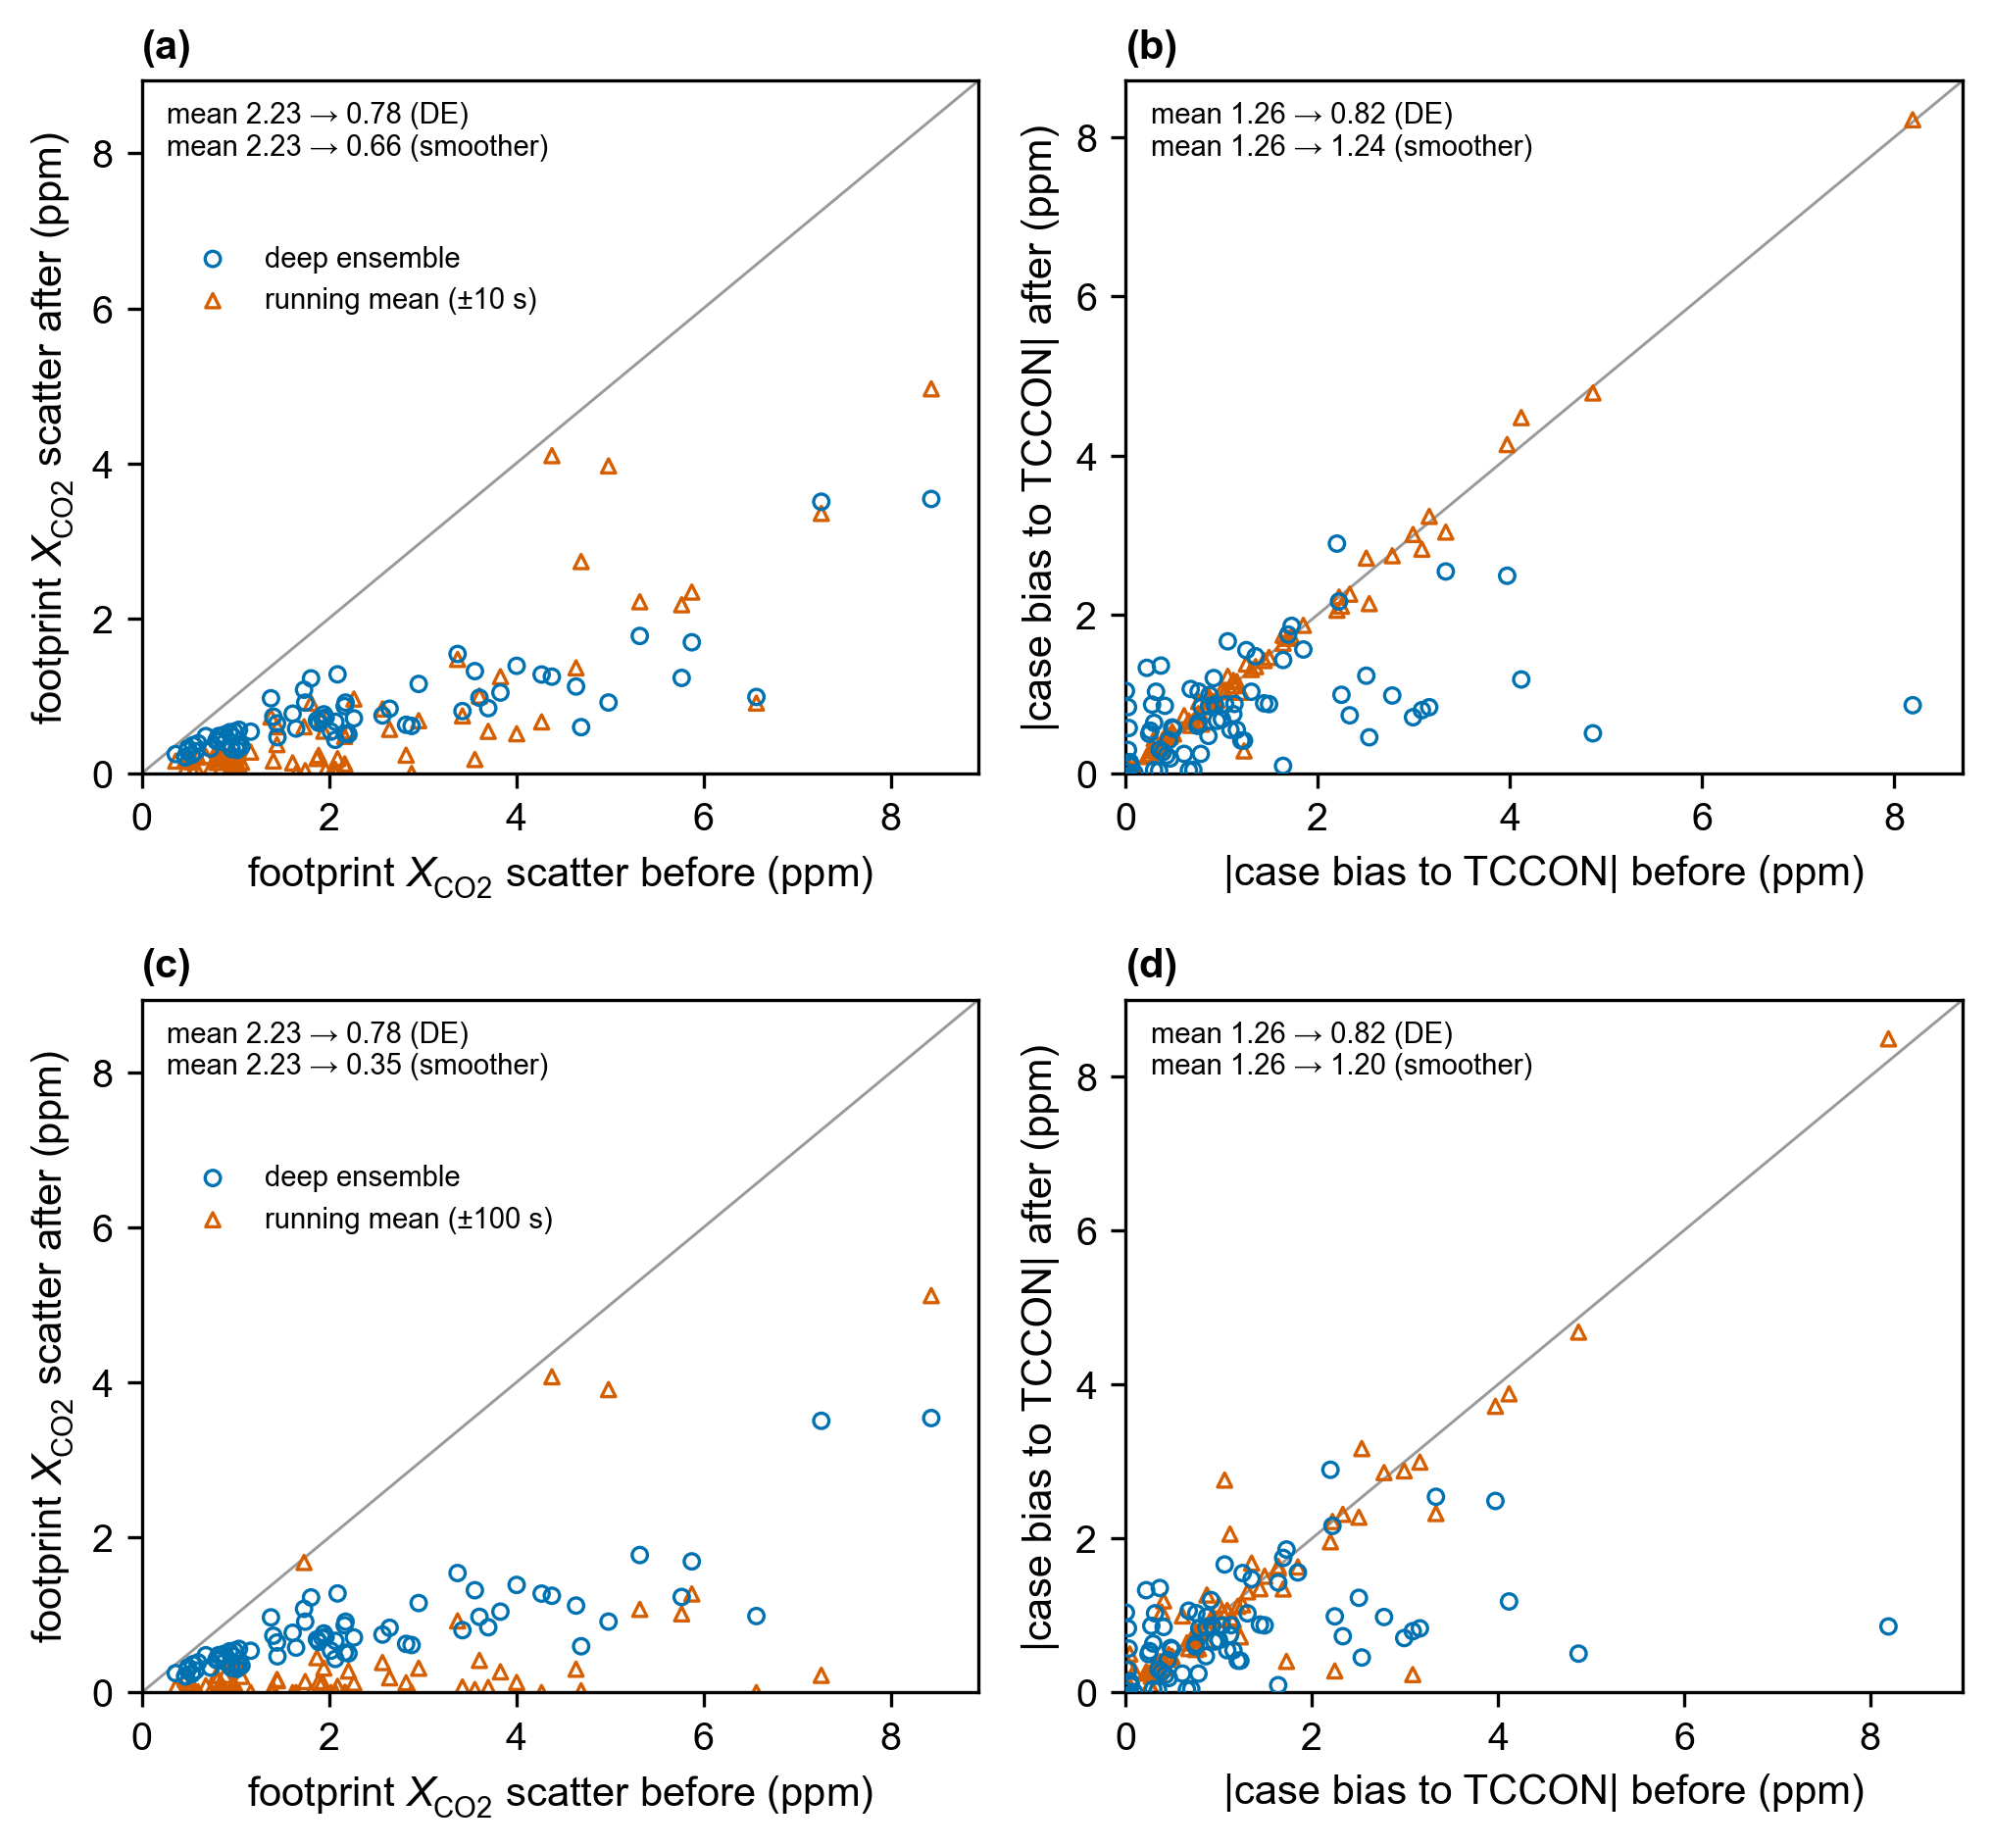
\includegraphics[width=0.8\textwidth]{figures/figE1_smoother_windows.png}
\caption{Feature-free smoother null: footprint-scatter collapse and TCCON station-day bias for orbit-local running-mean smoothers of half-width $\pm$10, $\pm$30, and $\pm$100 s beside the deep ensemble, under identical footprints, guards, and TCCON chain (windows not shown in main-text Fig.~\ref{fig:smoother_null}).}
\label{app-fig:smoother_null_full}
\end{figure}



\subsection{Negative controls}
\label{app:neg-control}



\begin{figure}[t]
\centering
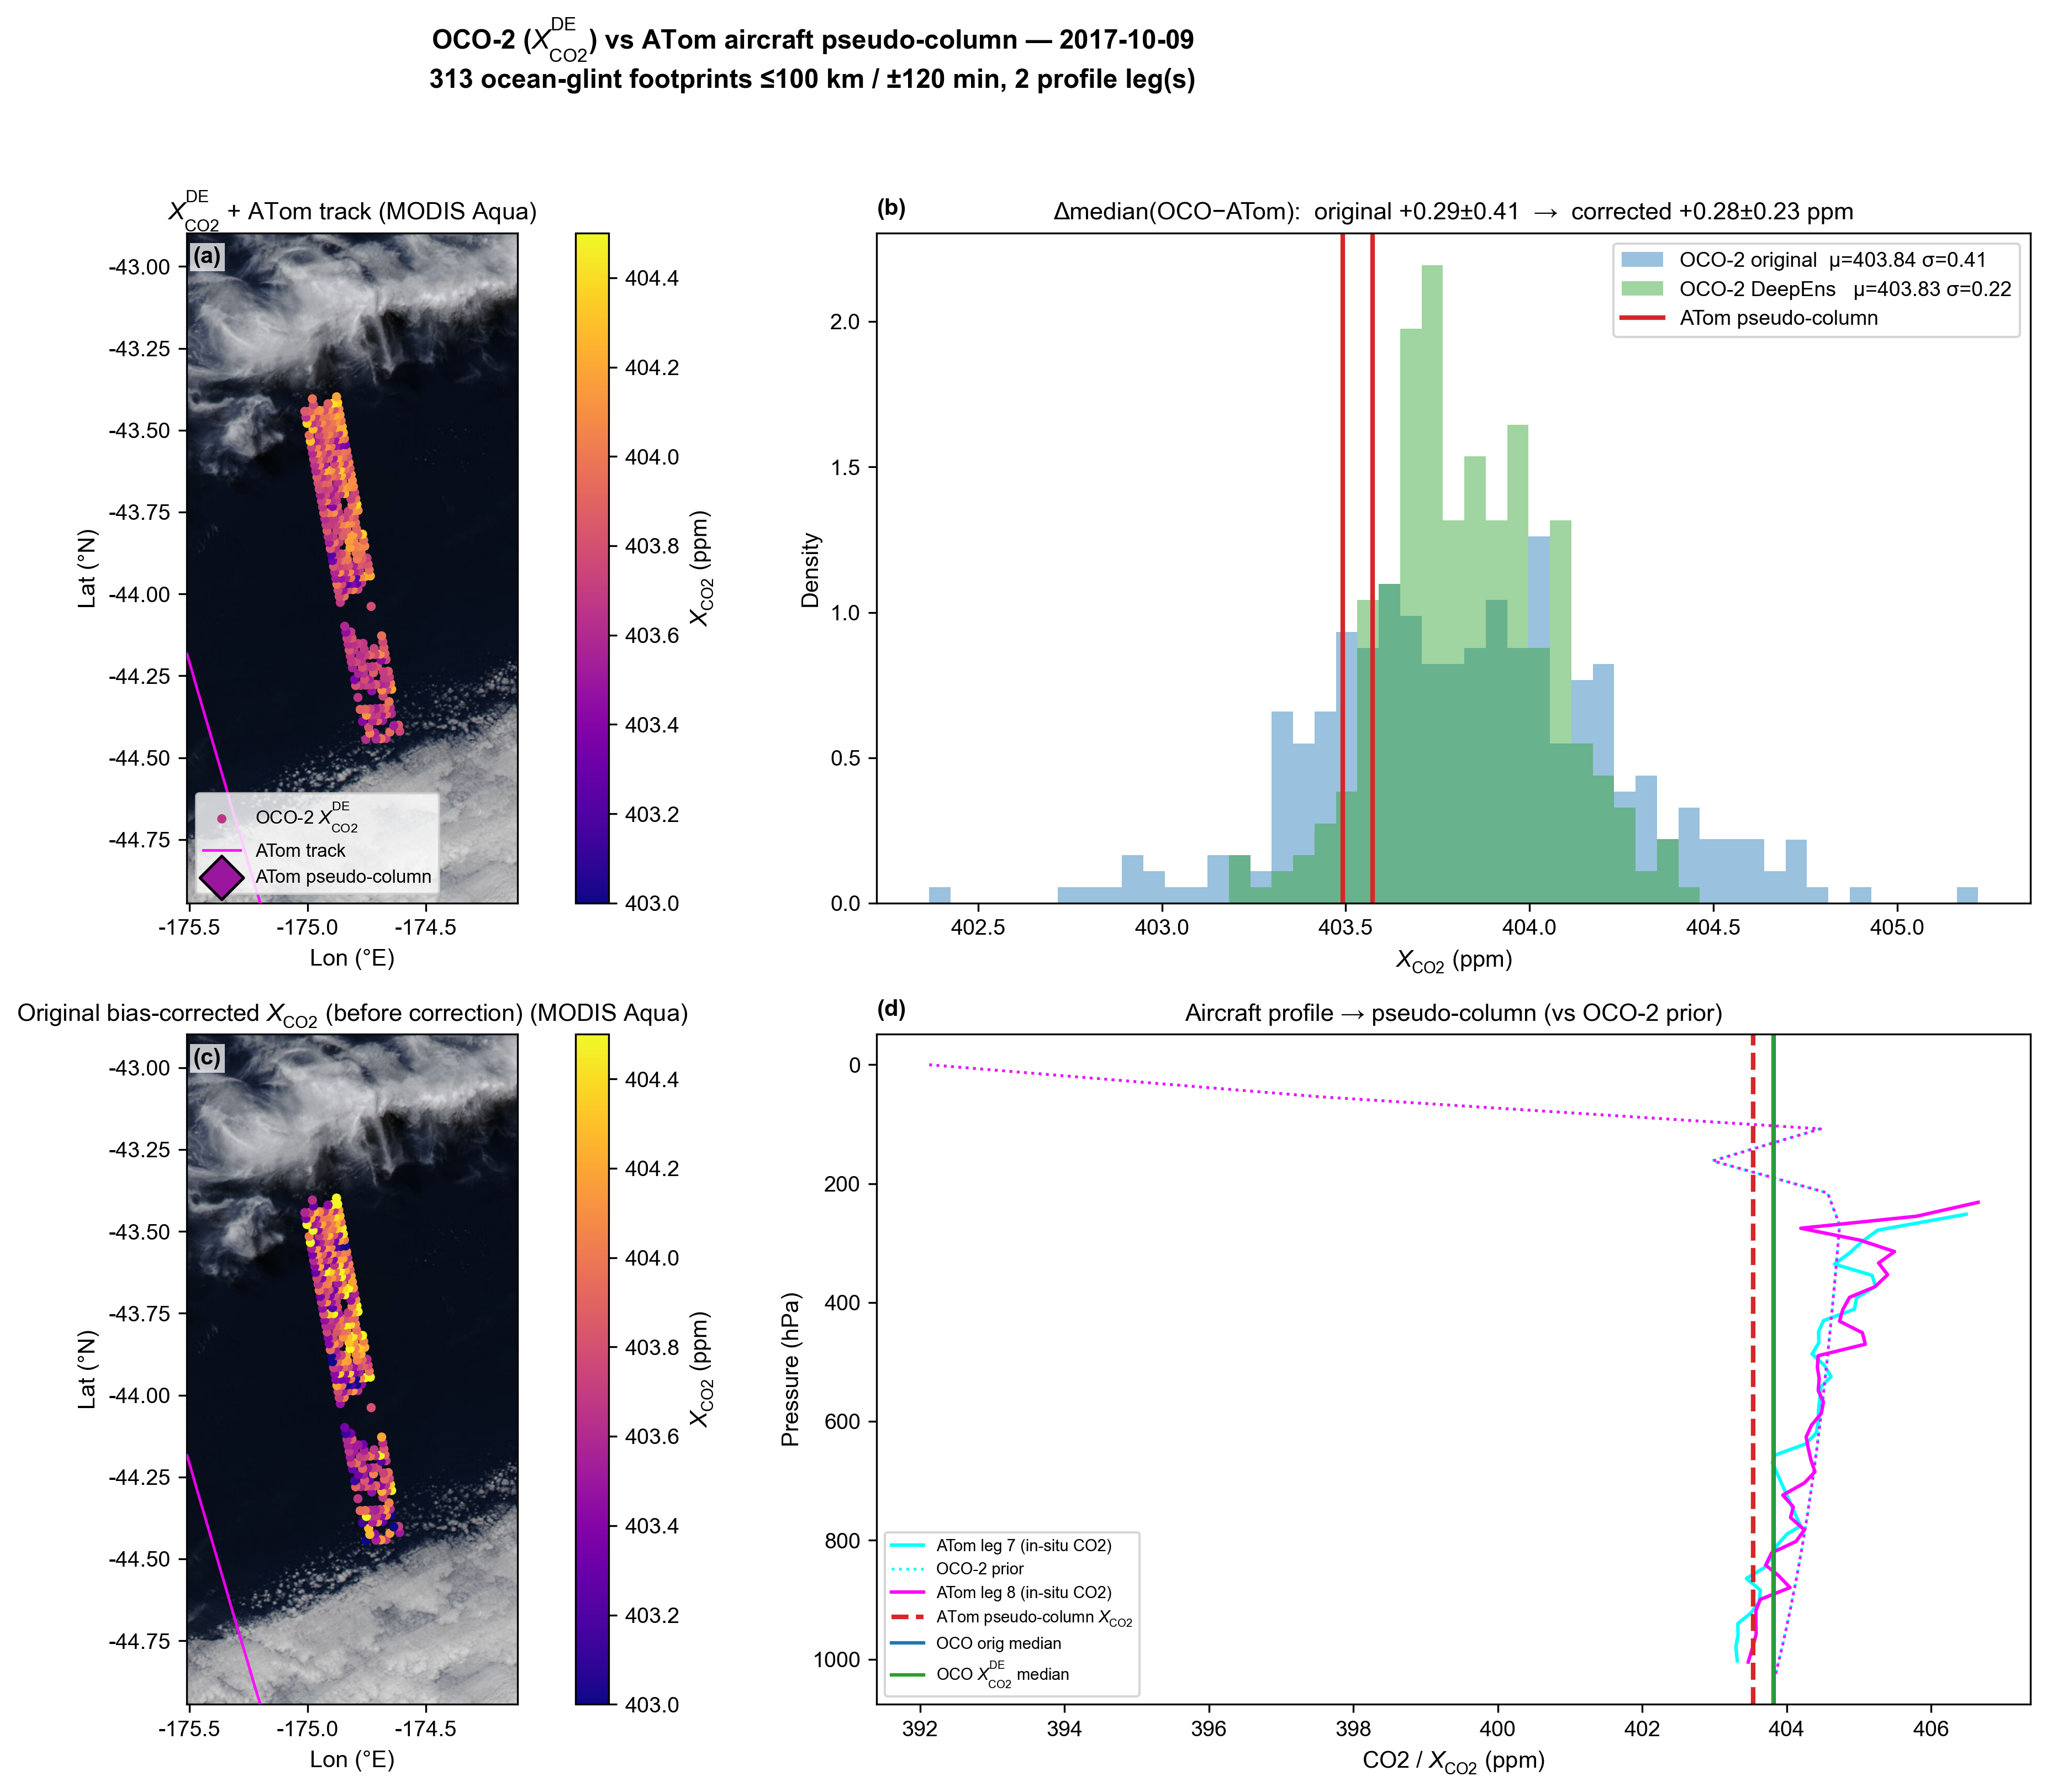
\includegraphics[width=0.8\textwidth]{figures/figE2_atom_farcloud_control.png}
\caption{ATom far-cloud negative control, 9 October 2017 (313 ocean-glint footprints within 100 km / ±120 min of two profile legs; median nearest-cloud distance 18 km): corrected and original \xco maps over the coincident MODIS Aqua true-colour scene (local day 8 October 2017 — the overpass crosses the antimeridian, where the imagery date is the local day) with the flight track, footprint distributions against the ATom pseudo-column, and the aircraft profiles with the OCO-2 prior.}
\label{app-fig:atom_far_cld}
\end{figure}


\begin{figure}[t]
\centering
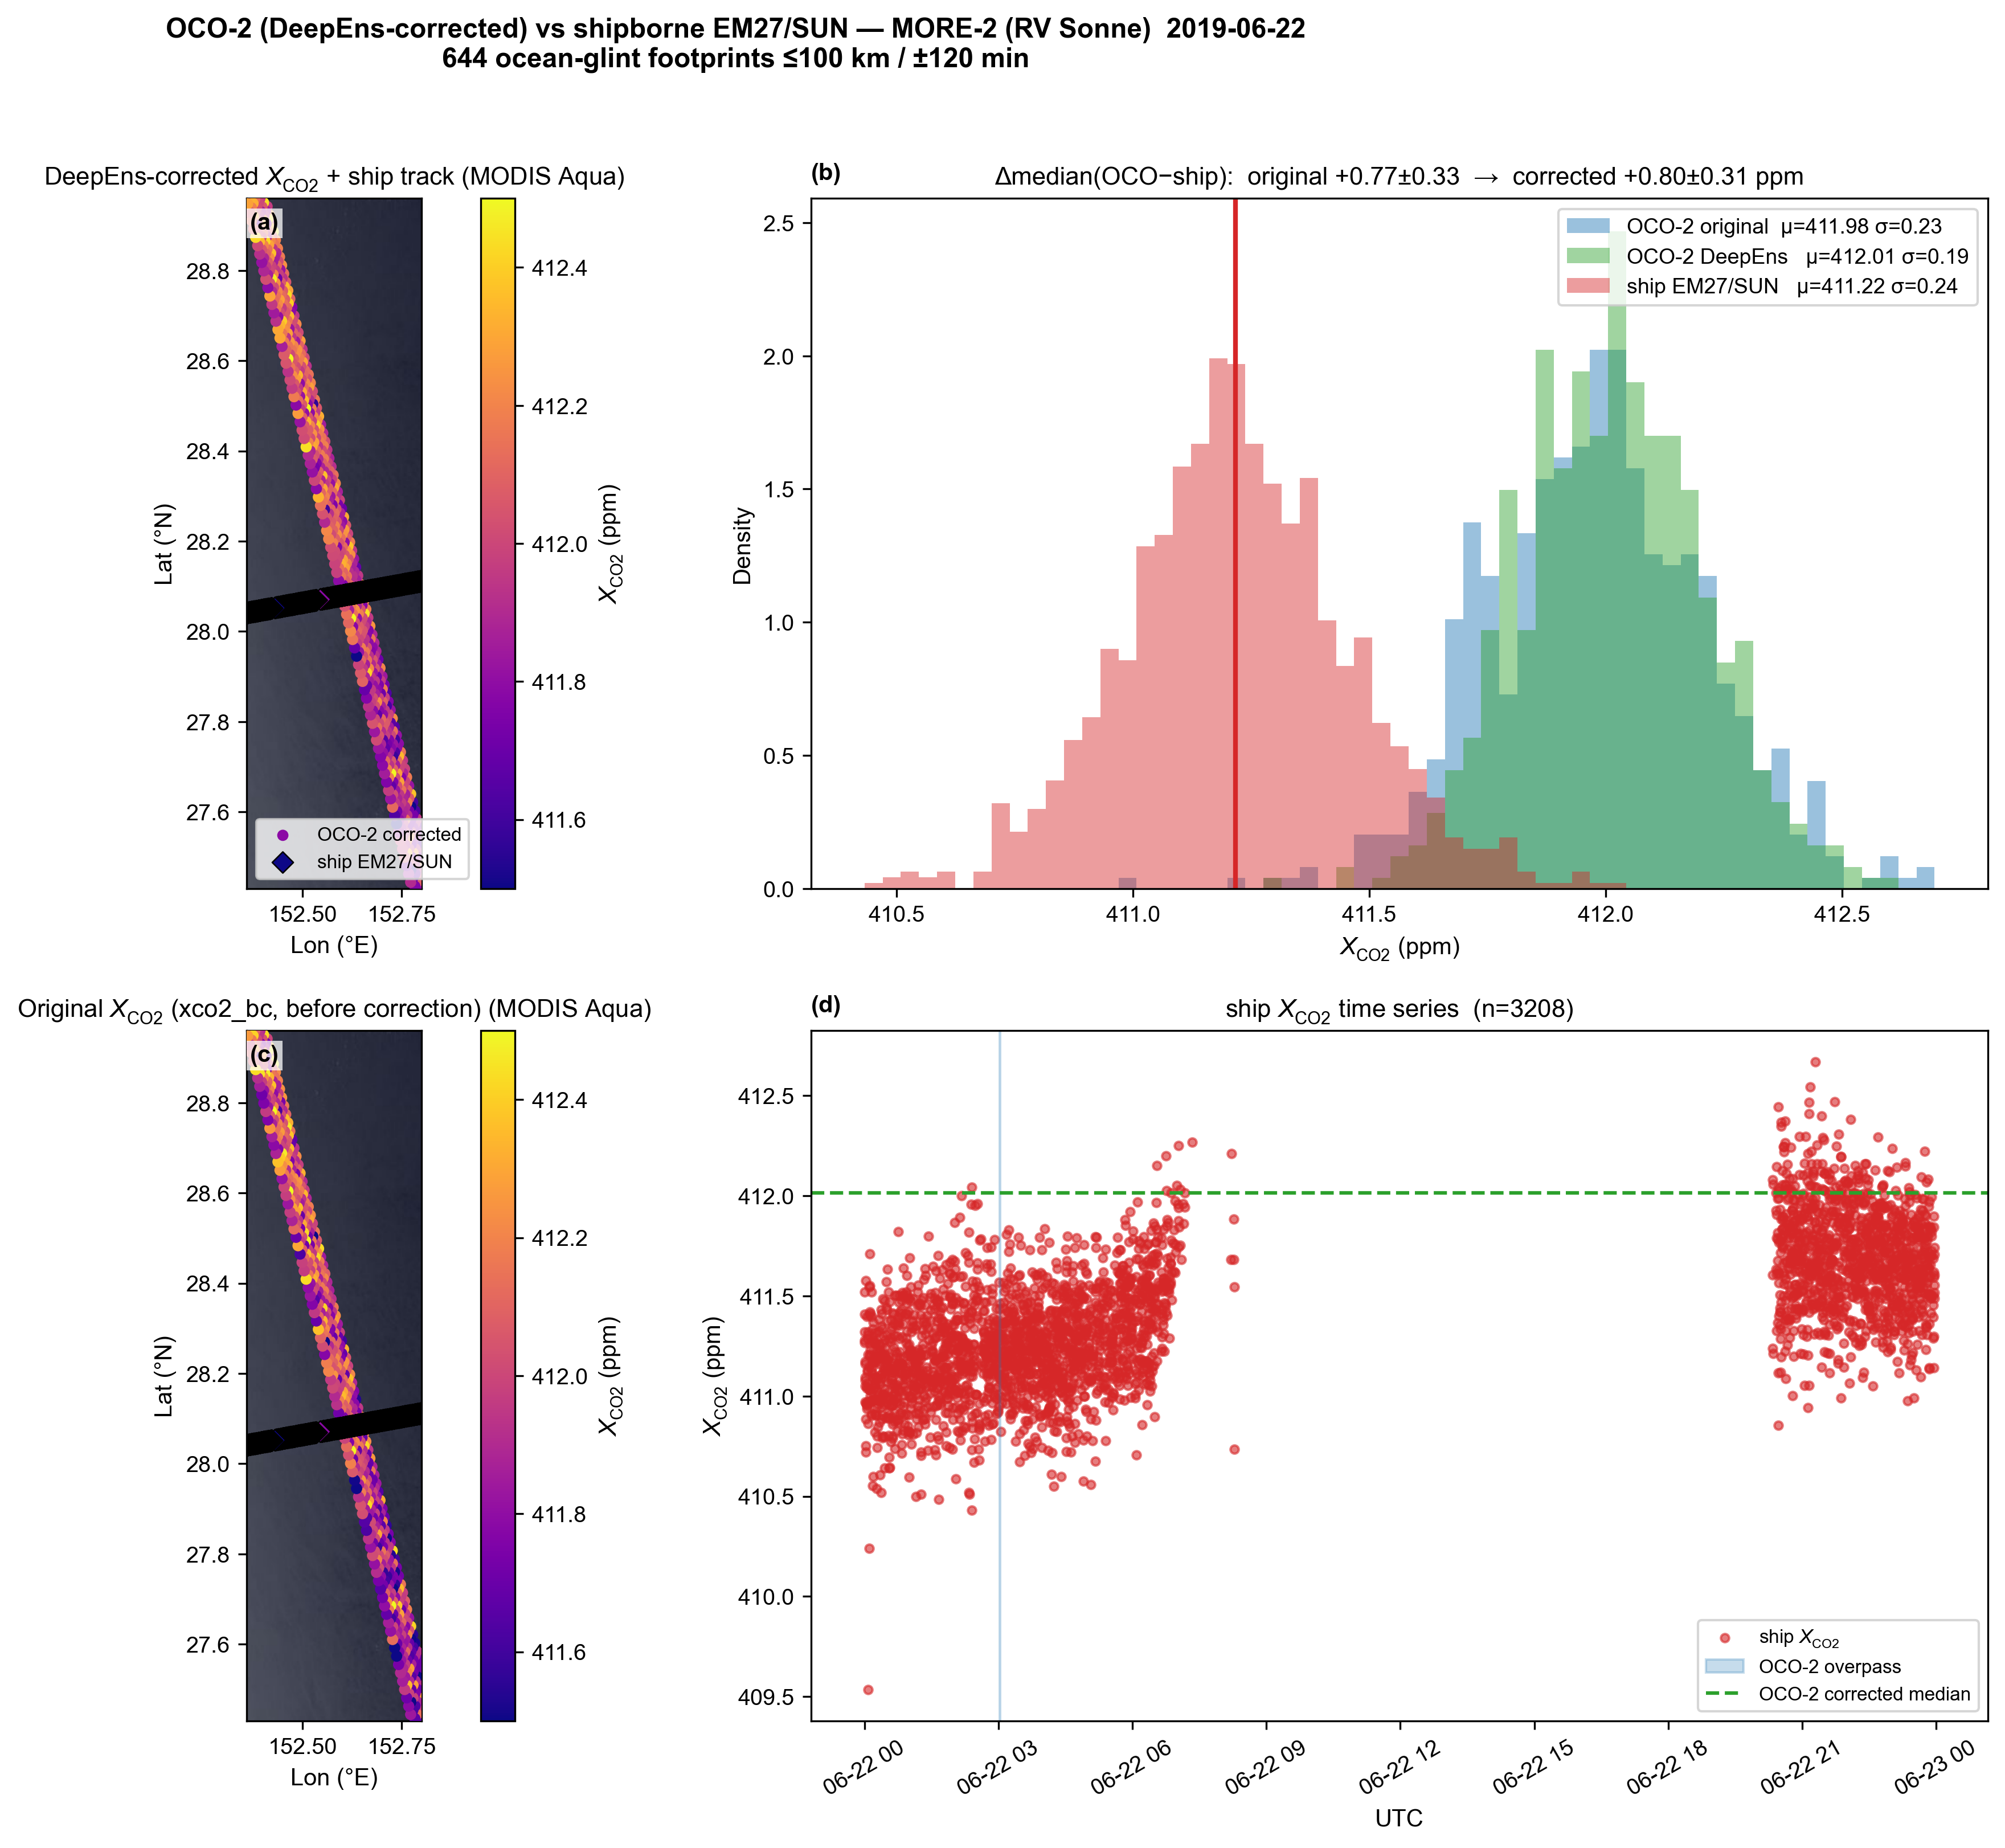
\includegraphics[width=0.8\textwidth]{figures/figE3_ship_clearday_control.png}
\caption{Shipborne clear-day negative control, 22 June 2019 (R/V Sonne EM27/SUN; 1 of 460 footprints within 10 km of cloud): same construction as Fig. E2 against the shipborne column, with the \xcoship time series around the overpass.}
\label{app-fig:ship_far_cld}
\end{figure}





\subsection{Failure cases analysis}
\label{app:tccon-failure}


\FloatBarrier


%\noappendix       %% use this to mark the end of the appendix section. Otherwise the figures might be numbered incorrectly (e.g. 10 instead of 1).

%% Regarding figures and tables in appendices, the following two options are possible depending on your general handling of figures and tables in the manuscript environment:

%% Option 1: If you sorted all figures and tables into the sections of the text, please also sort the appendix figures and appendix tables into the respective appendix sections.
%% They will be correctly named automatically.

%% Option 2: If you put all figures after the reference list, please insert appendix tables and figures after the normal tables and figures.
%% To rename them correctly to A1, A2, etc., please add the following commands in front of them:

  %% needs to be added in front of appendix figures

  %% needs to be added in front of appendix tables

%% Please add \clearpage between each table and/or figure. Further guidelines on figures and tables can be found below.





\authorcontribution{TEXT} %% this section is mandatory

\competinginterests{TEXT} %% this section is mandatory even if you declare that no competing interests are present

\disclaimer{TEXT} %% optional section

\begin{acknowledgements}


We acknowledge the use of imagery provided by services from NASA's Global Imagery Browse Services (GIBS), part of NASA's Earth Observing System Data and Information System (EOSDIS).

\end{acknowledgements}




%% REFERENCES

% Loading bibliography database
\bibliographystyle{copernicus}
\bibliography{refs.bib}

%% The reference list is compiled as follows:

%\begin{thebibliography}{}

%\bibitem[AUTHOR(YEAR)]{LABEL1}
%REFERENCE 1

%\bibitem[AUTHOR(YEAR)]{LABEL2}
%REFERENCE 2

%\end{thebibliography}

%% Since the Copernicus LaTeX package includes the BibTeX style file copernicus.bst,
%% authors experienced with BibTeX only have to include the following two lines:
%%
%% \bibliographystyle{copernicus}
%% \bibliography{example.bib}
%%
%% URLs and DOIs can be entered in your BibTeX file as:
%%
%% URL = {http://www.xyz.org/~jones/idx_g.htm}
%% DOI = {10.5194/xyz}


%% LITERATURE CITATIONS
%%
%% command                        & example result
%% \citet{jones90}|               & Jones et al. (1990)
%% \citep{jones90}|               & (Jones et al., 1990)
%% \citep{jones90,jones93}|       & (Jones et al., 1990, 1993)
%% \citep[p.~32]{jones90}|        & (Jones et al., 1990, p.~32)
%% \citep[e.g.,][]{jones90}|      & (e.g., Jones et al., 1990)
%% \citep[e.g.,][p.~32]{jones90}| & (e.g., Jones et al., 1990, p.~32)
%% \citeauthor{jones90}|          & Jones et al.
%% \citeyear{jones90}|            & 1990



%% FIGURES

%% When figures and tables are placed at the end of the MS (article in one-column style), please add \clearpage
%% between bibliography and first table and/or figure as well as between each table and/or figure.

% The figure files should be labelled correctly with Arabic numerals (e.g. fig01.jpg, fig02.png).


%% ONE-COLUMN FIGURES

%%f
%\begin{figure}[t]
%\includegraphics[width=8.3cm]{FILE NAME}
%\caption{TEXT}
%\end{figure}
%
%%% TWO-COLUMN FIGURES
%
%%f
%\begin{figure*}[t]
%\includegraphics[width=12cm]{FILE NAME}
%\caption{TEXT}
%\end{figure*}
%
%
%%% TABLES
%%%
%%% The different columns must be seperated with a & command and should
%%% end with \\ to identify the column brake.
%
%%% ONE-COLUMN TABLE
%
%%t
%\begin{table}[t]
%\caption{TEXT}
%\begin{tabular}{column = lcr}
%\tophline
%
%\middlehline
%
%\bottomhline
%\end{tabular}
%\belowtable{} % Table Footnotes
%\end{table}
%
%%% TWO-COLUMN TABLE
%
%%t
%\begin{table*}[t]
%\caption{TEXT}
%\begin{tabular}{column = lcr}
%\tophline
%
%\middlehline
%
%\bottomhline
%\end{tabular}
%\belowtable{} % Table Footnotes
%\end{table*}
%
%%% LANDSCAPE TABLE
%
%%t
%\begin{sidewaystable*}[t]
%\caption{TEXT}
%\begin{tabular}{column = lcr}
%\tophline
%
%\middlehline
%
%\bottomhline
%\end{tabular}
%\belowtable{} % Table Footnotes
%\end{sidewaystable*}
%
%
%%% MATHEMATICAL EXPRESSIONS
%
%%% All papers typeset by Copernicus Publications follow the math typesetting regulations
%%% given by the IUPAC Green Book (IUPAC: Quantities, Units and Symbols in Physical Chemistry,
%%% 2nd Edn., Blackwell Science, available at: http://old.iupac.org/publications/books/gbook/green_book_2ed.pdf, 1993).
%%%
%%% Physical quantities/variables are typeset in italic font (t for time, T for Temperature)
%%% Indices which are not defined are typeset in italic font (x, y, z, a, b, c)
%%% Items/objects which are defined are typeset in roman font (Car A, Car B)
%%% Descriptions/specifications which are defined by itself are typeset in roman font (abs, rel, ref, tot, net, ice)
%%% Abbreviations from 2 letters are typeset in roman font (RH, LAI)
%%% Vectors are identified in bold italic font using \vec{x}
%%% Matrices are identified in bold roman font
%%% Multiplication signs are typeset using the LaTeX commands \times (for vector products, grids, and exponential notations) or \cdot
%%% The character * should not be applied as mutliplication sign
%
%
%%% EQUATIONS
%
%%% Single-row equation
%
%\begin{equation}
%
%\end{equation}
%
%%% Multiline equation
%
%\begin{align}
%& 3 + 5 = 8\\
%& 3 + 5 = 8\\
%& 3 + 5 = 8
%\end{align}
%
%
%%% MATRICES
%
%\begin{matrix}
%x & y & z\\
%x & y & z\\
%x & y & z\\
%\end{matrix}
%
%
%%% ALGORITHM
%
%\begin{algorithm}
%\caption{...}
%\label{a1}
%\begin{algorithmic}
%...
%\end{algorithmic}
%\end{algorithm}
%
%
%%% CHEMICAL FORMULAS AND REACTIONS
%
%%% For formulas embedded in the text, please use \chem{}
%
%%% The reaction environment creates labels including the letter R, i.e. (R1), (R2), etc.
%
%\begin{reaction}
%%% \rightarrow should be used for normal (one-way) chemical reactions
%%% \rightleftharpoons should be used for equilibria
%%% \leftrightarrow should be used for resonance structures
%\end{reaction}
%
%
%%% PHYSICAL UNITS
%%%
%%% Please use \unit{} and apply the exponential notation (e.g. 20\,\unit{W\,m^{-2}})


\end{document}
